
\documentclass[refcompress,eversion,noinfo]{XDUthesis}
\usepackage{times}
\usepackage{multirow}
\usepackage{graphicx}
\usepackage{amsmath}
\usepackage{diagbox}
\usepackage{xeCJK}
\usepackage{slashbox}

%自加包

\usepackage{float} %图浮动
\usepackage{algorithm}
\usepackage{algorithmic}


\newcommand{\SWITCH}[1]{\STATE \textbf{switch} (#1)}
\newcommand{\ENDPWITCH}{\STATE \textbf{end switch}}
\newcommand{\CASE}[1]{\STATE \textbf{case} #1\textbf{:} \begin{ALC@g}}
\newcommand{\ENDCASE}{\end{ALC@g}}
\newcommand{\CASELINE}[1]{\STATE \textbf{case} #1\textbf{:} }
\newcommand{\DEFAULT}{\STATE \textbf{default:} \begin{ALC@g}}
\newcommand{\ENDDEFAULT}{\end{ALC@g}}
\newcommand{\DEFAULTLINE}[1]{\STATE \textbf{default:} }
\newtheorem{mydef}{Definition}
\newtheorem{mylm}{Proposition}

\renewcommand{\algorithmicrequire}{\textbf{输入:}}
\renewcommand{\algorithmicensure}{\textbf{输出:}}

% 表格标题与表格内容相距10pt
\newcommand{\topcaption}{
\setlength{\abovecaptionskip}{0pt}
\setlength{\belowcaptionskip}{10pt}
\caption}                       


\newenvironment{varalgorithm}[1]
  {\algorithm\renewcommand{\thealgorithm}{#1}}
  {\endalgorithm}


\graphicspath{{figures/}}

\begin{document}

\XDUfrontmatter

\begin{abstract}
ժҪ��ѧλ���ĵ����ݲ���ע�ͺ����۵ļ�̳�����������Ҫ����ѧλ���ĵ��о�Ŀ�ġ����ݡ��������ɹ��ͽ��ۣ��ص�ͻ��ѧλ���ĵĴ����Գɹ��͹۵㡣ժҪ��������ժҪ��Ӣ��ժҪ��˶ʿѧλ��������ժҪ����һ��Ϊ~1000~�����ң���ʿѧλ��������ժҪ����һ��Ϊ~1500~�����ҡ�Ӣ��ժҪ����������ժҪ���ݱ���һ�£��������������׼��ժҪ�������·���ע�����ĵĹؼ��ʣ��ؼ���һ��Ϊ~3~��~8~�����ؼ��ʺ͹ؼ���֮���ö��Ų���һ��\par
����ժҪ��ʽҪ��Ϊ������С�ġ����˶��롢��������~2~�ַ����о�Ϊ�̶�ֵ~20~����������Ϊ��ǰ~0~�����κ�~0~����\par
Ӣ��ժҪ��ʽҪ��Ϊ��Times New Roman��С�ġ����˶��롢���в��������о�Ϊ�̶�ֵ~20~����������Ϊ��ǰ~0~�����κ�~0~���������֮���һ�С�\par

\keywords{XXX,\quad{}XXX,\quad{}XXX,\quad{}XXX,\quad{}XXX} \par
\end{abstract}

\begin{englishabstract}
The Abstract is a brief description of a thesis or dissertation without notes or comments. It represents concisely the research purpose, content, method, result and conclusion of the thesis or dissertation with emphasis on its innovative findings and perspectives. The Abstract Part consists of both the Chinese abstract and the English abstract. The Chinese abstract should have the length of approximately 1000 Chinese characters for a master thesis and 1500 for a Ph.D. dissertation. The English abstract should be consistent with the Chinese one in content. The keywords of a thesis or dissertation should be listed below the main body of the abstract, separated by commas and a space. The number of the keywords is typically 3 to 5.
\par~\par
The format of the Chinese Abstract is what follows: Song Ti, Small 4, justified, 2 characters indented in the first line, line spacing at a fixed value of 20 pounds, and paragraph spacing section at 0 pound.
\par~\par
The format of the English Abstract is what follows: Times New Roman, Small 4, justified, not indented in the first line, line spacing at a fixed value of 20 pounds, and paragraph spacing section at 0 pound with a blank line between paragraphs.
~\par
\englishkeywords{XXX,\space{}XXX,\space{}XXX,\space{}XXX,\space{}XXX} \par

\end{englishabstract}

\XDUpremainmatter

\begin{symbollist}
\item ~���� \hspace{12em} ��������
\item XXX \hspace{12.5em} XXX
\item XXX \hspace{12.5em} XXX
\item XXX \hspace{12.5em} XXX
\item \ldots
\end{symbollist}

\begin{abbreviationlist}
\item ������\hspace{6em}Ӣ��ȫ��\hspace{6em}���Ķ���
\item ~XXX \hspace{7em} XXX \hspace{7.5em} XXX
\item ~XXX \hspace{7em} XXX \hspace{7.5em} XXX
\item ~XXX \hspace{7em} XXX \hspace{7.5em} XXX
\item \ldots
\end{abbreviationlist}

\XDUmainmatter
\chapter{绪论}

序列(字符串)是现实世界中最基本的信息载体。几乎所有领域的数据信息都可以
抽象成序列来表示,例如普通文本、代码、生物序列、比特流等等。 由于其重要
性,序列(字符串)是所有编程语言中最为基本而重要的数据类型之一。借助于计
算机和序列算法,便可以对不同领域的信息加以处理。因此,研究序列相关的理
论和算法对各个领域来说,都具有基本的重要性。本论文选取了序列挖掘领域三
个重要问题,即模式匹配问题、后缀排序问题、和最长公共子序列问题,进行了
较为深入的研究。下面将分别对这三类问题进行简要介绍。

\section{模式(字符串)匹配}

模式匹配(Pattern Matching, 简称PM), 一直以来都是计算机科学的核心问题之
一。 这里的“模式”特指字符串。 对于很多应用, 例如模式识
别 \cite{Yan2016}, \cite{Xiao2016}, 本体匹配 \cite{Xue2015}
\cite{Xue2016}, 文本分类 \cite{Tang2015} \cite{Zhang2016}, 系统安
全 \cite{Dien2014,Malhotra2016,Fan2016},入侵检测系
统 \cite{Kim2015,Arney2016,Sadotra2016,Lee2017} 等等, 模式匹配算法都是
最为基本而重要的操作。根据待匹配模式的数量,模式匹配技术可以分为两类:
单模式匹配(SPM)和多模式匹配(MPM)。

\begin{figure}[H]
  \centering
  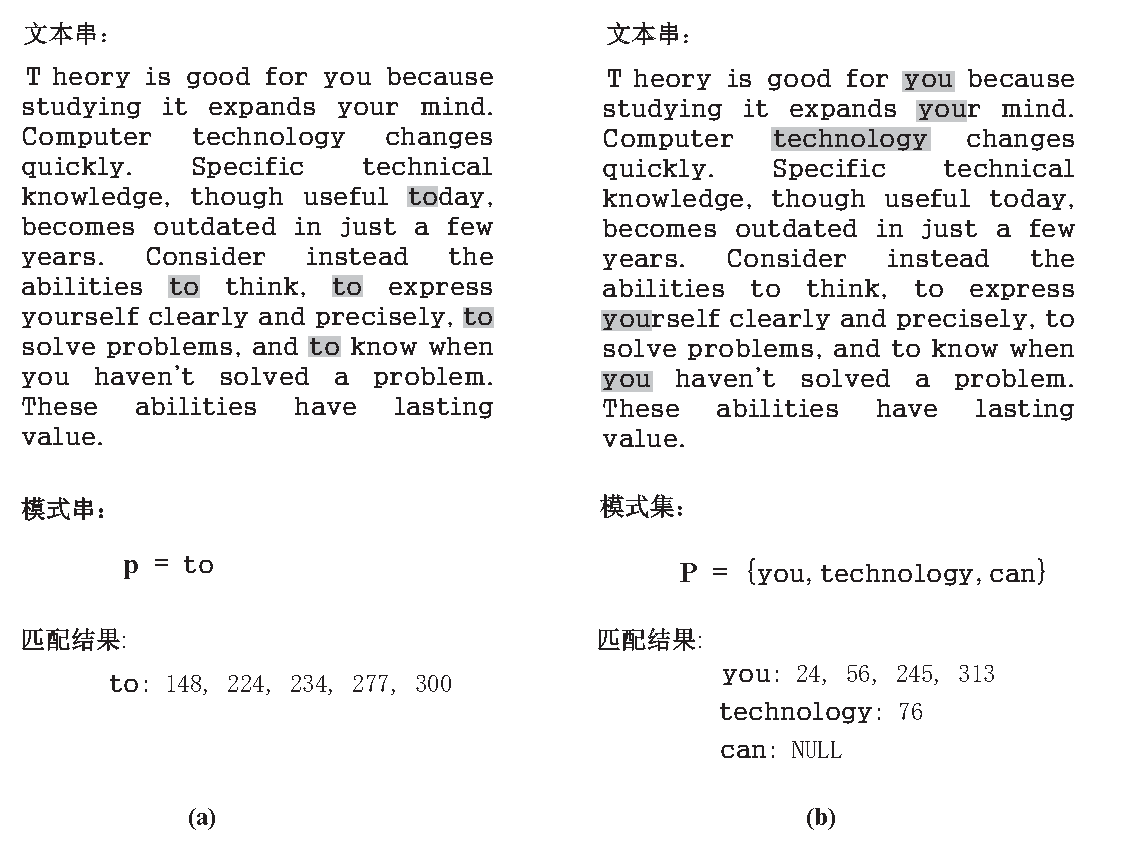
\includegraphics[height=9cm ,width=14cm]{figures/1_Introduction/SPM_MPM.eps}
  \caption{(A) 单模式匹配示例。(B) 多模式匹配示例。}
  \label{fig:SPM_MPM}
\end{figure}


\subsection{单模式匹配}

单模式匹配算法要求在文本串中寻找给定模式串的所有出现位置。如
图 \ref{fig:SPM_MPM} (A) 所示, 给定文本串与模式$to$, 经过匹配发现,模
式串$to$ 出现于文本串中的位置为: 148, 224, 234, 277, 300。

最简单的单模式匹配算法,需要对文本串中的每一个位置与模式串进行逐字符的
比较,一旦出现字符失配,将直接移动到文本串的下一个位置进行匹配。很明显,
当文本串的长度为$n$且模式串的长度为$m$时,这种简单的模式匹配算法的时间
复杂度为$O(m \cdot
n)$。当文本串形如$aaa \dots
a$及模式串为$aaab$时,将出现最坏情况。为此,有更加高效的单模式匹配算法
被提出,最著名的包括KMP \cite{Knuth1977}算法 和 BM \cite{Boyer1977} 算
法。下面将简单介绍这两种算法的主要思想。

1. \textbf{KMP(Knuth-Morris-Pratt)算法}

\begin{figure}[H]
  \centering
  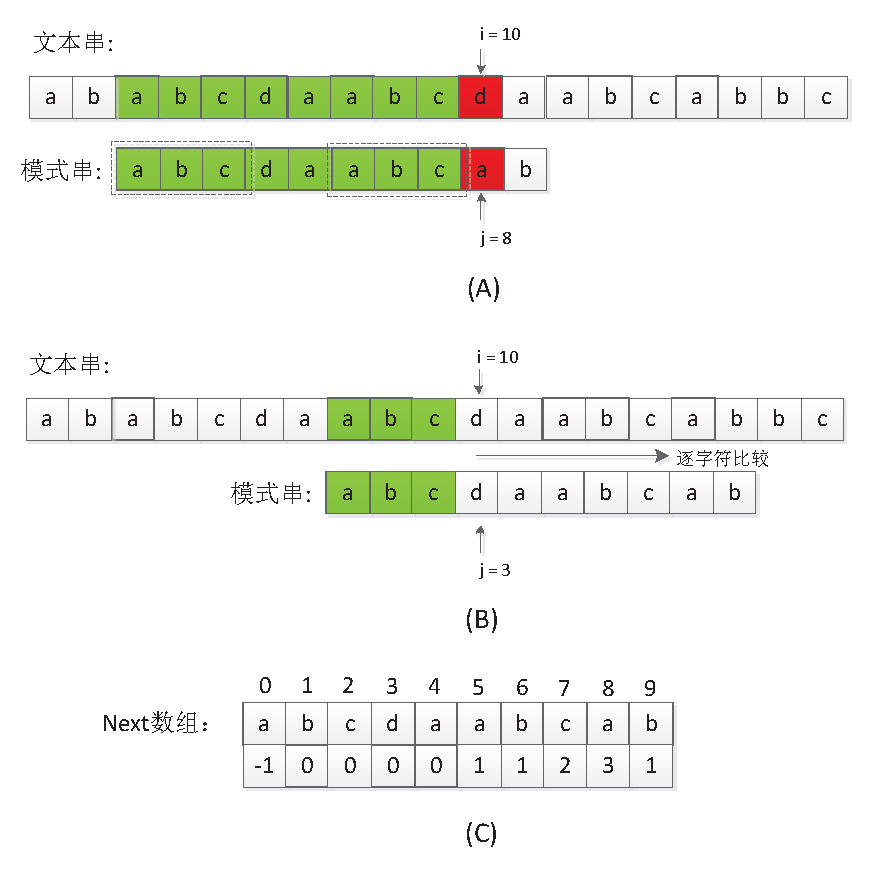
\includegraphics[height=10cm ,width=12cm]{figures/1_Introduction/KMP.eps}
  \caption{KMP算法示例。(A) 第一轮匹配。(B) 第二轮匹配。(C) 模式串
    的Next数组。}
  \label{fig:KMP}
\end{figure}

KMP算法的核心思想在于,一旦匹配失败,可以充分利用已经匹成功的子串信息,
让模式串向右移动尽可能多的位置。右移的位置是这样计算的:在已经匹配的模
式串子串中,找出最长的相同的前缀和后缀,然后向右移动使它们重叠。如
图\ref{fig:KMP}(A)所示,在当前匹配中,文本串中的位置10($i=10$)和模式串
中的位置8($j=8$)出现失配,根据已经匹配成功的子串即$abcdaabc$的信息:该
子串相等的最长前缀与最长后缀是$abc$, 将模式串向右移动使得这两部分相重合,
如图 \ref{fig:KMP}
(B)所示。此时,文本串中当前待匹配位置$i$不变,而模式串中当前待匹配位
置$j$变为3,分别从位置$i$和$j$开始对文本串和模式串进行逐字符比较。KMP算
法在匹配过程中,文本串中的当前匹配位置$i$永不减小,只是当匹配失败时,根
据模式串中的失配位置,来调整模式串中的下一次与文本串位置$i$相比较的位置。
因此,需要知道在失配时,下一次应当用模式串的哪个位置与文本串进行比较。
为此对模式串进行预处理,为其建立失配数组$Next$(如图 \ref{fig:KMP} (C)所
示),如果当前在模式串的位置$j$失配时,下一次将用模式串的位置$Next[j]$来
与文本串进行比较,预处理过程的时间复杂度为$O(m)$($m$为模式串长度)。 由
于匹配过程中, 文本串中的位置$i$永不回溯,所以KMP算法的时间复杂度
为$O(m+n)$ ($n$为文本串长度)。

2. \textbf{BM(Boyer-Moore)算法}

\begin{figure}[H]
  \centering
  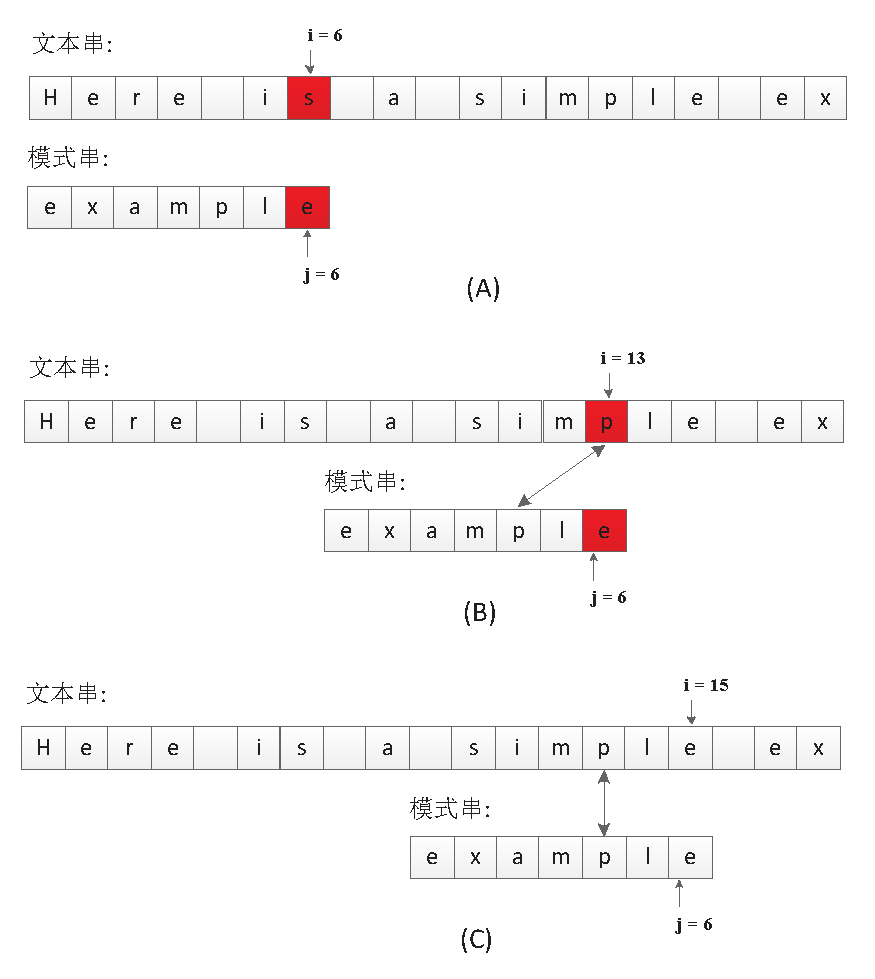
\includegraphics[height=10cm ,width=12cm]{figures/1_Introduction/BM.eps}
  \caption{BM算法示例。(A) 第一轮匹配。(B) 第二轮匹配。(C) 第三轮匹配。}
  \label{fig:BM}
\end{figure}

尽管KMP算法具有线性的时间复杂度,可其实际的速度却并不快。在实际应用当中
(比如各类字处理软件中的字符串查找功能),最常用的单模式匹配算法是BM算
法 \cite{Boyer1977}, 及其诸多变体。BM算法最高效之处在于通过使用“坏字
符”规则,其可以快速跳过文本串中大量的不可能出现匹配的位置。如
图 \ref{fig:BM} (A) 所示,BM算法采用从右到左的方向对模式串与文本串进行
比较,由于第一次比较即失配且文本串中相应的字符$s$没有出现在模式串中,因
此可以将模式串整体向右移动到$s$的下一个字符处,然后再别从位
置13($i=13$)和位置6($j=6$),从右向左地对文本串和模式串进行比较,如
图 \ref{fig:BM}
(B)所示。由于再次失配,且文本串中的字符$p$出现于模式串中,因此将模式串
向右移动2个位置,使两个串中的$p$字符对齐,如图\ref{fig:BM}(C)所示。由
于BM算法在每次匹配失败时,都将根据文本串中的失配字符来移动模式串,因此
需要对整个字符集进行预处理构建坏字符表(表长为$|\Sigma|$,即字符集大
小),当匹配失败时用文本串中的失配字符作为索引来查找坏字符表,来决定需
要将模式串向后移动多少位。BM算法最坏情况的时间复杂度为$O(n \cdot m)$,
但是在实际中很少出现这样的情况。

\subsection{多模式匹配}

多模式匹配要求找出给定模式集中每一个模式串在文本串中的所有出现位置。如
图 \ref{fig:SPM_MPM} (B)
所示,给定模式集$P=\{can, you, technology\}$及文本串,通过多模式匹配发
现, 模式串$you$出现了4次, 模式串$technology$出现了1次, 模式串$can$在
文本串中没有出现。

目前,多模式匹配算法的主要流程是先对模式集进行预处理,构建合适的数据结
构来存储和组织模式集中的模式串,然后用构建好的数据结构和文本进行比较,
一次性找出所有模式集的出现位置。 比较著名的多模式匹配算法包括 AC
\cite{Aho1975} 和 WM \cite{Wu1994} 算法。

1. \textbf{AC(Aho-Corasick)算法}

AC算法是经典的多模式匹配算法,它是KMP算法在多模式环境下的推广,具有线性
时间复杂度。目前,各种AC算法的变体在实际当中被广泛应用。AC算法通过为模
式集构造一个有限状态自动机(DFA),然后将文本串中的每一个字符输入到自动机
中进行状态转移,来实现多模式匹配。图 \ref{fig:AC} 所示的是为模式
集$P=\{he, his, she, hers\}$ 所构造的AC自动机,图中实线箭头及对应字符表
示,在当前状态遇到该字符时应该跳转到的状态,虚线表示在当前状态无匹配字
符时,应该跳转到的状态,图中绿色的状态,表示匹配成功状态。 匹配时,AC算
法将从状态0开始,连续不断地读入文本串中的字符,并根据所读入的字符进行状
态跳转,一旦到达匹配成功状态,将输出匹配到的模式串。 举例说明,假设文本
串为$hers$, 初始状态为0, 第一个文本串字符为$h$, 则自动机将跳转到状态1;
下一个输入字符为$e$,
将跳转到状态2,同时成功匹配模式串$he$并将其输出;下一个字符为$r$,将跳
转到状态8;最后一个字符为$s$,跳转到状态9,并输入匹配成功的模式
串$hers$。传统的AC算法对字符集大小非常敏感,对于较大的字符集,算法所构
造的自动机将会消耗大量的空间,且在实际应用中性能较低。


\begin{figure}[H]
  \centering
  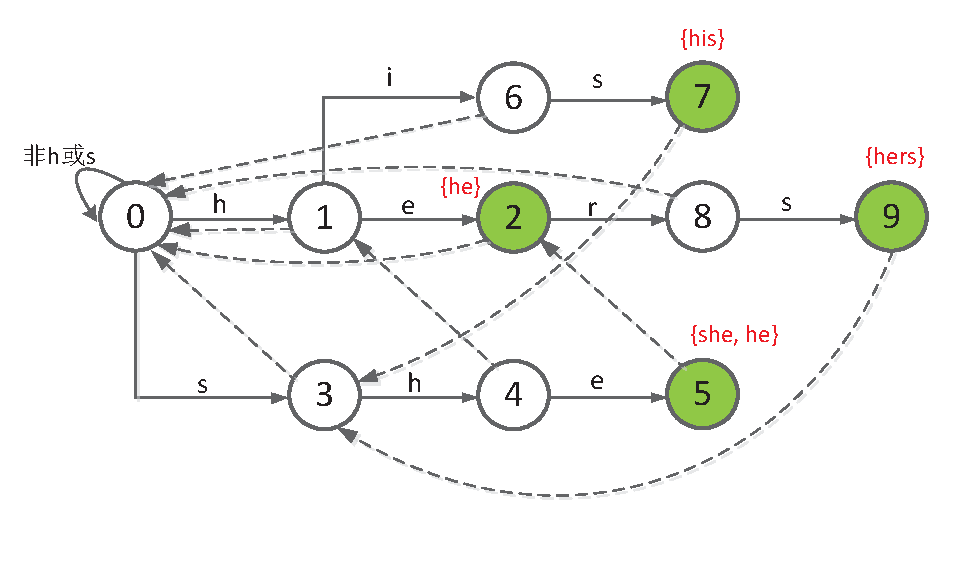
\includegraphics[height=7cm ,width=10cm]{figures/1_Introduction/AC.eps}
  \caption{为模式集$P=\{he, his, she, hers\}$所构建的AC自动机。}
  \label{fig:AC}
\end{figure}

2. \textbf{WM(Wu-Manber)算法}

WM算法是BM算法在多模式环境下的推广,BM算法采用“坏字符”规则在文本中进
行跳跃,而由于模式串个数的增加,WM算法将采用“坏字符块”技术,增大了文
本串和模式串不匹配的可能性.从而增加了直接跳跃的机会。它还使用前缀表进
一步过滤不匹配的模式串,使算法获得了较高的运行效率。

WM算法在预处理时,将为模式集构建3个表结构:哈希表(Hash table),跳转
表(Shift table)和前缀表(Prefix table)。 跳转表用于在扫描文本串的时候,根
据读入字符串决定可以跳过的字符数,如果相应的跳跃值为0,则说明可能产生匹
配,就要使用哈希表和前缀表进一步判断, 以决定有哪些候选模式串, 并通过逐个
比较来找出究竟是哪个或者哪些候选模式串完全匹配。因此,在现有的多模式匹
配算法中,使用块字符跳转、哈希技术和前缀特征表技术的WM算法通常被认为具
有较高的效率,在实际中被广泛使用。 WM算法最优情况下的时间复杂度
为$O(B*n/lsp)$(其中$B$为字符块的长度,$n$为文本串长,$lsp$为最短模式串
长),因此算法性能受最短模式串长的影响较大。 第\ref{chap:WM}章将对WM算
法进行改进。

\section{后缀数组}

后缀数组 (Suffix Array, 简称SA),是由给定字符串的所有后缀按照字典序(由小
到达)排列所构成的数组, 由 Manber和Myers等人提出\cite{Manber1993}, 具有
结构紧凑且空间占用小的优点, 通常作为后缀树 (Suffix Tree) 的空间节省的替
代品, 被广泛地应用于全文索
引 \cite{Strate2015,Fischer2017,Arroyuelo2014},数据压
缩\cite{Louza2015,Chien2015,Pradhan2016,Brisaboa2015} 等领域。

图\ref{fig:suffix}中分别显示了为字符串$bananas$所构建的后缀树以及后缀数
组。由于在给定字符串之后,每个后缀便可由其起始位置完全确定,所以后缀数
组中只需保留后缀的起始位置,相比于后缀树,能够极大的节省存储空间。


\begin{figure}[H]
  \centering
  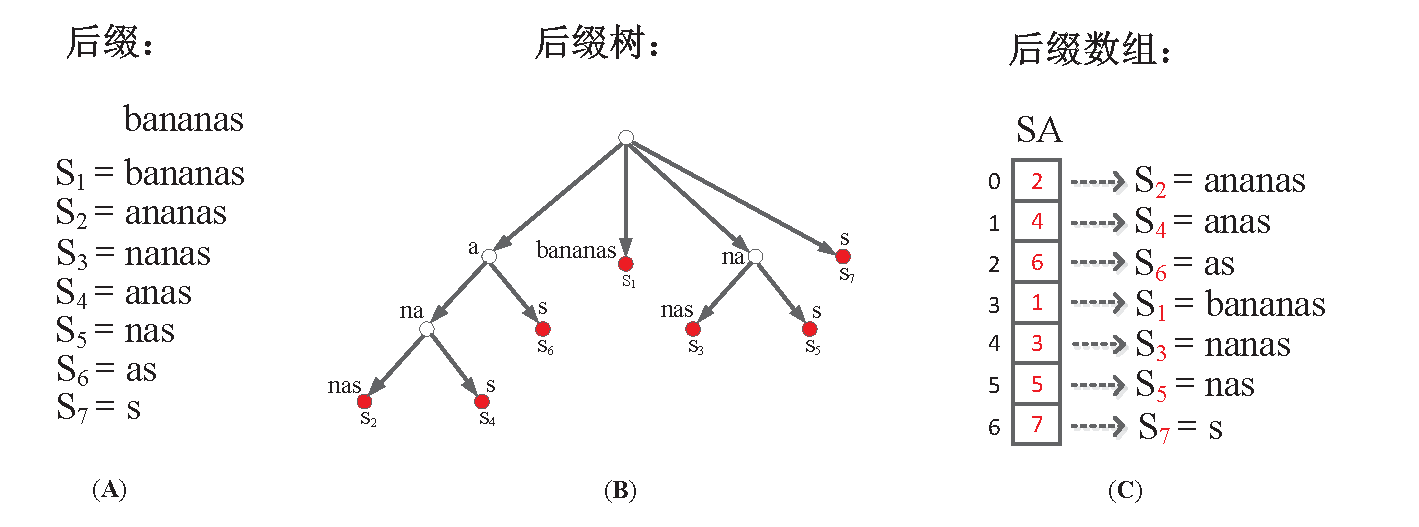
\includegraphics[height=7cm ,width=15cm]{figures/1_Introduction/Suffix.eps}
  \caption{(A) 字符串及其后缀。(B) 对应的后缀树。(C) 对应的后缀数组。}
  \label{fig:suffix}
\end{figure}

通过后缀树能完成的一些文本操作,同样可以通过后缀数组(及一些辅助结构)等
价地完成。例如,上一节中提到的单模式匹配问题,若模式串出现于文本串中,
它必定是某个(些)后缀的前缀,因此可以预先为文本串建立后缀树/数组,然后通
过在后缀树/数组上来查找模式串,可以在极短的时间内完成查找。举例来说,假
设文本串为$bananas$, 模式串为$an$, 对于后缀树,可以从其根节点开始,对模
式串进行逐字符遍历,之后发现有两个后缀即$S_3$与$S_5$都以$an$为前缀,因
此模式串$an$出现于文本串的第3和第5个位置,事实上利用后缀树进行单模式匹
配,可以在$O(m+c)$($m$为模式串长,
$c$为模式串在文本中出现的次数)时间内完成查讯操作。对于后缀数组,可以通
过后缀数组配合最长公共前缀数组,使用基于字典序的二分查找,能够
在$O(m+logn+c)$完成对模式串的搜索。因此,对那些不经常发生变化,且需要频
繁进行查询操作的文本,可以预先为其建立后缀数组(即文本索引),以加快查
询速度。

此外,在很多应用中, 采用后缀数组比采用后缀树可获得更好的时间和空间空性
能。 例如, Pei\cite{Pei2013} 使用后缀树作为基本数据结构, 在字符串上寻找
最短唯一子串, 其时间复杂度为 $O(n^2)$。相比之下, Tsuruta
\cite{Tsuruta2014} 利用后缀数组和最长公共前缀数组作为基本数据结构, 将最
短唯一子串查询的时间复杂度降低到 $O(n)$, 而且空间方面也更节约。

很明显,构建后缀数组的过程本质上就是对后缀排序的过程。对后缀进行排序,
最直接的方法就是先对字符串按照字典序升序构造后缀树,然后对后缀树序深度
优先遍历后缀树,根据遍历到叶子节点的顺序来确定后缀的顺序。由于构造后缀
树能够在线性时间复杂度内完成,因此理论上可以在线性时间内构造后缀数
组。 然而,这种间接地构造后缀数组的方法没有充分利用后缀数组自身的一些的
特性(比如后缀重叠),不仅需要大量的存储空间,而且在实际中极其耗时。为此,
应当研究直接对字符串构建后缀数组的方法,而非间接地通过后缀树来构建。常
见的直接构造后缀数组的方法有前缀倍增算法和DC3算法。

\subsection{前缀倍增}

前缀倍增技术是实际应用当中广泛采用的后缀排序技术。其主要思想是由后缀的
首字符开始,逐步地确定后缀之间的顺序,在第$k$轮中可以根据前$2^k$个字符
来对后缀进行排序,因此对长为$n$的字符串,最多需要$logn$轮即可完成排序。
举例来说,假设需要对字符串$bananas$的后缀进行排序。首先,根据首字符对后
缀进行排序,可将所有后缀分为4组,如图\ref{fig:Prefix_Doubling} (A)所示,
其中,组间有序而组内无序,即前一组中的后缀小于后一组中的后缀,而第1组中
的$S_6$, $S_4$,
$S_2$由于其首字符相同,此时还无法确定顺序,类似地,第3组中
的$S_5$和$S_3$也暂时无法确定顺序。由于$S_6$, $S_4$,
$S_2$首字符相同,因此它们之间的顺序取决于后面的字符串即$s$, $nas$,
$nanas$之间的顺序,这恰好是$S_7$, $S_5$,
$S_3$,由于$S_7$是字典序最大的后缀,所以$S_6$将大于$S_4$与$S_2$,又由
于$S_5$,
$S_3$次序待定,所以$S_4$与$S_2$次序待定。类似地,对于第3组中
的$S_5$和$S_3$,其顺序将由$S_6$与$S_4$决定,由于$S_6$大于$S_4$,$S_5$将
大于$S_3$,如图\ref{fig:Prefix_Doubling}(B)所示。最后,
第1组中$S_4$和$S_2$的顺序将取决于$S_6$和$S_4$, 由于$S_6$大于$S_4$,因
此,$S_4
$大于$S_2$,如图\ref{fig:Prefix_Doubling}(C)所示,排序完成。在本论文
第\ref{chap:SS}章中,将提出一种基于前缀倍增技术的高效的后缀排序算法。

\begin{figure}[H]
  \centering
  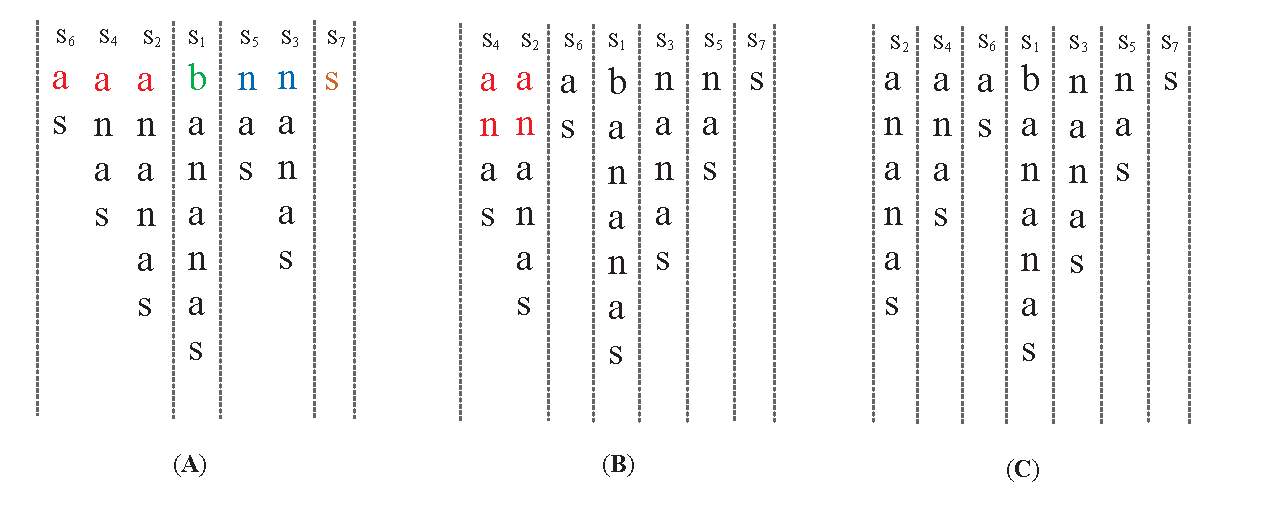
\includegraphics[height=6cm ,width=15cm]{figures/1_Introduction/Prefix_Doubling.eps}
  \caption{利用前缀倍增技术对字符串$bananas$的后缀进行排序。(A) 第一
    轮。(B) 第二轮。(C) 第三轮。}
  \label{fig:Prefix_Doubling}
\end{figure}

\subsection{DC3算法}
\label{sec:KA}

DC3 算法采用分治思想,与 Farach\cite{Farach1997}等人的线性时间后缀树构造
算法过程非常类似,其主要步骤为:

\begin{enumerate}
\item 以递归方式排序后缀$S_i$进行排序,这些后缀在字符串中的起始位置 $i$
  满足: $i~ mod~ 3 \neq 3$。 这使得字符串的规模缩减为原字符串的 2/3。
\item 对第1步所余下的后缀进行排序。
\item 合并步骤 1和步骤 2得到的结果。
\end{enumerate}

DC3 具有线性时间复杂度$O(n)$, $n$为字符串长度。其空间复杂度
为 $O(n/\sqrt{|\Sigma|})$(不包含输入字符串及建好的后缀数组所占空间),这
里$|\Sigma|$为字符集大小,且 $|\Sigma| \in [1, n]$。


\section{最长公共子序列}

度量序列间的相似性是生物信息学及其它领域中的一类基本问题,它们在癌症检
测\cite{Aravanis2017,Chattopadhyay2016,Munday2017},探寻物种的共同起
源 \cite{Zvelebil2007,Perry2015,Donnell2015} 等许多方面具有广泛的应用。
度量序列间相似性最重要手段之一是寻找序列间的最长公共子序列 (Longest
Common Subsequence,简称为LCS), 这已被证实是一类NP难问
题\cite{Maier1978}。根据目标序列的个数,该问题可以被分为两类:(1)寻找两
个序列的最长公共子序列被称为最长公共子序列(LCS)问题;(2) 寻找超过两个序
列的最长公共子序列被称为多最长公共子序列(MLCS)问题。

传统上, 研究工作主要集中于第一类问题。然而近些年来,越来越多的来自生物
信息学及其他领域的应用要求寻找超过两个序列的最长公共子序列(MLCS)。例如,
多序列比对(Multiple Sequence Alignment) 是MLCS问题在生物信息学中最主要
的应用之一 \cite{Katoh2016,Zou2015,Mirarab2015,Bawono2017,Chatzou2015},
该技术能够重排多个DNA,RNA,或蛋白质序列,找出序列间具有相似性的片段,
以此来识别序列间功能性的,结构性的,或进化性的联系。 MLCS算法同样可以应
用到许多其他种类的序列中,比如在自然语言处理中计算字符串之间的编辑距离,
以及应用到许多金融类数据中。

\begin{figure}[H]
  \centering
  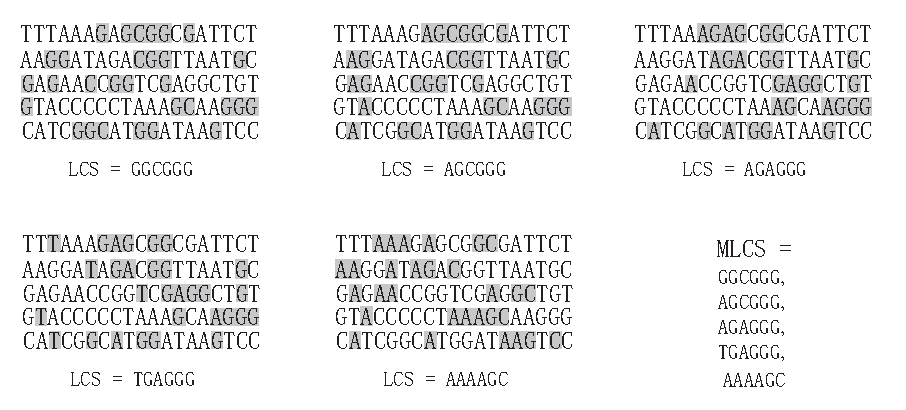
\includegraphics[height=6cm ,width=15cm]{figures/1_Introduction/MLCS.eps}
  \caption{5个DNA序列的最长公共子序列。}
  \label{fig:MLCS}
\end{figure}


图 \ref{fig:MLCS} 显示了给定5个长为19的DNA序列,存在4个长为6的最长公共
子序列。目前,求解MLCS问题通常有两类解决方法:基于动态规划的算法和基于
支配点图模型的算法。

\subsection{基于动态规划的算法}

求解MLCS问题的经典方法基于动态规划 \cite{Smith1981}, \cite{Sankoff1972}。 给定$d$
个序列 $s_1,\, s_2,\,...,\, s_d$, 其长度分别为 $n_1,\, n_2,\, ...,\, n_d$, 基于动
态规划的算法将递归的构造一个具有 $n_1 \times n_2 \times ... \times n_d$ 个元素
的“得分矩阵” $T$, 其中元素 $T[i_1,\, i_2,\, ...,\, i_d]$ 记录了前缀序
列 $s_1[1...i_1]$, $s_2[1...i_2]$, ..., $s_d[1...i_d]$ 的最长公共子序列的长
度。 元素 $T[i_1,\, i_2,\, ...,\, i_d]$ 可由以下公式递归计算:

\begin{equation}
  T[i_1,\, i_2,\, ...,\, i_d] =
  \begin{cases}
    0 & \text{if $\exists j(1 \leq j \leq d), i_j = 0$}\\
    T[i_1-1,\, ...,\, i_d-1] + 1  & \text{if $s_1[i_1] = s_2[i_2] =
      ... = s_d[i_d]$}\\
    max(\bar{T}) & \text{otherwise}
  \end{cases}
\end{equation}

其中$\bar{T} = \{T[i_1-1,\, i_2,\, ...,\, i_d],\, T[i_1,\, i_2-1,\,
...,\, i_d],\, ...,\, T[i_1,\, i_2,\, ...,\, i_d-1]\}$。 一旦得分矩
阵 $T$ 构建完成, 目标序列的最长公共子序列可由 $T$ 的最后一个元
素 $T[n_1,\, n_2,\, ...,\, n_d]$ 向其第一个元素 $T[0,\, 0,\, ...,\,
0]$ 进行反向回溯而得到。 图 \ref{fig:DM} (A) 显示了两个序列 $s_1 =
ACTAGCTA$ 和 $s_2 = TCAGGTAT$ 的得分矩阵 $T$。 如图\ref{fig:DM} (B) 所
示, 这两个序列的最长公共子序 (分别是 $TAGTA$ 和 $CAGTA$), 可由元
素 $T[8,\, 8]$向元素 $T[0,\, 0]$ 进行回溯而得到。

\begin{figure}[!h]
  \centering
  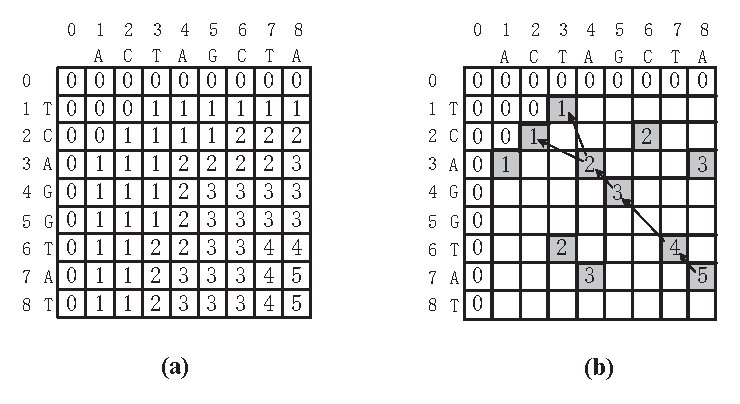
\includegraphics[height=2in, width=4.5in]{figures/1_Introduction/score_table}
  \vspace{1em}
  \caption{(A) 两个DNA序列 ACTAGCTA 和 TCAGGTAT 的得分矩阵。 (B) 通过得分矩阵构建
    最长公共子序列,其中的阴影元素对应于支配点。}
\label{fig:DM}
\end{figure}

很明显,对于具有相同长度 $n$ 的 $d$ 个序列, 使用基于动态规划的算法求解
其MLCS的时间和空间复杂度均为 $O(n^d)$ \cite{Hsu1984}。 已经有许多算法被
提出用于改进基于动态规划方法的效
率 \cite{Hirschberg1977,Apostolico1992,Masek1980,Rick1994}。 然而, 随着
$d$ 和 $n$ 的增加, 所有这些方法的效率仍然无法满足实际需求。

\subsection{基于支配点图的方法}
\label{sec:DP}

目前,主流的MLCS求解方法基于支配点图模型。这些算法首先将对输入序列进行
预处理,为每一个序列构建“后继表”, 然后根据后继表来构造支配点有向无环
图,从而将寻找序列的最长公共子序列问题,转化为寻找有向无环图中从源节点
到终止节点的最长路径问题。然而,现有的基于支配点图的方法会产生大量的节
点,导致内存过量消耗,同时搜索大规模图中的最长路径会相当地耗时。针对此
问题,在本文的第\ref{chap:MLCS}章将提出一种新的图模型来高效的求解MLCS问
题。


\section{本文主要工作及内容安排}
\label{sec:org}

本文针对序列挖掘领域中的三个重要问题:(1) 多模式匹配问题; (2)后缀排序
问题; (3) 最长公共子序列问题进行了研究,分别提出(或改进)了几种高效的
算法。

本文的主要内容安排如下:

第\ref{chap:MPM}章首先介绍了多模式匹配问题的概念及相关工作。然后,针对
现有的基于内存的多模式匹配算法为模式集所构造的数据结构鲁棒性较差,性能
易受到模式集自身特性(尤其是最短模式串长)的影响,同时可伸缩性较差,在处
理大规模模式集时,性能往往无法满足实际需求,提出了一种高效的多模式匹配
引擎。 接着,介绍了该引擎所包括的两个模块:过滤模块基于位图结构,所有操
作均基于底层位运算,因此能够快速地过滤掉文本串中不可能出现匹配的位置;
对每一个潜在的匹配位置,调用核实模块来确认是否有模式串出现。 核实模块基
于一种被称为“自适应匹配树”的树形结构,树中的每个节点都保存了模式集的
一部分片段,节点内部的存储结构将根据自身所保存的模式集片段的特征(即片段
长度和片段数量)进行自适应地调整,以达到时间效率和空间效率的最佳平
衡。 由于每个节点的自适应性,使得对于任何特性的模式集,所构造的自适应匹
配树都能够保持最高效的形态。然后,进一步给出了三种优化的技术:分解自适
应匹配树,节点合并以及节点分裂。将大的自适应匹配树分解成多个小的树结构,
可以提高匹配时的命中率,同时节约内存。节点合并可以将多个单支节点合并为
一个节点,提高算法的运行效率,同时节省内存开销。节点分裂能够减少不必要
的比较操作,进一步提高匹配速度。最后,从鲁棒性和可伸缩性两方面将所提方
法和现有方法进行了对比实验,证明了其具有较好的鲁棒性和伸缩性, 尤其对于
大规模模式集。

第\ref{chap:SS}章首先介绍了后缀排序问题及其相关研究工作。然后介绍了广泛
使用的前缀倍增排序算法---qsufsort算法。针对传统的qsufsort算法存在的缺陷:
在每一轮排序中,所有后缀都将依据定长前缀(即在第$k$轮中,根据每个后缀长
为$2^k$的后缀)被排序,这意味着前$2^k$个字符都相同的后缀,无法在第$k$轮
中被确定顺序,这样,对于那些具有很长公共前缀的后缀,需要许多轮才能被确
定顺序。提出了一种改进型的后缀排序算法---dsufsort,dsufsort算法将记录并
维护后缀数组中每个未排序桶的深度,在每一轮排序中,将根据待排序桶的深度
对其中的后缀进行排序,这使得在第$k$轮中,后缀可以基于长度超过$2^k$的前缀
被排序,从而那些前$2^k$个字符相同的后缀便可在第$k$轮中被确定顺序, 因
此,dsufsort算法仅需要较少的轮数就可以完成排序。 此外,由于桶的深度具有
累加性,因此,对于具有很长公共前缀的后缀,dsufsort算法可以更快速地完成
排序。接着给出了dsufsort算法一些高效的实现技巧,包括:提前对输入字符串
进行变换、在第一轮中采用桶排序对后缀进行排序、以及选择合适的排序函数。
最后,通过实验与现有的算法进行了比较,试验结果证实,对于绝大多数情
况,dsufsort算法的性能要优于对比算法。

第\ref{chap:MLCS}章首先介绍了最长公共子序列问题及其研究现状。然后介绍了
现有的基于支配点图模型的方法。 针对现有的基于支配点图的方法,在构建图时
会产生大量的节点,导致内存过度消耗,同时,在大规模图中搜索最长路径,以
构建最长公共子序列会花费较长的运行时间的问题,提出了一种新的层次化图模
型---Leveled-DAG,及其相应的构建算法。 不同于现有的算法在构造有向无环图
时,需要保存所有产生的节点,并在图构造好之后通过搜索其中的最长路径来构
建相应的最长公共子序列, Leveled-DAG模型可以在建图的过程中实时地构建目
标序列的最长公共子序列,并及时删除那些对构建最长公共子序列没有任何影响
的无用节点。在任一时刻,Leveled-DAG只需保存最新产生的一层节点以及前面产
生的入度不为0的节点,并且,随着构建过程的进行,图中的节点数将会逐渐减少,
最终将仅剩余一个节点,所有目标序列的最长公共子序列都保存在该节点中。 最
后,将所提出的图模型与现有的方法进行了对比实验, 得益于实时地构造最长公
共子序列及删除无用节点,所提模型相比对比算法在时间和空间效率上都有较大
提升。

第\ref{chap:WM}章对WM多模式匹配算法进行改进。首先介绍了WM算法的基本思想
与算法流程,然后对其进行了两方面的改进:(1) 通过寻找每个模式串中出现频
率最少的字符块来确定该模式的特征串,以这样的特征串来构造Hash表避免了出
现过长哈希链的情况,并可将频繁遍历的哈希链中的模式串转移到其它哈希链中,
减少了程序运行中精确匹配的次数,该方法对于包含较短模式的模式集以及模式
集和文本相互有关联的情况,效果尤为明显;(2) 通过为较长的哈希链建立一个
索引表,并通过在该索引表上的二分查找,算法可以在极短的时间内找到需要精
确匹配的模式串,避免了对整条哈希链的遍历,随着模式集规模的增加该方法效
果愈加明显。最后,通过实验证实了改进算法相比原始WM在性能上有较大提升。

第\ref{chap:Conclusion}章对全文进行了总结与展望。





% \begin{abstract}
%   Multi-string matching is a core technique searching a text string
%   for all occurrences of some string patterns. It is widely used in
%   many applications. However, as the number of string patterns
%   increases, most of the existing algorithms suffer from two issues:
%   the long matching time, and the high memory consumption. To address
%   these issues, in this paper, a fast matching engine is proposed for
%   large-scale string matching problems. Our engine includes a filter
%   module and a verification module. The filter module is based on
%   several bitmaps which are response for quickly filtering out the
%   invalid positions in the text, while for each potential matched
%   position, the verification module confirms true pattern
%   occurrence. In particular, we design a compact data structure called
%   Adaptive Matching Tree (AMT) for the verification module, in which
%   each tree node only saves some pattern fragments of the whole
%   pattern set and the inner structure of each tree node is chosen
%   adaptively according to the features of the corresponding pattern
%   fragments. This makes the engine time and space efficient. The
%   experiments indicate that, our matching engine performs better than
%   the compared algorithms, especially for large pattern sets.
% \end{abstract}


\chapter{一种快速的多模式(字符串)匹配引擎}
\label{chap:MPM}

\section{引言}
\label{sec:2_introduction}


多模式匹配(MPM)算法算法需要寻找一个给定模式集中每一个模式串在一个给定文
本串中的所有出现位置。 高效的MPM算法通常只需扫描文本串一次,便可以一次
性找出每一个模式串在文本串中的所有出现。 现有的MPM算法主要包含两个阶段:
即预处理阶段和匹配阶段。 在预处理阶段, 需要为模式集构建一个高效的数据结
构来存储和组织其中的模式串, 然后在匹配阶段,用该数据结构和文本串进行比
较,从而找出每个模式串的出现位置。 显然,预处理阶段为模式集所构造的数据
结构,其时间和空间效率将直接影响算法在匹配阶段的性能。

现今, 在很多应用中,待匹配模式串的数量(即模式集规模) 都非常庞
大。 例如, 现代的杀毒软件和入侵检测系统,其数据库中通常包含了上百万个病
毒特征码或规则序列。 然而, 现有的许多MPM算法无法有效应对于包含大规模模
式集的应用,这主要由两方面原因所致: (1) 这些算法为模式集所构造的数据结
构,其鲁棒性较差,即算法性能受模式集自身特性的影响较大; (2) 所用数据结
构的可伸缩性较差, 这意味着算法在处理大的模式集时效率较低。 例如, 现有很
多算法通常对模式串的长度,尤其是最短模式串的长度,非常敏感, 很多算法无
法有效的处理包含非常短模式的模式集。 因此, 非常有必要设计具有良好可扩展
性和鲁棒性且空间高效的数据结构,用于解决大规模模式匹配问题。

本章, 将提出一种具有良好鲁棒性和伸缩性的匹配引擎,用于处理大规模模式匹
配问题。 类似于现有方法, 所提方法也包含预处理和匹配两个阶段。 在预处理
阶段,将基于模式集来构造匹配引擎;在匹配阶段, 用文本串作为输入数据, 用
匹配引擎进行模式匹配。


所构建的匹配引擎包含“过滤”和“核实”两个模块。 过滤模块能够快速过滤掉
文本串中不可能存在任何匹配的位置(即非匹配位置)。 对于某个存在潜在匹配的
位置, 核实模块将最终确认是否有模式出现于该位置。 引擎所用的过滤模块来
自于 \cite{Lee2013}, 它基于多个位图结构和一组“按位与”及“移位”操
作。 在匹配阶段, 引擎通过查询位图来检查文本串中每个位置是否存在潜在匹
配: 如果当前位置存在潜在匹配, 核实模块将被激活; 否则, 引擎将跳过该位置
并尽可能多地跳过随后的几个位置。 事实上, 过滤模块已经被证实可以充分利用
以前的查询结果,跳过最多的非匹配位置。 基于模式集,我们设计了一种被称
为“自适应匹配树(AMT)”的树形数据结构来作为引擎的核实模块。 具体来说,
整个模式集将被逐步地划分为许多小的片段, 每个片段将被独立地存储于AMT的
节点内,用于后续匹配。 AMT的关键特性是, 每个节点的内部存储结构将会根据
其所存储的模式片段的特性进行自适应选择,即图中每个节点都有自己独立的内
部结构。 这种自适应性使得每个节点在匹配速度和空间效率方面保持了良好的平
衡, 也使得最终的AMT在匹配阶段非常高效。

本章组织如下: \ref{sec:2_RW} 节回顾了MPM领域的相关工
作。  \ref{sec:2_notations}节介绍了用到的一些符号和术
语。 \ref{sec:filter}节 介绍了过滤模块。 \ref{sec:verification}节 介绍
了核实模块。 \ref{sec:2_experiments}节 进行了对比实
验。\ref{sec:2_conclusion} 节对本章进行总结。

\section{相关工作}
\label{sec:2_RW}

由于模式匹配问题的重要性, 在过去几十年里, 学者们提出了很多有效的算
法。 比较知名的算法包括: Knuth-Morris-Pratt (\textsf{KMP})
\cite{Knuth1977}, Boyer-Moore (\textsf{BM}) \cite{Boyer1977},
Wu-Manber (\textsf{WM}) \cite{Wu1994}, and Aho-Corasick (\textsf{AC})
\cite{Aho1975}。 其中 \textsf{KMP} 和 \textsf{BM} 算法只适用于单模式匹配
问题。  \textsf{AC} 算法是KMP算法在多模式下的推广, 通过对模式集构造有
限状态自动机(DFA), 使得所有模式串可以同时被匹配。 它是第一个具有线性时间
复杂度的MPM算法, 然而其实际匹配速度并不很快, 而且, AC算法对字符集大小非
常敏感, 通常需要大量的存储空间来构造DFA, 这限制了它在一些领域的应用。

为了减少\textsf{AC} 算法的存储开销, Tuck \cite{Tuck2004} 提出
了 Bitmapped AC 算法。 在每个状态节点中, 该算法使用位图结构来取代传统的
指向孩子的指针。 另外, 该算法使用了路径压缩技术来合并单支路径上的状
态。 然而, 从一个状态转移到另一个状态需要检查位图中所有的位(共256个)并
将其相加, 这使得该算法的平均性能并不高。 另一个旨在减少AC空间消耗的算法
是由 \cite{Bremler2011} 提出的 \textsf{Compressed AC} 算法。 除了使用类
似的路径压缩技术之外, 该算法还使用了可以消除叶节点状态的技术。 实验结果
显示, 相比传统AC算法, \textsf{Compressed AC} 最多可以减少 $60\%$ 的空间
消耗, 但是仅仅对于某些模式集才具有如此效果。 Lee \cite{Lee2013} 提出了
被称为 \textsf{Pre-filter+AC} 的算法, 该算法包含一个预过滤器和一个检测
引擎。预过滤器用于寻找文本串中, 潜在的匹配位置。 一旦该位置被找到, 检测
引擎将被激活, 用于确认最终的匹配结果。 预过滤器使用一个被称为“主位
图”的比特向量和一些基本的“按位与”及“移位”操作来记录和处理查询结
果。 而检测引擎则是AC自动机的一种变体, 可以一次性检测所有的模式串。 然
而, 如作者所说, 预过滤器仅对较长的或中等长度的模式串有较好的效果, 而对
于短模式串,过滤效果将大打折扣。 近期, Kim \cite{Kim2015} 提出了一种被称
为 \textsf{Split} 的内存高效型算法, 用于深度包检测系统, 该算法由多
个DFA组成, 适合于并行化匹配。

\textsf{WM} 算法是另一个被广泛应用的高效的MPM算法, 在实际应用中, WM通常
快于\emph{AC}。 \textsf{WM} 算法可以被视为是 \emph{BM} 算法在多模式下的
推广。 它使用了和\emph{BM}算法类似的“跳转表”, 但是其跳转不是
像 \emph{BM} 那样基于单个字符, 而是基于包含$B$个字符的字符块 (在实际中,
$B$通常取2或3)。 WM算法的时间复杂度为 $O(B \cdot n/lsp)$, 其中 $n$ 是文
本串的长度, $lsp$ 是最短模式串的长度。 由此可见, 最短模式串的长度会
对 WM 算法的性能造成严重影响。

为了改进 \textsf{WM} 算法, Zhou \cite{Zhou2007} 提出了 \textsf{MDH} 算
法。 不像WM算法那样总是使用每个模式串的前 $m$ 个字符作为其标签,
\textsf{MDH} 采用了启发式策略来选择最优的 $m$ 个连续字符作为模式串的标
签。 类似地, Zhan \cite{Zhan2014} 使用了不同的策略来选择每个模式串的标
签, 另外, 作者还设计了一种索引结构来提高对哈希表中候选模式串的搜索速
度。 这些算法都提高了WM算法在处理普通模式集时的性能, 但是它们并没有解决
由短模式串所造成的算法性能低下。 为了解决该问题, Zhang
\cite{Zhang2009a}提出了\textsf{HCWM}算法, 该算法会将长度小于4的模式串单
独分离出来, 对于这些短模式串, 算法将使用独立的数据结构和不同的匹配策
略。 该方法可以确保被分离出的短模式串和其他模式串同时被匹配。 另一个应对
此问题的方法, 是由 Choi \cite{Choi2011} 提出的 \textsf{$L^{+1}$-MWM} 算
法, 该算法通过对短模式串附加一个虚拟字符, 来降低短模式串的负面影响。 作
者称, 相比WM算法, \textsf{$L^{+1}$-MWM} 算法的性能平均提高
了 $20\%$, 当$lsp < 5$时, \textsf{$L^{+1}$-MWM} 的性能提高
了 $38.87\%$。


在大数据环境下, 大规模模式匹配问题正变得越来越重要。 Le \cite{Le2013}提
出了一种基于流水线二叉树的内存节约型框架构--\textsf{MASM} 用于解决大规
模模式匹配问题, 它使用了被称为“leaf-attaching”的技术来对给定模式集进
行压缩, 被压缩过的模式集将被进而转化为一棵流水线二叉查找树, 用于在匹配
阶段。 Moraru \cite{Moraru2012} 提出了一种内存节约及cache友好型的算法,
用于处理大模式集。 该算法基于 Rabin-Karp \cite{Karp1987} 单模式匹配算法
构造, 包含了一种新的前向反馈布隆过滤器, 该过滤器能够充分利用现代计算机
的内存架构。 该算法同样适宜在GPU上进行并行化实现。

目前, 有许多研究致力于通过硬件来加速现有的MPM算法。 Agarwal
\cite{Agarwal2013} 提出了一种硬件架构用于信息抽取技术, 使其具有较高的吞
吐率。 该架构使用了基于哈希的技术, 而非传统的基于DFA的技术。 基于DFA的方
法 (比如 \textsf{AC}) 在一个时钟周期内通常只能处理一个字符, 而该算法所
用的基于哈希的技术在一个时钟周期内可以处理多个字符, 相比基于DFA的方
法,具有更高的吞吐率。 Zhang \cite{Zhang2015} 提出了基于 GPU 的并行化算
法 \textsf{G-PEBF}, 该算法使用了扩展的布隆过滤器, 将模式集分为 $N$ 个子
集, 每个子集所包含相同长度的模式串。 然后算法为每个子集构造一个扩展的布
隆过滤器, 并在GPU上使用 $N$ 个线程进行并行处理。 \textsf{G-PEFB} 算法的
性能高度依赖于匹配过程中所使用的线程的个数, 同时, 该算法不适于处理包含
较短模式的模式集。 Sidler \cite{Sidler2017} 提出了使用GPU-CPU混合架构的
模式匹配算法。 Nemeth \cite{Nemeth2016} 使用FPGA来对传统的多模式匹配框
架YARA进行加速。Sotiropoulou \cite{Sotiropoulou2017} 对在嵌入式系统中的
实时多模式匹配问题进行了深入的研究。

如今, 已有许多对经典 MPM 问题的扩展被提出。 Tomohiro \cite{I2015} 介绍
了一种 MPM 问题的变体, 其中模式集以一种可以由直接程序(straight line
program)来表示。  Khancome \cite{Khancome2013} 介绍了动态 MPM 问题并提
出了相应的算法。 该算法使用倒排列表数据结构, 使得模式集可以在最短时间内
得到更新。 Amir \cite{Amir2015} 提出了“有间断”的MPM 问题, 其中模式集
中的每个模式串都由一些通配符进行分隔。 Neuburger \cite{Neuburger2012}
提出了一种能够在小空间内, 对二维MPM问题进行处理的算法。

\section{相关概念}
\label{sec:2_notations}

令 $\Sigma$ 表示有限个字符组成的字符集 (本章只关注于ASCII字符
集, 即 $|\Sigma| = 256$ 且每个字符占用一个字节的存储空间。)  给定字符
集 $\Sigma$, $\Sigma$ 上的字符串及其子串定义如下:

\textbf{定义 1.}  $\Sigma$ 上的字符串是由有限个 $\Sigma$ 中的字符组成的
序列。 长为 $n$ 的字符串表示为 $S = c_1c_2..c_n$, 其中 $S$ 的第 $i$个字
符表示为 $S[i] = c_i \in \Sigma$ $(1 \leq i \leq n)$。  $S$ 的长度表示
为 $|S|$。 $S$ 的一个子串是由 $s$ 中任意个连续字符所构成的字符串。  $S$中,
起始于位置 $i$ 且长为 $len$ 的子串可表示为 $S[i,\,len]$。

给定字符串 $S$, 它的前缀和后缀都是 $S$ 特殊的子串, 定义如下:

\textbf{定义2.} 字符串 $S$ 长为 $m$ 的前缀, 是由 $s$ 前 $m$ 个字符构成
的子串, 表示为 $S^{+m}$, 即 $S^{+m}=S[1,\,m]$。  起始于 $S$ 第 $m+1$ 个
位置的后缀, 是由 $s$ 去掉前 $m$ 个字符所留下的子串, 表示
为 $S^{-m}$, 即 $S^{-m} = S[m+1,\,|S|-m]$。 (注意, 字符串 $S$
是它本身的前缀同时也是后缀, 即 $S=S^{+|S|}=S^{-0}$。)

最后, MPM 问题定义如下: 

\textbf{定义 3.} 给定文本串 $T$ 和模式
集 $P=\{p_1,\,p_2,\,\dots,\,p_k\}$, 其中 $T$ 和 $p_i$ $(1 \leq i \leq
k)$ 均是 $\Sigma$ 上的字符串。 多模式匹配问题就是要找出 $P$ 中每一个模
式串在 $T$ 中的每一次出现, 即需要构建结果集合
$R = \{(i,\, p_j)\;|\; p_j \in P\; and\,\; T[i,\,|p_j|]=p_j\}$。


\section{过滤模块}
\label{sec:filter}

如前所述, 匹配引擎包含过滤模块和核实模块。 本节将介绍前者, 下节将介绍后
者。

引擎中所采用的过滤模块来自于 \cite{Lee2013}, 它是WM算法中过滤器的改
进。 类似于WM算法, 给定模式集, 只有每个模式串中长为 $lsp$ 的前缀用来构
造过滤模块, 其中 $lsp$ 是模式集中最短模式串的长度。 同WM算法类似, 过滤
操作是基于字符块的 (字符块是只包含少量字符的字符串) 而非单个字符。 假设
每一个字符块包含 $k$ 个字符, 过滤模块将包含 $lsp-k+1$ 个查询位图, 表示
为 $B_1$, $B_2$, \dots, 和 $B_{lsp-k+1}$, 其中每个位图都是有 $N$ 个比特
的位向量。  (通常, 若 $lsp \leq 5$, 令 $k = 2$; 否则, 令 $k=3$。$N$ 被
设置为 $|\Sigma|^k$)。 令 $B_j[i]$, $0 \leq i \leq N - 1$,
$1 \leq j \leq lsp-k+1$, 为第 $j$ 个查询位图的第 $i$ 个比
特, 且 $B_j[i]$ 被设置为1, 当且仅当存在模式
串 $p_m$ 使得 $hash(p_m[j,k]) = i$ ($p_m[j,k]$ 是一个起始于模式
串 $p_m$ 第 $j$ 个位置的长为 $k$ 的子串), $hash$ 是一个哈希函数, 能够将
长为 $k$ 的字符块映射到范围在 $[0, N-1]$ 内的整数。

\begin{figure}[H]
  \centering
  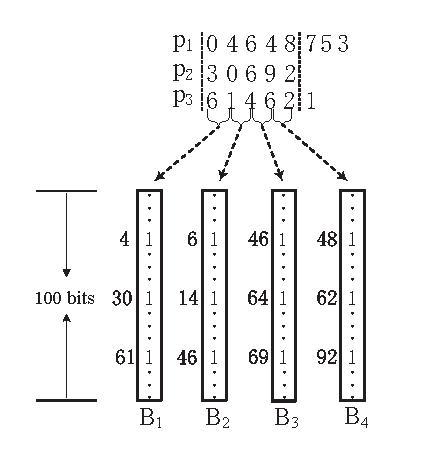
\includegraphics[height=2.5in, width=2.5in]{figures/2_MPM/filter.eps}
  \caption{为3个数字模式串所构造的过滤模块}
  \label{fig:filter}
\end{figure}

图 \ref{fig:filter} 给出了过滤模块的一个例子, 假设字符集为
$\Sigma = \{0, 1, 2, \dots, 9\}$, 且模式集为 $P = \{p_1,\; p_2,\;
p_3\}$, 其中 $p_1 = 04648753$, $p_2 = 30692$, $p_3 = 614621$。 很明显,
$lsp = |p_2|= 5$。 假设 $k = 2$, $N = 100$, 且哈希函数是恒同映射。 对于这
样的情况, 过滤模块将包含 $lsp - k + 1 = 4$ 个查询位图, 即 $B_1$,
$B_2$, $B_3$, $B_4$, 且其中有 $B_1[i] = 1$ 当且仅当 $i$ = 4, 30, or
61; $B_2[i] = 1$ 当且仅当 $i$ = 6, 14, or 46; $B_3[i] = 1$ 当且仅
当 $i$ = 46, 64, or 69; 以及 $B_4[i] = 1$ 当且仅当 $i$ = 48, 62, or
92。

一旦查询位图构造完成, 便可以用来过滤文本串中的位置。 在过滤操作中,一个长
为 $lsp$ 的滑动窗口 $W$ 被用来在文本串 $T$ 中选取子串。 最初,
$W$ 与 $T$ 的最左端对齐, 所以 $W$ 包含的 $T$ 的子串为 $T[1,lsp]$。 一般
地, 假设 $W$ 移动到 $T$ 的第 $i$ 个位置, 且 $W$ 中包含的子串
为 $T[i,lsp]$。 接着 $T[i,lsp]$ 末尾长为 $k$ 的字符块, 即 $T[i+lsp-k,
k]$ 被用作输入来查询所有的位图。 令单个比特位 $qb_j$ 为 $B_j$ 的输
出 ($1 \leq j \leq lsp - k + 1$), 且 $qb_j=1$ 当且仅
当 $B_j[hash(T[i+lsp-k,k])] = 1$。 令结果位图
$QB = qb_1qb_2 \dots qb_{lsp-k+1}$ 表示当前的查询结果, 用主位图
$MB = mb_1mb_2 \dots mb_{lsp-k+1}$ 来累加以前的查询结果, 并作为过滤模块
当前的状态向量。 最初, 主位图 $MB$ 的所有位都被设置为 1。 在得到一个查询
结果 $QB$ 之后, 主位图将被更新为 $MB = MB \; \& \; QB$, 其中 \& 是''按
位与''操作。 对于更新后的 $MB$, 如果 $mb_{lsp-k+1} = 1$, 则位置 $i$ 是一
个潜在匹配点, 且将激活核实模块。 否则, 滑动窗口 $W$ 将前进 $lsp-k+1$ 个
位置, 如果 $MB$ 所有的位都为 0; 或前进 $lsp-k+1-r$ 个位置, 若 $mb_r=1$
且 $mb_i=0$, $r < i \leq lsp-k$。 被滑动窗口 $W$ 跳过的位置都已经被过滤
掉。  如果 $W$ 将前进 $h$ 个位置, 则将 $MB$ 右移 $h$ 位且向左边空出来的
位补1。 值得注意的是, 在 \cite{Lee2013} 中作者已经证实, 过滤模块可以最大
化地利用以前的查询结果, 在滑动窗口每次前进的长度方面是最优的 (即可以过
滤掉尽可能多的位置)。

\begin{figure}[H]
  \centering
  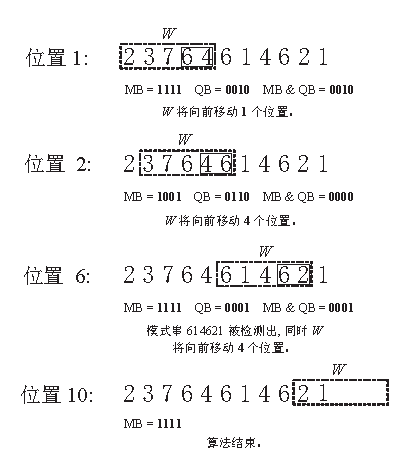
\includegraphics[height=3in, width=3in]{figures/2_MPM/filtering}
  \caption{使用过滤模块过滤文本中的非匹配位置。}
  \label{fig:f_match}
\end{figure}

举例说明, (见图 \ref{fig:f_match}), 考虑前面构造好的查询位图, 同时假
设 $T=23764614621$。  最初, 滑动窗口 $W$ 包含23764 且 $MB = 1111$。
23764末尾的长为2的字符块, 即64, 被用作第一次查询, 且查询结果
为 $QB=0010$。 由于 $MB\; \&\; QB = 0010$, $W$ 将前进一个位置 (即 $T$ 的
第一个位置已被过滤掉), 接着 $MB$ 会右移1位且左边补1, 变成 $1001$。 对于
第二个位置, $W$ 中所包含的子串为37646。 此时, 字符块46被用来查询位图, 查
询结果为 $QB=0110$。 由于 $MB\; \& \; QB=0000$, $W$ 将向前移动4个位置到
位置6 (第 $2 \sim 5$ 位被过滤掉了), 且 $MB$ 将被更新为1111。 对于位置6,
$W$ 包含61462, 字符块62将被用来进行查询得到 $QB = 0001$。 由于 $MB\; \&
\; QB = 0001$, 位置6是一个潜在匹配位置, 此时将激活核实模块。 经过核实,
模式串 $p_3=614621$ 出现于位置6。 接着, $W$ 向后移动4位到达位
置10。 然而, 由于此时 $W$ 中剩余子串的长度小于 $lsp$, 这意味着不可能再有
任何模式串出现, 因此, 整个算法结束。

\section{核实模块}
\label{sec:verification}

核实模块是整个匹配引擎的核心, 其决定了引擎性能的下界 (即最差性能)。 核实
模块基于一种被称为自适应匹配树(AMT)的新型数据结构, 它是经典trie树结构的
一种改进。 类似于trie树, 但是以一种更加高效灵活的方式, AMT能够进行快速的
成员查询, 以此来决定给定字符串是否存在于模式集中。 接下来将介绍AMT的构建
方式, 和进一步的优化技术。

\subsection{构建AMT}
\label{subsec:amt}

AMT基于模式集构建, 总体来说, 构建过程包含以下5个主要步骤:

\begin{enumerate}
\item 创建后缀集 $SF$ 并将模式集中的所有模式串放入 $SF$。 每个模式串都视
  为它自身的一个后缀。
\item 计算 $SF$ 中最短后缀的长度, 用 $lss$表示。 对于 $SF$ 中的每一个后
  缀, 去掉其长为 $lss$ 的前缀, 所有被移除的前缀构成前缀
  集 $PF$。 对 $PF$ 进行去重, 同时计算 $|PF|$, 即不同前缀的数
  量, 用 $ndp$ 表示。
\item 产生一个树节点 $node$ 来保存 $PF$ 中的所有前缀。 $node$ 本质上是一
  个索引结构, 以其所保存的前缀作为键。 节点 $node$ 的内部结构, 会根据上
  一步中计算出的 $ndp$ 和 $lss$ 进行自适应选择。 有多种结构可供选择。
\item 将 $SF$ 中具有相同(但已被移除的)前缀的后缀聚集起来, 形成子后缀
  集。 将每个子后缀集与其在 $node$ 中对应的前缀关联起来。
\item 对于上一步产生的每个子后缀集, 从步骤2开始, 重复执行同样的过程。直
  到不再产生新的子后缀集。
\end{enumerate}

\begin{figure}[H]
  \centering
  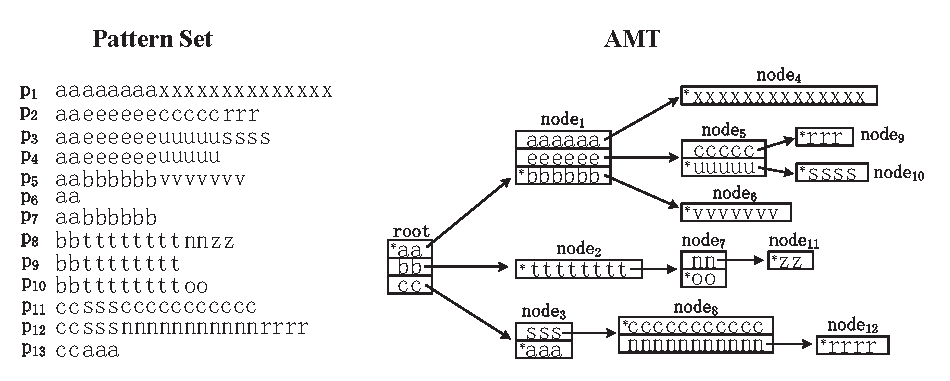
\includegraphics[width=\textwidth]{figures/2_MPM/AMT}
  \caption{从模式集构造AMT。 AMT中的每个箭头代表一个指向孩子节点的指针。}
  \label{fig:AMT}
\end{figure}

作为一个例子, 图 \ref{fig:AMT} 显示了从模式集
$P = \{p_1,\, p_2,\, \dots,\, p_{13}\}$ 构造AMT的过程。 注意, 由于每个
模式串都是自身的一个后缀, 模式集 $P$ 也可以被看作一个后缀集 $SF$。 首先,由
于 $p_6$ 是 $P$ 中最短的模式串(后缀), 所以 $lss = |p_6| = 2$。 接着,
移除掉每个模式串(后缀)长为2的前缀, 所有被移除掉的前缀构成了前缀集:
$PF = \{p_1^{+2} = aa,\; p_2^{+2} = aa,\; \dots,\; p_{13}^{+2} =
cc\}$。  在对 $PF$ 去重之后, 只剩下3个不同的前缀: $PF = \{aa,\, bb,\,
cc\}$, 同时有 $ndp = |PF| = 3$。

然后,产生AMT的第一个节点即根节点, 来存储 $PF$ 中的前缀。 每个前缀都作
为根节点中的一个键,并且具有一个指向其未来的孩子节点的指针(初始化为
空)。 正如稍后即将看到的, 根节点的结构将会根据两个参数:
$lss=2$ 和 $ndp=3$ 进行自适应选择。

在产生根节点之后, $P$ 中剩余的后缀将会根据其被去掉的(长为2的)前缀分成若
干组: 具有相同(被移除)前缀的那些后缀将分为一组,形成一个子后缀集。 同时,
使用二元组 $(node.key,\; sub-suffix-set)$ 来记录后缀与其被移除前缀之前
的联系: $sub-suffix-set$ 中的每个后缀都被移除掉了相同的前缀 $key$,
$key$ 是新产生节点 $node$ 中的一个键。 使用这种表示法, 在对 $P$ 中剩余
的后缀分组之后, 会产生3个二元组:
$tp_1 = (root.aa,\; SF_1=\{p_1^{-2},\, p_2^{-2},\, p_3^{-2},\,
p_4^{-2},\, p_5^{-2},\, p_7^{-2}\})$,\,
$tp_2 = (root.bb,\; SF_2=\{p_8^{-2},\, p_9^{-2},\,
p_{10}^{-2}\})$
和$tp_3 = (root.cc,\; SF_3=\{p_{11}^{-2},\, p_{12}^{-2},\,
p_{13}^{-2}\})$。 即 $P$ 被分成了3个子模式集: $SF_1$, $SF_2$, $SF_3$,
分别对应于根节点中的一个前缀 (这意味着根节点会有3个孩子节点)。 注意, 最
短的后缀(模式串) $p_6$ 在子模式集中已经消失了, 因为在移除 $p_6$ 长为2的
前缀之后, $p_6$ 将不包含任何字符(即空串)。

同样的过程将会在3个新产生的子后缀集上重复。 作为进一步的例子, $tp_1$ 中
的 $SF_1$ 将会被处理。 首先, 由于 $lss = |p_7^{-2}| = 6$, $SF_1$ 中每个
后缀长为6的前缀将会被移除,并形成前缀集:
$PF_1 = \{(p_1^{-2})^{+6},\, (p_2^{-2})^{+6},\, (p_3^{-2})^{+6},\,
(p_4^{-2})^{+6},\, (p_5^{-2})^{+6},\, (p_7^{-2})^{+6}\}$。 在对 $PF_1$
去重之后, 仅剩余3个不同的前缀: $PF_1 = \{a^6,\, e^6,\, b^6\}$ (用符
号 $c^n$ 来表示由相同字符 $c$ 组成的长为 $n$ 的字符串)。  然后,基
于 $PF_1$ 自适应地产生一个新的树节点 $node_1$ 来存储 $PF_1$ 中的前
缀。 根据 $tp_1$ 的第一个分量 (即 $root.aa$), $node_1$ 将会通过孩子指针
与根节点中的前缀 $aa$ 相关联, 使其成为根节点的第一个孩子节点。 再一次,
$SF_1$ 中的后缀将会根据它们被移除的长为6的前缀被分组,这会产生6个二元组:
$tp_4 = (node_1.a^6,\; SF_4=\{p_1^{-8}\})$,
$tp_5 = (node_1.e^6,\; SF_5=\{p_2^{-8},\, p_3^{-8},\,
p_4^{-8}\})$ 和 $tp_6 = (node_1.b^6,\; SF_6=\{p_5^{-8}\})$。

注意, 为了标记模式的终止, 一旦一个模式的最后一部分被移除并存储于某个树
节点中,相应节点中的该部分将会由星号标记。 这样, 任一从根节点到标记有星
号的节点的路径都代表了一个完整的模式串。 可以看到, 模式集中的所有模式串
都隐式地存储于 AMT中,并可由以上所提到的路径进行重建。

在构建AMT的过程中, 我们将使用广度优先策略来处理每个子后缀集并产生相应的
节点 (这意味着下一个待处理的子后缀集是 $SF_2$ 而非 $SF_4$)。 为了记录子
后缀集处理的先后顺序, 将使用一个“先进先出”队列来保存产生的子后缀集所
对应的二元组。 位于队列首的二元组包含了下一个将要处理的子后缀集, 新生成
的子后缀集所对应的二元组将会依次插入到队列尾。 在本例中, 根节点最先被生
成, 接着 $tp_1$, $tp_2$ 和 $tp_3$ 将被依次插入队列。 然后 $tp_1$ 所包含
的 $SF_1$ 将被处理, 同时新产生的元组 $tp_4$, $tp_5$ 和 $tp_6$ 将被依次
插入到队列尾。 接下来, $SF_2$, $SF_3$, $SF_4$, $SF_5$, $SF_6$,
$\dots$将被依次处理。 一旦队列为空, AMT将构建完成。 值得指出的是, 同样
可以使用深度优先策略来逐分支的构造AMT, 但无论使用哪种策略, 最终构造出
的AMT都是相同的。


\begin{algorithm}
  \caption{构造AMT}
  \label{alg:amt}
  \begin{algorithmic}[1]
    \REQUIRE 模式集 $P$
    \ENSURE  相应的 AMT
    \STATE
    \STATE $Q \leftarrow$ 产生空队列
    \STATE $push\_queue((NULL,\,P),\; Q)$
    \STATE
    \WHILE{$Q \neq \emptyset$}
    \STATE $(parent\_node.key,\; SF) \leftarrow pop\_queue(Q)$
    \STATE $lss \leftarrow$ $SF$ 中最短后缀的长度
    \FOR{每一个 $suf \in SF$}
    \IF{$|suf|=lss$}
    \STATE 将 $suf^{+lss}$ 标记为模式终止处
    \ENDIF
    \STATE   从 $suf$ 移除 $suf^{+lss}$, 同时将 $suf^{+lss}$ 插入 $PF$
    \ENDFOR
    \STATE 对 $PF$ 去重, 令 $ndp \leftarrow |PF|$
    \STATE 根据 $lss$ 和 $ndp$, 自适应地产生新节点
    $new\_node$ 来存储 $PF$ 中的前缀
    \IF{$(parent\_node.key = NULL)$}
    \STATE $root \leftarrow new\_node$
    \ELSE
    \STATE 通过孩子指针将 $new\_node$
    与 $parent\_node.key$ 相关联
    \ENDIF
    \STATE $TP \leftarrow \{(new\_node.pf,\, SSF) \mid SSF \subseteq SF\; and
    \ \forall \ p,\,q \in SSF: p,\,q$ 具有相同的长为 $lss$ 的前缀
    $pf$ 被移除\}\
    \FOR{每一个 $tp \in TP$}
    \STATE $push\_queue(Q,\,tp)$
    \ENDFOR
    \ENDWHILE
    \STATE
    \RETURN $root$.
  \end{algorithmic}
\end{algorithm}

从模式集构造AMT的框架在算法 \ref{alg:amt} 中显示。 首先, 产生一个空队
列 $Q$ 来保存二元组 (第2行)。 接着元组 $(NULL, P)$ 被函数 $push\_queue$
插入到 $Q$ 中(第3行), 其中 $push\_queue$ 总是将元素插入到队列
尾。 由于 $P$ 是初始模式集, 此时还没有任何前缀被移除, 所以上述元组的第一
个分量为空($NULL$)。 这样, 根节点的产生过程就可以和其它节点一起被合并到
接下来的 \textbf{while} 循环中。

若 $Q$ 非空, 第5行到第25行的 \textbf{while} 循环将基于 $Q$ 的第一个元组
来产生节点。 位于 $Q$ 首的元组将由 $pop\_queue(Q)$ 函数取出(第6行): 将要
被处理的后缀集由 $SF$ 表示, $SF$ 在其父节点中所对应的前缀
由 $parent\_node.key$ 表示。 接着 $lss$ 和 $SF$ 将被计
算(第7行)。 在第8到13行的内层 \textbf{for} 循环中, $SF$ 中每一个后缀的长
为 $lss$ 的前缀将被移除, 被移除的前缀构成前缀集 $PF$。 如果一个前缀是某
个模式串的最后一部分, 该前缀将被标记为模式终止。 然后会对 $PF$ 进行去
重 (第14行), 紧接着, 自适应地产生一个新的树节点来保存 $PF$ 中的前
缀 (第15行)。 第16行中的 \textbf{if} 语句将判断新产生的节点是否是根节点:如
前所述, 若当前二元组的第一个分量为 $NULL$, 则新产生的节点为根节
点; 否则, 新节点将会与其父节点中的对应前缀相关联。 接下来(第21行), $SF$
中剩余的后缀将会根据其被移除的前缀进行分组, 每一组将与其对应前缀构成一
个二元组。 最后, 新产生的二元组将会依次插入到 $Q$ 的末尾。 一旦 $Q$ 没有
待处理二元组, 整个AMT将构建完成, 其根节点将被返回。

\subsection{核实}
\label{subsec:matching}

正如在过滤模块中所提到的, 一旦文本串中的潜在匹配位置被检测出, 核实模块
将会核实该位置是否有模式串出现。 具体地, 对一个潜在匹配位置 $i$, 核实模
块会将起始于 $i$ 的子串与AMT中(从根节点开始)的对应节点进行比对。 如果子
串成功匹配到某个标记为模式终止的节点, 那么可以断定存在模式串出现于位
置 $i$。 然而, 如果出现了匹配失败或匹配过程超出了AMT的叶节点, 匹配引擎将
会立刻前进到下一个位置 $i+1$, 同时再次激活过滤模块。

核实过程的伪代码, 在算法 \ref{alg:matching} 中描述。 假设 $i$ 是由过滤模
块检测出的文本串中的一个潜在匹配位置。 变量 $m\_len$ 是文本串中与AMT中节
点(中所包含的键)成功匹配的子串的总长度。 变量 $node$ 标识当前AMT中的正在
匹配的节点。 另外, 由于一个节点所包含的键(即前缀)具有相同的长
度, 符号 $key\_len(node)$ 用来表示节点 $node$ 中键的长度。

\begin{algorithm}
  \caption{核实过程}
  \label{alg:matching}
  \begin{algorithmic}[1]
    \REQUIRE ~~\\
    文本 $T$ 中的一个潜在匹配位置 $i$ \\
    基于模式集 $P$ 所构造的 AMT\\
    \ENSURE ~~\\
    起始于位置 $i$ 的所有模式串(如果存在)
    \STATE
    \STATE $m\_len \leftarrow 0$
    \STATE $node \leftarrow $ AMT的根节点
    \STATE
    \WHILE{$node \neq NULL$ and $\exists key \in node: key =
      T[i+m\_len, \, key\_len(node)]$}
    \STATE $m\_len \leftarrow m\_len + key\_len(node)$
    \IF{$key$ 被标记为模式终止}
    \STATE 输出: 模式串 $T[i,\,m\_len]$ 出现于位置 $i$
    \ENDIF
    \STATE $node \leftarrow$  $node$ 对应于 $node.key$ 的孩子节点
    \ENDWHILE
  \end{algorithmic}
\end{algorithm}

对于潜在匹配位置 $i$, 第5到11行的 \textbf{while} 循环将核实是否存在出现
于位置 $i$ 的模式串。 核实过程起始于AMT的根节点: 如果子文本
串 $T[i+m\_len, \, key\_len(node)]$ 匹配了当前节点 $node$ 中的某个
键 $key$, 成功匹配子串的总长度 $m\_len$ 将会增加 $key$ 的长度。 与此同
时, 如果 $key$ 也被标记为模式终止, 核实模块则会声称找到一个出现于 $i$
的模式串, 即 $T[i,\,m\_len]$。 接着, 核实过程将会转移到 $node.key$ 所对
应的孩子节点。 一旦出现了失配或当前节点超出了AMT的叶节点 (即 $node =
NULL$), 核实过程将终止, 匹配引擎会前进到下一个位置 $i+1$。

注意, 由于AMT中的节点有各自不同的内部结构, 在某个节点中搜索目标字符串
时, 必须使用对应于该节点类型的搜索函数。

\begin{figure}[H]
  \centering
  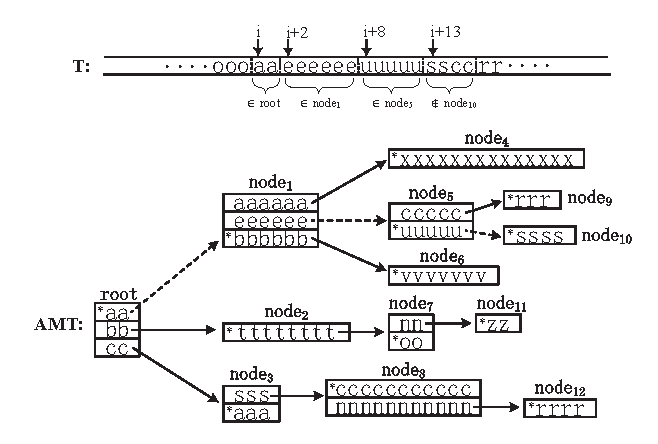
\includegraphics[width=0.75\textwidth]{figures/2_MPM/match}
  \caption{对文本串中潜在匹配位置 $i$ 的核实过程。}
  \label{fig:matching}
\end{figure}

接下来, 将给出一个实例来说明如何使用 \ref{subsec:amt} 节所构造的AMT,对
文本串 $T$ 中的潜在匹配位置 $i$ 进行核实。 核实过程起始于AMT的根节点:根
据 $key\_len(root)=2$, 将起始于位置 $i$ 的同样长度的文本子
串, 即 $T[i,\,2]=aa$, 与根节点中的键进行匹配。 由于 $aa \in
root$ 且 $aa$ 被标记为模式终止。 所以模式串 $T[i,\,2]=aa$
(即 $P$ 中的 $p_6$) 出现于位置 $i$。 接着, 核实过程将转移到 $root.aa$ 所
对应的孩子节点。

对于节点 $node_1$, 由于 $key\_len(node_1)=6$, 同样长度的子
串 $T[i+2,\,6]=e^6$ (跟随在 $T[i,\,2]$ 之后) 将会与 $node_1$ 中的键进行
匹配。 由于 $e^6 \in node_1$, 且并非模式串结尾, 核实过程将转移
到 $node_1.e^6$ 所对应的孩子节点 $node_5$ 上。

在节点 $node_5$ 上, 由于接下来的子文本串 $T[i+8,\,5]=u^5 \in
node_5$ 且 $u^5$ 被标记为模式终止, 另一个模式串 $T[i,\,13]=a^2e^6u^5$
(即 $P$ 中的 $p_4$) 被发现于 $i$。 然后,核实过程将转移到 $node_5.u^5$
所应的孩子节点 $node_{10}$ 中。

在 $node_{10}$ 上, 由于 $T[i+13,\,4]=sscc \notin node_{10}$, 对位
置 $i$ 的核实过程将终止。 接下来, 匹配引擎将转移到下一个位置 $i+1$, 同
时激活过滤模块。

从以上过程可以看到, 对潜在匹配位置的核实过程对应于AMT中的一条“核实路
径”, 其中的节点都参与过与文本串的比较。 本例中, 位置 $i$ 所对应的核实
路径为:
$root \rightarrow node_1 \rightarrow node_5 \rightarrow node_{10}$, 由
图 \ref{fig:matching} 中的虚线箭头表示。


\subsection{自适应地产生树节点}
\label{subsec:nodes}

如 \ref{subsec:amt} 节所说的, AMT中的每个节点都有其特定的索引结构用来保
存前缀集中的前缀。 索引结构的类型将根据前缀集的特性自适应地进行选择。 由
于前缀集中的所有前缀(键)都具有相同的长度, 前缀集的特性主要可以由两个参
数进行刻画,即前缀集所包含前缀(键)的长度和数量。 这两个参数分别
由 \ref{subsec:amt} 节中的 $lss$ 和 $ndp$ 来表示。

有三种不同的结构, 即字符映射表, 字符串数组及哈希表可以用来作为树节点来
存储具有不同 $lss$ 和 $ndp$ 的前缀集。 接下来,将详细讨论这几种节点结构。

\noindent\subsubsection{字符映射表}

给定前缀集, 如果其前缀长度都为1 ($lss=1$), 即每一个前缀都是单个字符, 则
选用空间高效的字符映射表(由 Leis \cite{Leis2013} 提出)作为树节点。 对于
不同的前缀数 (即 $ndp$, $1 \leq ndp \leq 256$),有四种不同容量的字符映
射表可供选择。

\begin{figure}[H]
  \centering
  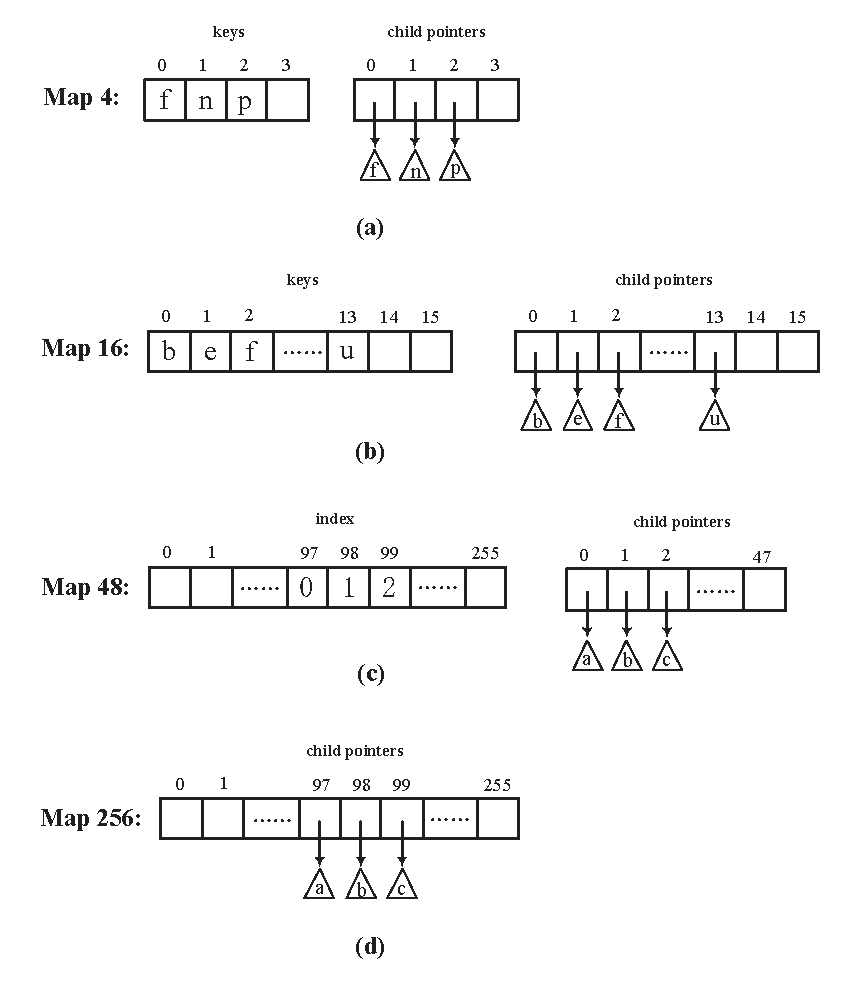
\includegraphics[height=5in, width=5in]{figures/2_MPM/character_map}
  \caption{四种不同容量的字符映射表。 三角形代表相应键的子节点。}
  \label{fig:character map}
\end{figure}

图 \ref{fig:character map} 显示了由其最大容量所命名的四种字符映射表。 字
符映射表的键和其所对应的孩子指针,分别存放于两个不同的数组中,而非使用
二元组 (\emph{键, 孩子指针}) 数组, 这样能在保证高效匹配的同时保持节点的
紧凑。

\begin{itemize}
\item \textbf{Map 4} (当 $1 \leq ndp \leq 4$ 时采用): 这种最小的字符映
  射表最多能存储4个键。 它使用4个元素的数组来存储键,用另一个同样长度的
  数组来存储孩子指针。 键及其所对应的孩子指针存储在各自数组的相同位置,
  键按照其ASCII码值顺序存储。 一旦目标字符在键数组中被找到, 其所对于的孩
  子指针可在另一个数组的同样位置找到。  图 \ref{fig:character map} (A)
  显示了包含了3键:$f$, $n$ 和 $p$ 的 Map 4 结构,其中包含了键的三角形
  表示对应的孩子节点。

\item \textbf{Map 16} (当 $5 \leq ndp \leq 16$ 时采用): 这种字符映射表
  可以存储5到16个键。 它与Map 4映射表有类似的结构, 但两个数组都扩大到
  了16个元素。 目标字符可由键数组上的二分查找进行快速检
  索。 图 \ref{fig:character map} (B) 显示了具有14个键的 Map 16 映射
  表。


\item \textbf{Map 48} (当 $17 \leq ndp \leq 48$ 时采用): 随着键数量的增
  加, 在键数组中查找目标字符将变得越来越耗时。 因此, 当键的数量超过16个
  (但小于49个)时,将不再显示地存储键, 而是使用一个具有256个元素的索引
  数组,该数组可由目标字符的ASCII码值作为下标直接访问其元素。 索引数组
  存储的是另外一个具有48个元素的孩子指针数组的索引(下标)(在$[0,47]$范
  围内的整数)。 相比直接存储孩子指针,这种方式更加节省空间, 因为每个数
  组下标只占用一个字节的空间。 图 \ref{fig:character map} (C) 显示了一
  个Map 48映射表, 其中字符 $a$, $b$, $c$ 的ASCII码值分别为 97, 98, 99。

\item \textbf{Map 256} (当 $49 \leq ndp \leq 256$ 时采用): 最大的字符映
  射表只包含一个具有256个元素的数组来直接存储孩子指针,其中每个元素被初
  始化为 $NULL$。 当键的数量在49到256之间时,采用该类型的映射表作为树节
  点。 对于Map 256映射表, 相应的孩子节点可直接通过目标字符的ASCII码值找
  到。 与其他类型的映射表不同, Map 256只包含一个数组, 因此无需进行数组
  的二次访问, 而且,如果所包含数组大部分元素非空, 该结构同样非常紧
  凑。 图 \ref{fig:character map} (D) 显示了一个Map 256映射表, 其中只有
  一个指针数组。
\end{itemize}

在类型为字符映射表的节点中搜索目标字符的具体操作由算
法 \ref{alg:character map} 给出。

\begin{algorithm}
  \caption{在类型为字符映射表的节点中进行搜索}
  \label{alg:character map}
  \begin{algorithmic}[1]
    \REQUIRE ~~\\
    类型为字符映射表的节点 $node$\\
    目标字符 $t\_ch$
    \ENSURE ~~\\
     $node.t\_ch$ 所对应的孩子节点 (可能为 $NULL$)。
    \STATE
    \STATE $count \leftarrow$ 字符映射表中的键的个数
    \STATE
    \SWITCH{字符映射表的类型}
    \CASE{\textsf{Map 4}}
    \FOR{$i \leftarrow 0$ to $count-1$}
    \IF{$keys[i]=t\_ch$}
    \RETURN $child\_pointers[i]$
    \ENDIF
    \ENDFOR
    \STATE 出现失配,返回 $NULL$
    \ENDCASE
    \STATE
    \CASE{\textsf{Map 16}}
    \STATE $low \leftarrow 0, high \leftarrow count-1$
    \WHILE{$low \le high$}
    \STATE $mid \leftarrow \lfloor (low+high)/2 \rfloor$
    \IF{$t\_ch=keys[mid]$}
    \RETURN $child\_pointers[mid]$
    \ELSIF{$t\_ch<keys[mid]$}
    \STATE $high \leftarrow mid-1$
    \ELSE
    \STATE $low \leftarrow mid+1$
    \ENDIF
    \ENDWHILE
    \STATE 出现失配,返回 $NULL$
    \ENDCASE
    \STATE
    \CASE{\textsf{Map 48}}
    \IF{$index[t\_ch] \neq NULL$}
    \RETURN $child\_pointers[index[t\_ch]]$
    \ELSE
    \STATE 出现失配,返回 $NULL$
    \ENDIF
    \ENDCASE
    \STATE
    \CASE{\textsf{Map 256}}
    \RETURN $child\_pointers[t\_ch]$
    \ENDCASE
    \ENDPWITCH
  \end{algorithmic}
\end{algorithm}

\subsubsection{字符串数组}
\label{sec:string array}

对于键长大于1 (即 $lss > 1$) 且键数不超过100 (即 $ndp \leq 100$)的前缀
集, 将选用字符串数组作为树节点来存储其中的键。 类似于 Map 4 和 Map 16 结
构, 键按照字典序存储在一个大小为 $ndp \times lss$ 字节的数组中, 每个键
占用 $lss$ 字节。 孩子指针存储在另一个数组的对应位置
上。 图 \ref{fig:string array} 显示了包含了3个键: $aaa$, $bbb$ 和 $ccc$
的字符串数组结构。

\begin{figure}[H]
  \centering
  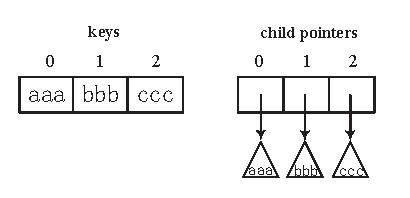
\includegraphics[width=0.45\textwidth]{figures/2_MPM/string_array}
  \caption{包含3个键 $aaa,\, bbb,\, ccc$ 的字符串数组结构。}
  \label{fig:string array}
\end{figure}

为了高效起见, 如果键的数量小于5个, 则在键数组上使用简单的线性查找算法来
搜索目标字符串; 否则, 将采用更高效的 (也更为复杂的) 二分查找算
法。 算法 \ref{alg:string array} 显示了在类型为字符串数组的节点中搜索目
标字符串的过程,其中 $A \prec B$ 表示字符串 $A$ 以字典序小于字符
串 $B$。 对于包含小于5个键的字符串数组, 目标字符串将按顺序与键数组中的元
素依次比较。 如果目标字符串匹配了某个键, 返回指针数组中对应位置所包含的
孩子节点指针; 否则, 将出现失配。 另一方面, 如果键的数量大于4, 将使用二分
查找算法从键数组的中间元素开始, 搜索目标字符串。

\begin{algorithm}
  \caption{在类型为字符串数组的节点中搜索}
  \label{alg:string array}
  \begin{algorithmic}[1]
    \REQUIRE ~~\\
    类型为字符串数组的节点 $node$ \\
    目标字符串 $t\_str$\\
    \ENSURE ~~\\
     $node.t\_ch$ 所对应的孩子节点 (可能为 $NULL$)\\
    \STATE
    \STATE $count \leftarrow$ 节点 $node$  所包含的键数
    \STATE
    \IF{$count < 5$}
    \STATE $i \leftarrow 0$
    \WHILE{$i < count$ 且 $keys[i] \prec t\_str$}
    \STATE $i \leftarrow i+1$
    \ENDWHILE
    \IF{$i < count$ 且 $keys[i]=t\_str$}
    \RETURN $child\_pointers[i]$
    \ELSE
    \STATE 出现失配,返回 $NULL$
    \ENDIF
    \ELSE
    \STATE $low \leftarrow 0$, $high \leftarrow count-1$
    \WHILE{$low \leq high$}
    \STATE $mid \leftarrow \lfloor (low+high)/2 \rfloor$
    \IF{$t\_str = keys[mid]$}
    \RETURN $child\_pointers[mid]$
    \ELSIF{$t\_str < keys[mid]$}
    \STATE $high \leftarrow mid - 1$
    \ELSE
    \STATE $low \leftarrow mid + 1$
    \ENDIF
    \ENDWHILE
    \STATE 出现失配,返回 $NULL$
    \ENDIF
  \end{algorithmic}
\end{algorithm}

\subsubsection{哈希表}
\label{sec:hash table}

对于键数大于100的前缀集 (即 $lss > 1$ 且 $ndp > 100$), 即使在字符串数组
上使用二分查找算法也不够高效。 此时, 将采用一种更快 (也更大)的数据结
构 --- 哈希表, 来处理包含大量键的情况。 值得注意的是, 哈希表是直接基于后
缀集构建的, 而不是像其他节点结构那样基于(从后缀集中生成的)的前缀集。 在
我们的实现中, 哈希表是一个孩子指针数组, 其中所有元素初始化为 $NULL$, 同
时, 配合使用一个字符串哈希函数, 该函数能将字符串转化为正整数。

具体地说, 给定后缀集 $SF$, 哈希表的长度(即元素个数, 由 $table\_size$ 表
示) 由 $ndp$ 和一个给定的负载因子 $lf$
(即 $ndp$ 与 $table\_size$ 比值) 决定, 即。
$table\_size = \lceil ndp\,/\,lf \rceil$。 例如, 给定 $ndp =
1000$ 及 $lf = 70\%$, 则哈希表的长度为
$table\_size = \lceil 1000/0.7 \rceil = 1429$。 注意, 这里的 $ndp$ 被定
义为后缀集 $SF$ 中, 后缀所包含的长为 $lss$ 的不同前缀的数量, 这与去重后
的前缀集 $PF$ 所包含的前缀数相同。

算法 \ref{alg:hash} 显示了基于后缀集 $SF$ 构建哈希表的过程。  首先,
$SF$ 将会基于哈希值被分为若干个子后缀集: 对于每个后缀 $suf \in SF$, 它
的前缀 $suf^{+lss}$ 将通过哈希函数转化为一个 0 到 $table\_size-1$ 之间
的整数 $i$, 然后 $suf$ 将与哈希表第 $i$ 个元素相关联。 此后, 那些长
为 $lss$ 的前缀被哈希到同一个值的后缀将与哈希表的同一个元素相关联, 构成
一个子后缀集。 接着, 为了解决哈希冲突, 对于哈希表中每个非 $NULL$ 元素所
关联的子后缀集 $SSF$, 构造其相应的前缀集, 然后按照算
法 \ref{alg:amt} 中 \textbf{while} 循环所示, 构造相应的树节点。 新产生的
树节点将会取代子后缀集与相应的哈希表元素关联。 这样, 会有许多不同结构的
节点关联到同一个哈希表上。

\begin{algorithm}
  \caption{构建哈希表}
  \label{alg:hash}
  \begin{algorithmic}[1]
    \REQUIRE ~~\\
    后缀集 $SF$ 及负载因子 $lf$ \\
    \ENSURE ~~\\
    哈希表\\
    \STATE
    \STATE $ndp \leftarrow$ $SF$ 中, 后缀所具有的长为 $lss$ 的不同前缀
    的数量
    \STATE $table\_size \leftarrow \lceil ndp\,/\,lf \rceil$
    \STATE $hash\_table \leftarrow$ 产生一个具有
    $table\_size$ 个孩子指针的数组, 每个指针被初始化为 $NULL$
    \STATE
    \FOR{每一个 $suf \in SF$}
    \STATE $i \leftarrow Hash(suf^{+lss})$
    \STATE 将 $suf$ 与 $hash\_table[i]$ 相关联
    \ENDFOR
    \STATE
    \FOR{$i \leftarrow 0$ to $table\_size - 1$}
    \IF{$hash\_table[i]\, \neq\, NULL$}
    \STATE $SSF \leftarrow \{suf\,|\,suf\in SF\; and\; Hash(suf^{+lss})=i\}$
    \STATE $new\_node \leftarrow$ 如算法 \ref{alg:amt} 中的
    \textbf{while} 循环所示, 基于 $SSF$ 自适应地产生一个树节点
    \STATE 将 $new\_node$ 与 $hash\_table[i]$ 相关联
    \ENDIF
    \ENDFOR
    \STATE
    \RETURN $hash\_table$
  \end{algorithmic}
\end{algorithm}

给定长为 $lss$ 目标字符串, 首先计算其哈希值并将哈希值用作哈希表的数组下
标。 如果哈希表对应元素为 $NULL$, 意味着出现失配, 将终止核实过程并转移到
文本的下一个位置; 否则, 核实过程将转移到与其关联的孩子节点中。

哈希表所采用的字符串哈希函数, 将会很大程度地影响匹配的效率。 在我们的实
现中, 对于每一次匹配任务, 将从一个哈希函数族 $H$ 中随机地选取一个哈希函
数。 所采用的哈希函数来自于 Ramakrishna \cite{Ramakrishna1997} 所提出
的 \emph{shift-add-xor} 哈希函数族, 该哈希函数族具有良好的均匀性和一致
性。

\subsection{进一步优化}
\label{sec:further improments}

以上介绍的核实模块已经相当高效, 但是仍然有一些技术可以进一步提升其时间
和空间效率。\\

1. 分解AMT

以上介绍的核实模块基于由整个模式集所构建的AMT。 事实上, 可以将大的AMT分
解为多个小AMT, 同时让每一次核实操作只关联其中一个小AMT, 这样可以进一步
提高核实过程的效率。 分解过程基于以下思路。

如 \ref{sec:filter} 所述, 过滤过程基于滑动窗口所包含子串末尾的 $k$ 字符
块。 对于文本串 $T$ 的一个位置 $i$, 若某个模式串 $p_j$ 出现于 $i$, 则一
定有 $Hash[T[i+lss-k,k]] = Hash[p_j[lss-k+1,k]]$
($Hash[p_j[lss-k+1,k]]$ 被称为 $p_j$ 的标签值)。 这意味着,可以根据标签
值将模式串进行分组:具有相同标签值的模式串被分成一组,构成一个子模式
集。 然后,为每一个子模式集构造一棵(小的)AMT。 另外, 还需构建一个索引表
使得相应的AMT可以由其对应的标签值在 $O(1)$ 时间内找到。 这样, 核实模块将
包含一个索引表和若干个(小的)AMT。

在过滤阶段, 一旦 $T$ 中的一个潜在匹配位置 $i$ 被找到, 将计算哈希
值 $Hash[T[i+lss-k,k]]$ 并将其用作索引表的索引来找到对应的AMT。 由于
该AMT的规模相比之前减小了,核实所用的时间也会相应地减少。\\

2. 节点合并

类似于Trie树结构中广泛使用的路径压缩技术,在AMT中的一条路径上,所有只包
含一个键的节点可以合并为一个节点。 该技术可以从时间和空间两方面提
高AMT的效率。
为了说明该技术的优势,考虑模式集$P=\{p_1=e^6u^5sscc,\; p_2=e^6u^5,\;
p_3=e^6\}$ 和其所对应的AMT。 如图 \ref{fig:merge} 所示, 所构建
的AMT包含3个节点, 每个节点都只有一个键。 在 $x86\_64$ 体系结构中, 这种实现
方法大致需要55字节的存储空间:存储3个键需要15字节, 2个孩子指针需要16字
节, 3个指向各自匹配函数的函数指针需要24字节。 然而, 如果将3个键连接
成1个字符串, 这3个节点便可合并为1个, 这样不仅不再需要孩子指针,指向匹配
函数的指针也从3个减少为1个。合并后的节点构成一种新的节点结构,有别
于 \ref{subsec:nodes} 节介绍的几种节点类型。

\begin{figure}[H]
  \centering
  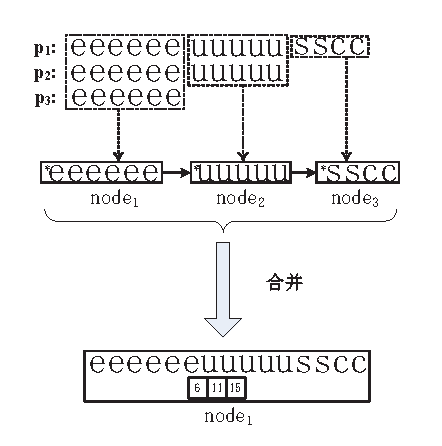
\includegraphics[height=3in, width=3in]{figures/2_MPM/node_merge}
  \caption{节点合并。}
  \label{fig:merge}
\end{figure}

对于合并后的节点, 唯一的问题是如何区分被连接在一起的键。 为此, 需要使
用一个长度数组来记录每个键的长度,其中每个数组元素占用一个字节 (使用
$unsigned char$ 类型)。 通过每个键的长度,便可以识别出每个键,这样,在
合并后的节点中搜索目标字符串就变的很容易。

综上, 在节点合并之后, AMT只包含一个合并后的节点,且只占用26字节的存储空
间 (15个字节用来存储键, 3个字节用来存储长度数组, 8个字节用来存储指向匹
配函数的指针), 这样, 相比原先的AMT,合并节点后的AMT可以节省29个字节的存
储空间。 另外, 只需要一次随机访问内存便可以取出需要的节点, 相比原先需
要三次访问内存来取得需要的节点, 减少了内存访问量,提高了匹配速度。\\

3.节点分裂

为了进一步提高节点的匹配效率, 一旦某个节点所包含的键具有公共前缀, 该前
缀便可以从节点中分离出来形成一个(包含单个键的)新节点。 (由于被分离出的
前缀是一个字符串或字符,新节点的结构只能是Map 4字符映射表或字符串数
组)。 在一个节点上搜索目标串时,节点分割技术可以大幅减少不必要的比较操
作。 例如, 如图 \ref{fig:split} 所示, 考虑在一个类型为字符串数组的节点
中搜索目标字符串 $a^5u$, 节点中的4个键具有公共前缀 $a^5$。 根据算
法 \ref{alg:string array}, 目标字符串需要与这4个键依次进行逐字符比较才
能确认其是否匹配某个键,这总共需要 $6 \times 4 = 24$ 次比较操作。 然而,如
果公共前缀 $a^5$ 被分离出来并形成一个新的节点,如图 \ref{fig:split} 所
示, 对于同样的目标字符串, 只需要9次字节比较操作便可以最终确
认 ($node_1$ 上需要5次比较, $node_2$ 上需要4次比较)。 很明显, 通过对原
先的节点进行分割,减少了15次比较操作。

\begin{figure}[H]
  \centering
  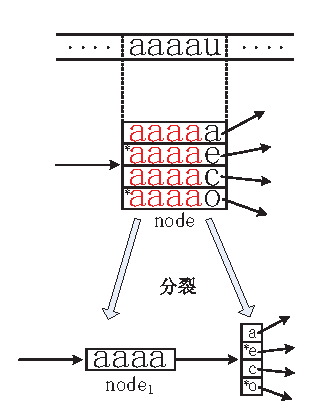
\includegraphics[height=2.8in, width=2.6in]{figures/2_MPM/node_split}
  \caption{节点分裂。}
  \label{fig:split}
\end{figure}

\section{实验结果}
\label{sec:2_experiments}

在本节中, 我们将所提出的匹配引擎(Fast Engine for MPM, 简称
为\textsf{FEMPM}) 与其他5个算法进行比较,来评估匹配引擎的性能。 参与比
较的算法包括: 2个经典的MPM基准算法 \textsf{AC} 和 \textsf{WM} ; 3个近
期提出的高效算法 \textsf{Split},
\textsf{MASM} 及 \textsf{Pre-filter+AC}。 所有算法都从两个方面对其性能进
行评估: 通过具有不同 $lsp$ 的模式集,来测试算法的鲁棒性;通过包含不同数
量模式的模式集来测试算法的可伸缩性。

\subsection{实验设置}


实验在一台PC上进行,配置有 Intel core i7 2.93GHz CPU, 8GB 内存 和 1TB硬
盘, 操作系统为GNU/Linux。 所有算法以 C/C++ 实现, gcc编译(-O2)。 测试数
据为来自于 Pizza\;\&\;Chili 语料库 (http://pizzachil.dcc.uchile.cl) 的
真实英文文本。 模式串从文本串中随机抽取,构成模式集。

实验过程中, \textsf{FEMPM} 的参数设置如下: 对于字符串数组, 如果其包
含的键数大于4, 则在键数组上使用二分查找来搜索目标字符串; 否则, 将使用
简单的线性查找算法 (对于包含小于4个键的字符串数组,线性查找算法由于其简
单性,反而更加高效)。 对于哈希表, 为了平衡时间效率和空间效率,负载因子被
设置为 {0.5}; 产生哈希函数的种子值在 1~50 间随机产生; 左移值 L 和右移
值 R 分别被设置为 \textbf{2} 和 \textbf{6} (有关哈希函数的参数都选
自 \cite{Ramakrishna1997})。 一旦 $ndp$ 大于 \textbf{100}, 将选用哈希表
来取代字符串数组作为节点结构。 所有这些选择的参数都在大量模式集上进行了
广泛的实验,在实际中被证实是高效的。

\subsection{鲁棒性评估}

正如前面提到过的, 许多MPM算法对于模式集的最短模式串长(即$lsp$)非常敏
感。 所以,有必要测试 \textsf{FEMPM} 引擎和其它算法在具有不同 $lsp$ 模式
集下的鲁棒性。 共有9个模式集参与测试,其 $lsp$从2递增到10,每个模式集都
包含$10^5$个模式串。 文本串的大小固定为 200 MB。 测试模式集的特征在
表 \ref{tab:lsps} 中列出, 包括: 最短模式串长 (LSP), 最长模式串
长 (LLP), 模式串的平均长度 (ALP), 模式串长的标准差 (SD), 模式串总
长 (TLP) 和模式串的数量 (Count)。

\begin{figure}[H]
  \centering
  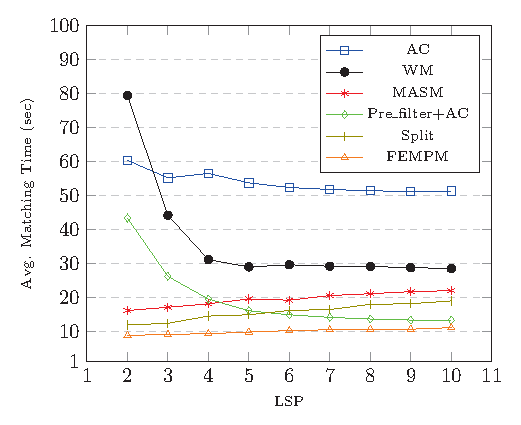
\includegraphics[height=3in, width=3.2in]{figures/2_MPM/lsp}
  \caption{测试算法在具有不同lsp模式集下的匹配时间。}
  \label{fig:lsp}
\end{figure}


\begin{table}
  \centering
  \topcaption{测试模式集的特性。}
  \label{tab:lsps}
  \begin{tabular}{ccccccc}
    \hline
    Pattern Set & LSP  & LLP  & ALP & SD & TLP & Count\\
    \hline
    $P_1$ & 2 & 50 & 25.9 & 14.1 & 2,599,020 & $10^5$\\
    $P_2$ & 3 & 50 & 26.5 & 13.9 & 2,646,762 & $10^5$\\
    $P_3$ & 4 & 50 & 27.0 & 13.6 & 2,704,091 & $10^5$\\
    $P_4$ & 5 & 50 & 27.6 & 13.2 & 2,745,545 & $10^5$\\
    $P_5$ & 6 & 50 & 27.9 & 13.0 & 2,793,178 & $10^5$\\
    $P_6$ & 7 & 50 & 28.4 & 12.7 & 2,843,580 & $10^5$\\
    $P_7$ & 8 & 50 & 29.0 & 12.4 & 2,903,343 & $10^5$\\
    $P_8$ & 9 & 50 & 29.5 & 12.1 & 2,948,372 & $10^5$\\
    $P_9$ &10 & 50 & 30.0 & 11.8 & 2,998,992 & $10^5$\\
    \hline
  \end{tabular}
\end{table}


图 \ref{fig:lsp} 给出了每个测试算法在独立运行5次后的平均运行时间(以秒位
单位)。 总体来说, \textsf{AC} 算法受 $lsp$ 变化的影响不大。 但是, 其所构
建的DFA会消耗大量存储空间。 更糟糕的是, 算法在运行过程中会进行大量且不
可预测的状态转移,这会造成严重的cache miss,从而影响算法性能。 另一方
面, 同样基于DFA的 \textsf{Split} 算法, 对 $lsp$ 的变化也不敏感, 而且由
于它从模式集中抽取了一个子集来构造DFA,同时使用了位分割技术, 使其空间和
时间消耗都有大幅下降。 由图 \ref{fig:lsp} 可以看出,\textsf{WM} 算法的性
能受 $lsp$ 变化的影响很大: 对于 $lsp > 2$ 时,其性能优于AC, 但是对于包
含极短模式的模式集($lsp=2$),WM算法的性能将严重下降。 这是由于WM算法所
用的跳转策略并不适用于包含很短模式串的模式集,这意味着文本串中大部分位
置都无法被略过,而需要通过WM算法的哈希表进行二次检查,这将花费大量的时
间。  \textsf{Pre-filter+AC} 算法对于 $lsp > 5$ 的模式集的性能优于除
了 \textsf{FEMPM} 之外的其它算法。 该算法使用了类似的跳转策略: 一旦文本
串中的某个位置被Pre-filter过滤掉了, 其后最多有$lsp-1$个位置可以被跳
过。 因此, 对于 $lsp$ 较小的模式集, 文本中的大部分位置都无法被跳过, 这会
严重影响算法性能。 相比之下, \textsf{MASM} 算法对于较小 $lsp$ ($lsp
\leq 4$) 的模式集表现良好。 该算法首先通过前缀树结构对模式集进行压缩: 如
果模式串 $A$ 是另外一个模式串 $B$ 的前缀, $A$ 便可以合并到 $B$ 中。 然后,
算法将基于字典序为压缩后的模式集构造一棵二叉查找树。 相比长模式串, 短模
式串更有可能成为其它模式的前缀,因此, 更有可能被合并到其它串中。 因此,拥
有较小 $lsp$ 的模式集能被更好的压缩, 使得算法在匹配阶段的效率更高。

从图 \ref{fig:lsp} 可以看出, 我们所提出的 \textsf{FEMPM} 匹配引擎,对于
任何 $lsp$ 都拥有最佳的性能。 相比 \textsf{AC}, 对所有 $lsp$,匹配时间
平均减少了 $85\%$; 与更加高效的\textsf{Pre-filter+AC} 算法相比, 对于中
等长度的 $lsp$ ($lsp \geq 4$) 匹配时间减少了 $10\% \sim 20\%$, 对于较
小的 $lsp$ ($lsp < 4$), 匹配时间减少了 $70\%$。 尽管 \textsf{FEMPM} 的
过滤模块(和\textsf{Pre-filter+AC}类似), 同样不适用于较小的 $lsp$, 然而
其核实模块(即AMT), 相比 \textsf{Pre-filter+AC}的要更加高效。 这主要是由
于AMT节点的自适应性, 使得对于任何 $lsp$,所构造的AMT都能根据模式集的特
性自适应地调整到最优结构。得益于此, \textsf{FEMPM} 对于所有的测试模式集
都有最好的鲁棒性。 表 \ref{tab:node types} 中列出了不同模式集对应AMT中
节点类型的统计信息。 其中 Map 1 和 String Array 1结构分别是 Map
4 和String Array结构只包含一个元素的特殊情形。 由此可以看出, 随着模式
集 $lsp$ 的变化, 对应AMT中的节点类型也会发生很大变化,这反映了AMT的自适
应性。

再者, \textsf{FEMPM} 的性能非常稳定可靠。 一旦文本的长度和模式串的数量确
定, 算法的运行时间对于不同 $lsp$ 的模式集,变化很
小。 如图 \ref{fig:lsp} 所示, 给定大小为200MB的文本和$10^5$个模式串,对
于不同的 $lsp$, \textsf{FEMPM} 的匹配时间大致都保持
在10s左右; 当 $lsp$从2递增到10时, 匹配时间的变化不超过2s。 事实
上, 随着$lsp$ 的增加, AMT中从根节点到叶节点路径的平均长度将会轻微地增
加。 相应地, 对于文本串中的某些位置,其对应的核实路径会增长,这会轻微地
影响算法的速度。

\begin{table}[!h]
  \centering
  \footnotesize
  \topcaption{不同lsp模式集所对应AMT的节点类型统计。}
  \label{tab:node types}
  \begin{tabular}{cccccccccc}
 \hline
 Lsp &
 Map 1 &
 Map 4 &
 Map 16 &
 Map 48 &
 Map 256 &
 String Array 1&
 String Array   &
 Hash Table &
 Total\\
 \hline
 2  & 2,464 & 2,096 & 663 & 133 & 0 & 63,274 &  21,627 & 10 & 90,267\\
 3  & 2,379 & 1,636 & 385 & 90  & 0 & 64,701 &  22,551 & 10 & 91,752\\
 4  & 2,273 & 1,329 & 201 & 57  & 0 & 66,162 &  22,736 &  1 & 92,759\\
 5  & 2,045 & 1,104 & 112 & 45  & 0 & 68,152 &  22,048 &  1 & 93,507\\
 6  & 1,758 &   899 &  52 & 34  & 0 & 70,179 &  20,818 &  1 & 93,741\\
 7  & 1,560 &   807 &  29 & 33  & 0 & 72,284 &  19,280 &  1 & 93,994\\
 8  & 1,515 &   803 &  20 & 31  & 0 & 73,447 &  18,274 &  1 & 94,091\\
 9  & 1,441 &   788 &  24 & 30  & 0 & 74,584 &  17,120 &  1 & 93,988\\
10  & 1,361 &   794 &  24 & 29  & 0 & 75,094 &  16,427 &  1 & 93,730\\
\hline
  \end{tabular}
\end{table}

\subsection{伸缩性评估}

本节将评估各种算法在不同容量模式集下的可伸缩性。 和前面一样, 文本串被固
定为200MB, 有两组模式集用于测试。 其中较小的一组包含9个模式集, 对应的模
式串数量由$1 \times 10^5$ 增加到 $9 \times 10^5$, 每次的增幅
为 $10^5$, 而较大的一组包含10个模式集, 对应模式串的数量由$10^6$ 增加
到 $10^7$,每次增加 $10^6$。 所有模式集的串长变化范围固定为 $5 \sim
50$。


\begin{figure}[H]
  \centering
  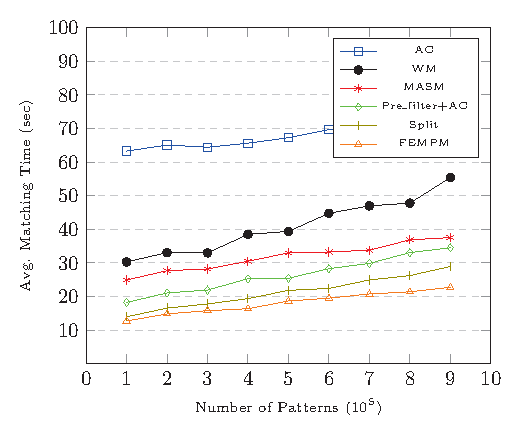
\includegraphics[height=3in, width=3.2in]{figures/2_MPM/small_group}
  \caption{测试算法对于较小一组模式集的平均运行时间。}
  \label{fig:small_group}
\end{figure}

对于较小的一组模式集, 每个测试算法在每个模式集上独立运行5次,其平均运行
时间如图 \ref{fig:small_group} 所示。 实验结果表明, 随着模式串数量的增
加,AC算法的性能较为稳定(虽然不高),但由于内存溢出,AC算法无法处理规模
超过 $7 \times 10^5$ 的模式集。 \textsf{WM} 算法尽管在性能上优
于 \textsf{AC}, 但其表现却不稳定。 例如, 当模式串数量从$2 \times 10^5$
增加到 $3 \times 10^5$时, WM算法的匹配时间仅增加了1s,然而当模式串数量
由 $8 \times 10^5$ 增加到 $9 \times 10^5$时, 匹配时间却增加了9s。 因此,
我们无法根据模式集的规模来预测其运行时间。 \textsf{Pre-filter+AC} 算法
对模式集规模的增长表现良好, 但其运行时间依然无法预测。比如,当模式集规
模从 $4 \times 10^5$ 增加到 $5 \times 10^5$ 时,其运行时间几乎不变。 这
主要是因为,两个算法所使用的过滤器,其效果高度依赖于文本串和模式串本身
的内容,对于某些模式集,若其所包含的模式串频繁出现于文本中, 过滤器的效
果将大打折扣。 另一方面, 随着模式串数量的增长, \textsf{MASM} 算法的匹配
时间,比 \textsf{Pre-filter+AC} 算法增长地更慢, 这主要是由
于 \textsf{MASM} 算法的匹配时间主要依赖于其所构建的二叉查找树的深
度, 这个深度随着模式集规模的增长而增加地非常缓慢。 \textsf{Split} 算法
对于规模不大的模式集表现非常良好, 它只比 \textsf{FEMPM} 引擎慢了 $10\%
\sim 20\%$。


\begin{table}[!htp]
  \centering
  \footnotesize
  \topcaption{较小一组模式集所对应AMT的节点类型统计。}
  \label{tab:small}
  \begin{tabular}{cccccccccc}
 \hline
 Size &
 Map 1 &
 Map 4 &
 Map 16 &
 Map 48 &
 Map 256 &
 String Array 1&
 String Array   &
 Hash Table &
 Total\\
\hline
$1 \times 10^5$ &  2,000 &  1,006 &    72 &  18 & 0 &  68,268 &  21,971 & 103 &  93,438 \\
$2 \times 10^5$ &  4,628 &  2,808 &   307 &  42 & 0 & 130,440 &  46,514 & 244 & 184,983 \\
$3 \times 10^5$ &  7,414 &  4,858 &   574 &  84 & 0 & 190,653 &  71,757 & 403 & 275,746 \\
$4 \times 10^5$ & 10,555 &  7,282 &   946 & 139 & 0 & 247,656 &  97,967 & 544 & 365,089 \\
$5 \times 10^5$ & 13,703 & 10,651 & 1,503 & 238 & 4 & 302,350 & 124,528 &  17 & 452,994 \\
$6 \times 10^5$ & 17,335 & 13,536 & 1,954 & 298 & 0 & 356,644 & 151,435 &  31 & 531,233 \\
$7 \times 10^5$ & 21,080 & 16,872 & 2,405 & 388 & 4 & 408,165 & 179,621 &  35 & 628,570 \\
$8 \times 10^5$ & 24,357 & 20,094 & 2,977 & 436 & 3 & 457,674 & 208,426 &  37 & 714,004 \\
$9 \times 10^5$ & 28,356 & 23,924 & 3,441 & 513 & 9 & 504,779 & 238,632 &  42 & 799,696 \\
\hline
  \end{tabular}
\end{table}

在所有测试算法当中, \textsf{FEMPM} 引擎都是最为高效且稳定
的。 \textsf{FEMPM} 的高性能主要来自于AMT的根节点:当模式串数量增加,根
节点的类型几乎总是哈希表。 如前所述, 根节点充当了二次过滤器的角色,对于
大量的无法由过滤模块过滤的文本位置,都有机会被根节点过滤掉。 另外, 模式
串数量的增加,主要导致AMT宽度的增加而非其深度。 因此, 对于文本串中的每
一个位置, 匹配时间变化很小。 依据实验结果, 我们甚至可以根据模式集的规模,
来粗略地估计\textsf{FEMPM}的运行时间: 给定 200 MB 文本串, 模式串数量每
增加 $10^5$, 算法将会多增加1s的匹配时间。 AMT中的节点类型统计信息如
表 \ref{tab:small} 所示。 可以看到,每增加 $10^5$ 个模式串,相应的AMT中
会多产生 $9 \times 10^4$ 个树节点。

\begin{figure}[H]
  \centering
  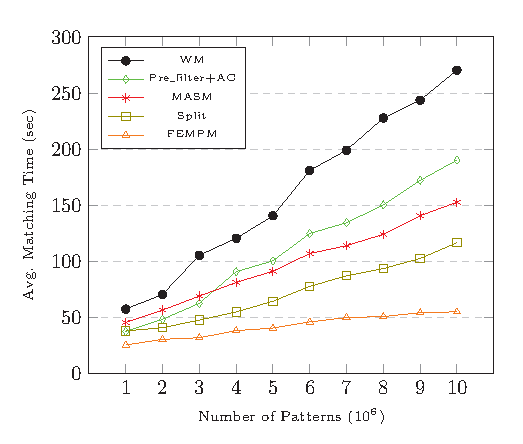
\includegraphics[height=3in, width=3.2in]{figures/2_MPM/large_group}
  \caption{测试算法对于较大一组模式集的平均运行时间。}
  \label{fig:large_group}
\end{figure}

对于较大一组模式集, 测试算法的平均运行时间如图 \ref{fig:large_group} 所
示。 可以看到, 随着模式串数量由 $10^6$ 增加到 $10^7$, 每个测试算法的匹配
时间增幅分别为: $410\%$ (\textsf{WM}), $374\%$
(\textsf{Pre-filter+AC}), $238\%$ (\textsf{MASM}), $191\%$
(\textsf{Split}), $112\%$ (\textsf{FEMPM})。 每增加 $10^6$ 个模式串, 测
试算法的匹配时间的平均增加量分别为: $23.7s$ (\textsf{WM}), $17.0s$
(\textsf{Pre-filter+AC}), $12.3s$ (\textsf{MASM}),
$8.8s$(\textsf{Split}), $3.5s$ (\textsf{FEMPM})。 由此可见,
\textsf{Pre-filter+AC} 和 \textsf{WM} 算法对于较大规模的模式集表现不
佳。 这是因为, 随着模式串数量的增加, 文本串中每个位置匹配到某个模式串的
概率就会增加,这会减少过滤器的效果,导致算法性能下降。 \textsf{MASM}算
法在模式集规模大于$3 \times 10^6$时,优于 \textsf{Pre-filter+AC} 算法,
这主要归功于其所采用的模式集压缩技术和流水线化的二叉查找树良好的伸缩
性。 \textsf{Split} 算法相比其它算法 (除了 \textsf{FEMPM}) 具有更好的伸
缩性, 因为它只是从模式集中选取了一个子集(其中的每个模式串都不是其它任何
模式串的后缀)来构造DFA。

\begin{table}[!htp]
  \centering
  \footnotesize
  \topcaption{较大一组模式集所对应AMT的节点类型统计。}
  \label{tab:large_group}
  \begin{tabular}{cccccccccc}
 \hline
 Size &
 Map 1 &
 Map 4 &
 Map 16 &
 Map 48 &
 Map 256 &
 String Array 1&
 String Array   &
 Hash Table &
 Total\\
\hline
$1 \times 10^6$ &  38,935 &   27,428  &   6,468 &     851   &    4 &    588,343  &    240,886 &  1,027 &    903,942  \\
$2 \times 10^6$ &  85,900 &   68,973  &  17,084 &   2,141   &   20 &  1,091,527  &    496,001 &  2,015 &  1,763,661  \\
$3 \times 10^6$ & 136,054 &  117,527  &  28,092 &   3,410   &   17 &  1,547,659  &    764,359 &  2,749 &  2,599,867  \\
$4 \times 10^6$ & 189,926 &  171,155  &  40,328 &   4,716   &   23 &  1,966,326  &  1,045,558 &  3,450 &  3,421,482  \\
$5 \times 10^6$ & 247,707 &  230,163  &  83,043 &   5,989   &  38 &  2,354,308   &  1,332,896 &  3,885 &  4,228,029  \\
$6 \times 10^6$ & 304,863 &  293,591  &  65,475 &   7,169   &   49 &  2,706,094  &  1,625,261 &  4,379 &  5,006,881  \\
$7 \times 10^6$ & 366,861 &  361,695  &  77,899 &   8,434   &   53 &  3,030,673  &  1,925,027 &  4,733 &  5,775,380  \\
$8 \times 10^6$ & 429,121 &  433,708  &  90,280 &   9,660   &   62 &  3,336,765  &  2,226,879 &  5,070 &  6,531,545  \\
$9 \times 10^6$ & 494,278 &  509,992  & 102,402 &  10,833   &   72 &  3,623,407  &  2,537,413 &  5,224 &  7,283,621  \\
$1 \times 10^7$ & 558,241 &  591,455  & 115,012 &  11,922   &   79 &  3,986,683  &  2,847,277 &  5,505 &  8,026,174  \\
\hline
\end{tabular}
\end{table}

相比之下, 对于规模较大的模式集, \textsf{FEMPM} 在所有测试算法中都是最
高效的。 模式串数量每增加 $10^6$, 匹配时间仅增加2.8s多, 这主要得益
于AMT优秀的可伸缩性,使得匹配时间随着模式串数量的增加而增长地非常缓
慢。 对于较大组模式集所对应的AMT,其节点类型统计信息如
表 \ref{tab:large_group} 所示。 其中,模式串数量每增加 $10^6$,AMT中只增
加大约 $8 \times 10^5$个节点。

\section{本章小结}
\label{sec:2_conclusion}

本章中,我们提出了一种快速的多模式匹配引擎 \textsf{FEMPM}。 引擎由过滤模
块与核实模块组成。 过滤模块主要用于过滤掉文本串中的非匹配位置, 而核实模
块则用于核实潜在的匹配位置。 核实模块基于一种被称为自适应匹配树的数据结
构, 它可以根据模式集的特性, 自适应的调整其内部节点结构, 使其具有良好的
鲁棒性和伸缩性。 得益于此, \textsf{FEMPM} 可以很好的应用于大规模模式匹配
问题。 未来, 我们将研究更加高效的节点结构。


% \begin{abstract} The Suffix Array (SA) is a fundamental data structure
% which is widely used in the applications such as string matching, text
% index and computation biology, etc. How to sort the suffixes of a string in
% lexicographical order is a primary problem in constructing SAs, and
% one of the widely used suffix sorting algorithms is
% \emph{qsufsort}. However, \emph{qsufsort} suffers one critical
% limitation that the order of suffixes starting with the same $2^k$
% characters can not be determined in the $k$-th round. To this point,
% in our paper, an efficient suffix sorting algorithm called
% \emph{dsufsort} is proposed by overcoming the drawback of the
% \emph{qsufsort} algorithm. In particular, our proposal maintains the
% \emph{depth} of each unsorted portion of SA, and sorts the suffixes
% based on the \emph{depth} in each round. By this means, some suffixes
% that can not be sorted by \emph{qsufsort} in each round can be sorted
% now, as a result, more sorting results in current round can be
% utilized by the latter rounds and the total number of sorting rounds
% will be reduced, which means \emph{dsufsort} is more efficient than
% \emph{qsufsort}. The experimental results shows the effectiveness of
% the proposed algorithm, especially for the text with high repetitions.
% \end{abstract}

\chapter{一种高效的后缀排序算法}
\label{chap:SS}


\section{引言}
\label{sec:3_introduction}

如何将给定字符串的所有后缀按照字典序进行排序, 是构建后缀数组的主要问
题。 目前, \emph{qsufsort}\cite{Larsson2007} 算法是解决该问题广泛使用的
算法之一。 该算法采用“前缀倍增”技术对后缀进行逐轮排序, 每一轮的排序将
基于上一轮的结果, 直到所有后缀都处于正确的字典序。 具体地, 首先所有后缀
将根据其首字符进行排序, 然后在每一轮中, 排序所依据的字符数将翻
倍, 这样, 在第\emph{k}轮之后, 所有后缀将根据其前 $2^{k}$ 个字符进行排
序。 这也意味着, 对于那些前$2^{k}$字符相同的后缀, 它们的次序无法在
第$k$轮之后被确定。 因此, 对于那些具有较大 \emph{LCP}(Length of the
Longest Common Prefix)的后缀, \emph{qsufsort} 需要许多轮才能确定它们的
次序, 这会严重影响算法效率。

为了克服 \emph{qsufsort} 的这种缺陷, 在本章中, 将提出一种基
于 \emph{qsufsort} 算法的改进的后缀排序算法--\emph{dsufsort}。 其核心思
想在于, 对后缀数组SA中每一个还未排序的部分(称作一个“桶”(bucket)),
\emph{dsufsort} 算法将记录该桶中所包含后缀(已知的)最大的\emph{LCP} (称
为该桶的“深度”), 并且在运行过程中对其进行实时更新。 然后, 在每一轮中,每
一个未排序桶中的后缀, 将基于该桶的深度进行排序。 通过这种方式, 许多后缀
在第$k$轮中, 可以基于超过前$2^k$个字符进行排序。 这意味
着, 在第$k$轮中, 无法由\emph{qsufsort}算法确定顺序的那些前$2^{k}$字符相
同的后缀, 有可能在$k$轮中被确定顺序。 由于在每轮中有更多的后缀能够被排
序, 因此有更多的排序结果可以被后面的过程所利用, 这会减少总共所需要的轮
数。 因此, \emph{dsufsort} 比 \emph{qsufsort} 更加高效, 尤其对于拥有较
大 \emph{LCP} 的后缀。

本章内容组织如下: \ref{sec:3_RW} 节介绍相关工作。 \ref{sec:3_RC} 节将给
出所用的符号和术语。\emph{qsufsort} 和改进的 \emph{dsufsort} 算法将
在\ref{sec:3_Algorithm}节中进行详细介绍。 \ref{sec:3_Implementation}节
将讨论一些高效的实现技术。 \ref{sec:3_Experiment} 节进行对比实
验。 \ref{sec:3_Conclusion}节是对本章进行总结。

\section{相关工作}
\label{sec:3_RW}


在过去的二十年中, 大量的具有不同时间和空间复杂度的后缀数组构建算法(即后
缀排序算法) 被提出。 接下来, 将对其中的一些算法进行简要地回顾, 对其更详
细的介绍, 可参考综述文献 \cite{Puglisi2007} \cite{Dhaliwal2012}。

从后缀树来构造后缀数组, 是构建后缀数组最简单的方法之一, 其主要缺陷在于
过高的空间和和时间开销。 Manber 和 Myers \cite{Manber1993} 第一个提出了
直接构建后缀数组的算法, 其时间复杂度为 $O(nlogn)$ (其中$n$是给定字符串
的长度)。 该算法使用了一种被称为“前缀倍增”的技术(最早来源于Karp
\cite{Karp1972}): 首先, 后缀将按照其首字符进行排序, 接着在之后的每一轮
中, 将按照加倍长度的前缀对后缀进行排
序。Larsson和Sadakane\cite{Larsson2007} 提出了 \emph{qsufsort} 算法
对Manber的算法进行改进。 与Manber算法在每一轮中都需要检查SA中所有的桶不
同, \emph{qsufsort} 算法会标记那些之前已经被排过序的桶。 这样, 在每轮中
它将跳过那些被标记的桶, 只对未排序的桶进行排序。 尽管在理论上,
\emph{qsufsort} 算法和Manber的算法具有相同的时间复杂度, 在实际当中,
\emph{qsufsort}算法要高效得多。 Schurmann\cite{Schurmann2007} 提出了一
种具有 $O(n^2)$ 时间复杂度的方法-- \emph{bpr}。 与Manber算法
和 \emph{qsufsort} 算法在每一轮中使用广度优先策略来对每一个桶进行排序不
同, \emph{bpr} 使用了深度优先的排序策略: 对于每一个未排序的桶, 它将递归
地对其中的后缀进行排序, 直到所有后缀都完全有序。  Rajasekaran
\cite{Rajasekaran2014} 提出了被称为 \emph{RadixSA} 的新算法, 该算法具
有 $O(nlogn)$ 的时间复杂度。 与前面三个算法使用简单的从左到右的顺序来对
桶进行排序不同, \emph{RadixSA} 使用了特殊的排序顺序: 假设第$i$个后
缀 $S_i$ 处于桶$B_i$中, 那么算法将首先对桶 $B_n$ 进行排序, 然后依次对
桶 $B_{n-1},\,\dots,\, B_1$ 进行排序。 这种顺序确保了在对桶 $B_i$ 排序
之后, 后缀$S_i$ 已经处于其在SA中的最终位置。

Seward \cite{Seward2000} 提出了另外两个后缀排序算法:
\emph{Copy} 和 \emph{Cache}。 它们首先将基于后缀的前两个字符对其进行排
序, 然后按照由小到大的顺序(即根据桶中所包含后缀的多少,由少到多)对未排
序的桶进行排序, 一旦一个桶完全有序, 排序的结果将被后续过程使用。 然而,
\emph{Copy} 和 \emph{Cache} 使用相同的函数对所有后缀进行排序, 这对具有
很长公共前缀的后缀(即具有较大$LCP$的后缀)效率不高。 为解决此问题,
Manzini \cite{Manzini2004} 提出了被称为 \emph{deep-shallow} 的算法。 当
对一个桶进行排序时, \emph{deep-shallow} 会使用\emph{shallow} 排序函数对
具有较短公共前缀的后缀进行排序, 而使用 \emph{deep} 排序函数对具有较长
公共前缀的后缀进行排序。 尽管 \emph{deep-shallow} 在理论上有良好的性能,但
复杂的框架限制了它在实际当中的使用。

以上所介绍的算法都具有超线性的时间复杂度。 然而, 已经有线性时间复杂度的
算法被提出,比较知名的包括 \emph{KA} \cite{Ko2005}, \emph{KS}
\cite{Karkkainen2006} 和 \emph{KSP}\cite{Kim2005} 算法。 \emph{KSP} 算法
采用了和Farach算法 \cite{Farach1997} 类似地归并策略。 \emph{KS} 算法使
用了分而治之的策略,包含3步: (1) 递归地为那些起始于位置 $i$ ($i~mod~3
\neq 0$) 的后缀构造后缀数组; (2) 使用第一步的排序结果,为那些剩余后缀
构建后缀数组; (3) 将第一步和第二步中构建的后缀数组合并为一个。
\emph{KA} 算法是 \emph{two-stage} 算法\cite{Itoh1999} 的一个改进, 它将
字符串中的所有后缀分成两类:L-类和S-类。 然后递归地对所有L-类后缀进行排
序,之后,S-类后缀的顺序可由L-类后缀的顺序诱导得到。 Nong
\cite{Nong2011}提出了两个算法 \emph{SA-IS} 和 \emph{SA-DS} 来改
进 \emph{KA} 算法。 它们分别使用了“变长最左S-类子串”和“定长d-关键子
串”来对问题进行规约, 同时使用了简单高效的算法对这些采样子串进行排
序。 最近, Nong\cite{Nong2013} 针对常量字符集又提出了一个线性时间算
法---\emph{SACA-K}, 该算法仅需要 $O(1)$ 大小的工作空间。 尽管线性时间算法
在理论上具有较好的时间复杂度,但在实际应用中, 它们的性能却常常不如在实
现方面经过高度优化过的超线性算法 \cite{Rajasekaran2014}。

目前, 有许多外存算法\cite{Karkkainen2014,Nong2014,Nong2015} 被提出用于
构建较大的后缀数组,外存算法所需要的空间主要由价格低廉且空间巨大的磁盘来
提供。 通过使用外存算法,可以构造出那些无法放入内存的巨大后缀数组。 为
了进一步加快排序速度,有许多学者提出了如何并行地构建后缀数
组 \cite{Schmidt2016,Metwally2016,Flick2015,Deo2013}.

\section{相关概念}
\label{sec:3_RC}

令 $\Sigma$ 表示有限个字符组成的\emph{字符集} (本章只关注于ASCII字符
集, 即 $|\Sigma| = 256$ 且每个字符占用一个字节的存储空间)。 给定字符
集$\Sigma$, $\Sigma$ 上的字符串及其子串定义如下:

\textbf{定义 1.} $\Sigma$ 上的\emph{字符串}是由有限个 $\Sigma$ 中的字符
组成的序列。 $\Sigma$ 上长为$n$的字符串可表示为: $T =
t_0t_1..t_{n-1}$, 其中 $T[i] = t_i \in \Sigma$ $(0 \leq i \leq
n-1)$。$T$ 上的一个\emph{子串}是由 $T$ 中任意个连续字符所构成的字符
串。 $T$中, 起始于位置 $i$ 且终止于位置 $j$ 的子串可表示 $T[i,j]$。

在后缀排序中,最基本的概念是后缀和前缀,它们都是给定字符串特殊的子串,
定义如下:

\textbf{定义2.} 对于字符串 $T = t_0t_1..t_{n-1}$, 其起始于位置
$i(0 \leq i \leq n-1)$ 的\emph{后缀}是子串 $T[i,n-1]$, 由$S_i(T)$表
示。  $T$ 的长为 $h$ 的\emph{前缀}是子串 $T[0,h-1]$, 由 $P_h(T)$ 表示。

在本章中, 当提及某些后缀时, 它们一定是关联于同一个字符串的,所以符
号 $S_i(T)$ 可以无歧义地简写成 $S_i$。 为了确保没有后缀是其它某个后缀的
前缀, 通常会向字符串 $T$ 的末尾插入一个特殊字符 '\$', '\$' 被定义为在字
典序上小于任何 $\Sigma$ 中的字符。 使用表达式 $S_i \prec S_j$ 来表示后
缀 $S_i$ 以字典序小于后缀 $S_j$。 且我们的最终目标是, 将给定字符串的所
有后缀按照字典序由小到大进行排序, 形成后缀数组:

\textbf{定义 3.} 给定字符串 $T = t_0t_1..t_{n-1}\$$,
$T$ 的\emph{后缀数组}(SA)是一个具有 $n+1$ 个元素的数组 $SA[0 \dots
n]$, 其元素是 $0 \sim n$ 的整数, 使得对于任意 $0 \leq i < j \leq n$, 都
有 $S_{SA[i]} \prec S_{SA[j]}$。

由于一个后缀可以唯一地由其起始位置确定, 只需要在SA中存储后缀的起始位置。
为了简单起见, 术语“(后缀的)次序”如果不做特殊说明, 将总是代表字典
序。 基于字典序, 可以通过只比较后缀的前$h$个字符, 来进一步定义后缀
的 \emph{h-序}: $S_i$ 被称为 \emph{h-小于} $S_j$ 当且仅当 $P_h(S_i)
\prec P_h(S_j)$, 这种关系被表示为 $S_i \prec_h
S_j$。  同理, 符号 $=_h$ 和 $\preceq_h$ 可以被类似地定义。 明显地, 有:
$S_i \prec_h S_j \Longrightarrow S_i \prec S_j$。 如果所有的后缀都都依
据其前 $h$ 个字符被排好序, 则它们被称为是\emph{h-有序}的。

接下来将介绍“桶”(bucket)的概
念, 它是 \emph{qsufsort} 和 \emph{dsufsort} 算法中的核心概念。

\textbf{定义 4.} 给定后缀数组SA, SA上一个深度为$h$的\emph{桶}, 是一个子
数组 $SA[l \dots r]$ $(l \leq r)$, 满足:
$S_{SA[l]} =_h S_{SA[l+1]}\dots =_h S_{SA[r]}$ 且
$S_{SA[l-1]} \neq_h S_{SA[l]}$ 及 $S_{SA[r]} \neq_h
S_{SA[r+1]}$。 桶 $SA[l \dots r]$ 的序号被定义为 $l$, 该桶被表示
为 $B_l$。

注意, 深度 \emph{h} 是桶 $B_l$ 中所包含后缀\emph{当前已知的}公共前缀的
长度。 为了记录每一个后缀所在的桶, 使用一个数组 $B$: 若 $B[i] =
j$, 则 $S_i$ 当前处于桶 $B_j$ 中。 注意区别: $B_i$ 是编号为 $i$ 的桶,
而 $B[i]$ 是后缀 $S_i$ 当前所在桶的编号。

给定后缀 $S_i$ 和 $S_j$, $LCP(S_i, S_j)$ 被定义为 $S_i$ 和 $S_j$ 最长公
共前缀的长度。 基于 $LCP(S_i, S_j)$, 字符串的平均 \emph{LCP} 可以按如下
定义:

给定长为$n+1$的字符串 $T$ 及其后缀数组 $SA$, $T$ 的平均$LCP$由以下公式
计算:

\begin{equation}
\frac{1}{n}\sum_{i=0}^{n-1}LCP(S_{SA[i]},S_{SA[i+1]}).
\end{equation}

字符串的平均$LCP$, 可以粗略地估计对该字符串后缀进行排序所需的计算量: 如
果平均$LCP$较大, 原则上我们将需要比较更多的字符来确定两个后缀的顺序。

\section{dsufsort算法}
\label{sec:3_Algorithm}

本节将介绍基于 \emph{qsufsort} 算法的改进的后缀排序算
法---\emph{dsufsort}。 \emph{dsufsort} 通过在排序过程中实时地维护每个桶
的深度来提高 \emph{qsufsort} 算法的效率。 当对某个桶进行处理时, 将根据
桶的深度对其中的后缀进行排序。 通过这种方式, 相比 \emph{qsufsort} 算法,
\emph{dsufsort} 算法在每一轮中可以确定更多后缀的顺序, 换言之, 对所有后
缀进行排序, \emph{dsufsort} 算法将需要较少的轮数, 这能够减少算法的运行
时间, 提高算法效率。 接下来, 先简要地介绍 \emph{qsufsort} 算法的核心思
想, 然后详细地讨论对其的改进算法 \emph{dsufsort}。

\subsection{qsufsort算法简介}
\label{sec:qsufsort}

Larsson和Sadakane所提出的 \emph{qsufsort} 算法使用了被称为“前缀倍
增”的技术来对后缀进行逐轮排序。 在第0轮中, 给定字符串的所有后缀将根据
其首字符进行排序。 之后, 所有具有相同首字符的后缀都会被排列到一起形
成$SA$上一个深度为1的桶, 而整个 $SA$ 将(在逻辑上)被划分为一系列的深度
为1的桶: 第一个桶中所包含的后缀具有最小的首字符, 第二个桶中所包含的后缀
具有次小的首字符, .... 依此类推。

注意, 如果一个深度为1的桶只包含一个后缀, 该桶及其包含的单个后缀被称为
是\emph{完全有序的}, 因为该后缀可以根据首字符将其从其它后缀中区分出来,
它已经处于SA的最终位置, 将来无需再对其进行排序。 然而, 如果一个深度为1的
桶包含了超过一个后缀, 该桶及其所包含的后缀则被称为是\emph{未排序的}, 后
续将需要比较更多的字符来确定其后缀的顺序。

在第0轮后, 所有后缀都处于\emph{1-有序}的状态。 并且不失一般性地, 任意两
个后缀 $S_i$ 和 $S_j$ 的1-序可由其所在桶的序号确定:
$S_i \preceq_1 S_j \iff B[i] \leq B[j]$。

通过使用前缀倍增技术, 在每轮过后, 所有的后缀都将基于其倍增长度的前缀被
排序。 这样, 在第 \emph{k-1} 轮之后, 所有的后缀都将处于 $2^{k-1}$-有序,
换言之, 所有未排序的桶都有同样的深度 $2^{k-1}$, 且这些未排序的桶, 将在
第$k$轮中被从左到右逐个进行排序。

现在, 假设未排序的桶 $B_p$ 即将在第 $k$ 轮被排序。 对 $B_p$ 中任意
的 $S_j$ 和 $S_i$, 由于 $S_i =_{2^{k-1}} S_j$, $S_i$ 和 $S_j$ 之间的次
序将依赖于 $S_{i+2^{k-1}}$ 和 $S_{j+2^{k-1}}$ 的次序, 即:
$S_i \prec S_j \iff S_{i+2^{k-1}} \prec S_{j+2^{k-1}}$。 这里,
$S_{i+2^{k-1}}$($S_{j+2^{k-1}}$) 被称作 $S_i$($S_j$) 的锚后缀。 然而,由
于当前仅能够确定 $S_{i+2^{k-1}}$ 和 $S_{j+2^{k-1}}$ 的 $2^{k-1}$-序, 相
应地,也仅能够确定 $S_i$ 和 $S_j$ 的 $2^k$-序:
$S_i \preceq_{2^k} S_j \iff S_{i+2^{k-1}} \preceq S_{j+2^{k-1}} \iff
B[i+2^{k-1}] \leq B[j+2^{k-1}]$。  这种等价关系说明了如何在第 $k$ 轮中,
将 $B_p$ 中的后缀排成 $2^k$-有序的: 首先,对于 $B_p$ 中任一后缀 $S_i$,
将其锚后缀所在的桶序号,即 $B[i+2^{k-1}]$ 作为 $S_i$ 的键值: $key(S_i)
= B[i+2^{k-1}]$, 然后,使用普通的整数排序算法对所有的键值进行排序,接着
将 $B_p$ 中的后缀,依据其键值的整数序进行重新排序,之后,$B_p$ 中的后缀
将处于 $2^k$-有序。

一旦某个未被排序的桶被处理过, 将会根据以下两种情况产生新的桶: (1) 如果
某个后缀具有唯一的键值, 那么它将处于SA的最终位置,并独自形成一个完全有
序的(包含单个后缀的)桶。 (2) 如果某些后缀具有相同的键值, 那么它们将被排
列在一起形成一个新的未排序的桶,并将在后续过程中进一步对其排序。 另
外,$B$ 数组也需要根据新产生的桶做出相应的更新。

\emph{qsufsort} 算法逐轮地对未排序的桶进行排序,直到所有后缀都被完全有
序。注意, 通过使用前缀倍增技术, 确定每个后缀次序所依据的前缀将会在每一
轮后倍增,所以,对长为$n$的字符串,其任意两个后缀的次序都可以在最
多 $logn$ 轮后被确定。

\subsection{dsufsort 算法}
\label{sec:dsufsort}

如前所述, 在第 $k$ 轮中, \emph{qsufsort} 算法将依据每个后缀前 $2^k$个字
符对其进行排序, 这意味着, 对于那些前$2^k$个字符都相同的后缀, 该算法无
法在第 $k$ 轮中确定其次序。 因此,对于具有很长公共前缀的后
缀, \emph{qsufsort} 需要许多轮才能确定其次序,这会严重影响算法效率。

为了提升算法性能,在每一轮中,应依据尽可能多的(前缀)字符来对后缀进行排
序。 为此, 对每一个未排序的桶, \emph{dsufsort} 算法将维护其桶的深度 (即
当前已知的,桶中后缀的最长公共前缀的长度), 并在每一个桶被处理后,对其深
度进行更新。 在每轮中, 当对某个桶中的后缀进行排序时, \emph{dsufsort}
算法将使用桶的深度来计算其后缀的键值, 然后对其进行排序。 在第$k$轮中,
通过使用基于桶深度计算得到的键值, 对于某些后缀,可以依据多于$2^k$个前缀
字符来对其进行排序, 这样, 一些前 $2^k$ 字符都相同的后缀,便可以在
第 $k$ 轮中确定其次序。 相比\emph{qsufsort}算法, \emph{dsufsort} 算法在
每轮中可以确定更多后缀的次序, 因此,需要更少的轮数来完成排序任务。

为了记录桶的深度, 使用一个数组 $D$,使得每个桶的深度可以由其编号索引得
到: 对于桶 $B_p$, 它的深度为 $D[p]$。 在第0轮后, 对每一个新产生的
桶 $B_p$,令 $D[p] = 1$。

类似于 \emph{qsufsort}, \emph{dsufsort} 算法逐轮地对后缀进行排序, 直到
所有后缀都完全有序。 在每轮中, \emph{dsufsort} 算法采用了两阶段的“排序-更
新” 策略来处理未排序的桶及更新其深度信息。 举例说明, 假设桶 $B_p$ 即将
在第$k$轮中被处理:

\begin{itemize}
\item \textbf{排序:} 不失一般性地, 对 $B_p$ 中的任意 $S_i$ 和 $S_j$, 由
  于 $S_i =_{D[p]} S_j$, $S_i$ 和 $S_j$ 之间的次序将取决
  于 $S_{i+D[p]}$ 和 $S_{j+D[p]}$ 之间的次序:
  $S_i \prec S_j \iff S_{i+D[p]} \prec S_{j+D[p]} \iff B[i+D[p]] <
  B[j+D[p]]$。 其中 $S_{i+D[p]}$($S_{j+D[p]}$) 是 $S_i$($S_j$) 的锚后
  缀。 根据以上等价关系, 对任意 $B_p$ 中的 $S_i$ , \emph{dsufsort} 算法
  将使用 $B[i+D[p]]$ (而非 \emph{qsufsort} 使用的 $B[i+2^{k-1}]$) 作为
  它的键值, 并使用普通的整数排序算法, 对所有后缀的键值进行排序。 然后,
  根据键值的(算术)顺序, 对 $B_p$ 中的后缀进行重新排序。

  现在, $B_p$中的每个 $S_i$, 都根据其前 $D[p] + D[B[i+D[p]]$ 个字符(而
  非前 $2^k$ 个字符)被排序。 稍后将看到, 在第 $k$ 轮中 (即在 \emph{k-1}
  轮之后), 一定有: $D[p] \geq 2^{k-1}$ 且 $D[B[i+D[p]] \geq 2^{k-1}$,
  这意味着, 所有后缀将根据其前至少$2^k$个字符进行排
  序, 这样 \emph{dsufsort} 的性能至少和 \emph{qsufsort} 持平。 同时也将
  看到, 在某些时刻, 存在 $D[p] > 2^{k-1}$ 的情况, 这意味着 $B_p$ 中的所
  有后缀将基于超过前 $2^k$ 个字符进行排序, 此时, \emph{dsufsort} 要优
  于 \emph{qsufsort}。

\item \textbf{更新:} 当$B_p$ 被处理之后, 数组 $D$ 和 $B$ 将立刻被更新。
  假设根据键值大小:
  $key(S_{i_1}) \leq key(S_{i_2}) \leq \dots \leq key(S_{i_s})$, 后缀被
  重排为 $S_{i_1}, S_{i_2},\dots,S_{i_s}$。 根据其键值是否唯一,可将后缀
  分为两类:

\begin{itemize}

\item 对任意 $S_{i_j}$ 满足 $key(S_{i_{j-1}}) \neq
  key(S_{i_j})$ 且 $key(S_{i_j}) \neq key(S_{i_{j+1}})$, $S_{i_j}$ 将处
  于其在SA中的最终位置, 同时构成一个完全有序的单元素桶:
  $B_{p+j-1}$。 $S_{i_j}$ 所在的桶, 将相应地被更新为: $B[i_j] = p+j-1$。
  然而, 无需更新已经完全有序的桶的深度(即无需更新$D$数组)。

\item 对每一组后缀 $\{S_{i_l}, S_{i_{l+1}},\dots,S_{i_r}\}$ 满足:
  $key(S_{i_l}) = key(S_{i_{l+1}}) = \dots = key(S_{i_r}) = m$,
  $key(S_{i_{l-1}}) \neq m$ 且 $key(S_{i_{r+1}}) \neq m$, 该后缀
  组 $\{S_{i_l}, S_{i_{l+1}},\dots,S_{i_r}\}$ 将构成一个新的未排序桶:
  $B_{p+l-1}$。 由于 $B_{p+l-1}$ 中每个后缀的锚后缀都在桶 $B_m$ 中,
  $B_m$ 被称为是 $B_{p+l-1}$ 的"锚桶"。 该组中所有后缀所在的桶也将被相应
  地更新: 每一个 $B[i_l], B[i_{l+1}], \dots, B[i_r]$ 都将被更新
  为 $p+l-1$。  由于已经知道:
  $S_{i_l} =_{D[p]} S_{i_{l+1}} =_{D[p]} \dots =_{D[p]}
  S_{i_r}$ 及
  $S_{i_l+D[p]} =_{D[m]} S_{i_{l+1}+D[p]} =_{D[m]} \dots =_{D[m]}
  S_{r+D[p]}$, 所以有:
  $S_{i_l} =_{D[p]+D[m]} S_{i_{l+1}} =_{D[p]+D[m]} \dots =_{D[p]+D[m]}
  S_{i_r}$。  因此, 新产生桶 $B_{p+l-1}$ 的深度应为: $D[p+l-1] = D[p] +
  D[m]$, 我们使用该等式来设置新的未排序桶的深度。
\end{itemize}

\end{itemize}


基于两阶段的\emph{排序--更新}策略, \emph{dsufsort} 算法的框架可以总结如
下:

\begin{itemize}

\item \textbf{步骤 1.} 初始化(第0轮): 根据首字符, 对输入字符串的所有后缀
  进行排序。 对每一个新产生的未排序桶 $B_p$, 令 $D[p] = 1$, 且对 $B_p$
  中的任一 $S_i$, 令 $B[i] = p$。

\item \textbf{步骤 2.} 对SA中每一个未排序的桶 (比如 $B_p$), 执行以
  下\emph{排序--更新}操作:

\begin{enumerate}
\item \emph{排序}: 对 $B_p$ 中的每个后缀 $S_i$, 令 $B[i+D[p]]$ 作为它的
  键值, 并使用整数排序算法, 对所有后缀的键值进行排序, 再根据键值大小,
  对 $B_p$ 中的后缀进行由小到大排序。
\item \emph{更新}: 假设 $B_p$ 中的后缀被排序为: $S_{i_1},
  S_{i_2},\dots,S_{i_s}$。 对任意 $S_{i_j}$ 满足:
  $key(S_{i_{j-1}}) \neq key(S_{i_j})$
  且$key(S_{i_j}) \neq key(S_{i_{j+1}})$, 将 $B[i_j]$ 设置
  为 $p+j-1$。 对每一组后缀 $\{S_{i_l}, S_{i_{l+1}},\dots,S_{i_r}\}$ 满
  足: $key(S_{i_l}) = key(S_{i_{l+1}}) = \dots = key(S_{i_r}) = m$,
  $key(S_{i_{l-1}}) \neq m$ 且 $key(S_{i_{r+1}}) \neq m$, 产生一个新的
  未排序桶 $B_{p+l-1}$。 将 $D[p+l-1]$ 设置为 $D[p] + D[m]$, 同时将每一
  个 $B[i_l], B[i_{l+1}], \dots, B[i_r]$ 设置为 $p+l-1$。
\end{enumerate}

\item \textbf{步骤 3.} 如果SA中没有未排序的桶, 则算法结束; 否则, 跳转
  到 步骤 2 并开始新的一轮排序。

\end{itemize}

如前所述, \emph{dsufsort} 算法具有如下重要性质:


\textbf{性质.} \emph{对第$k$ \emph{(}$k = 0,1,2,\dots$ \emph{)} 轮中产
  生的每一个未排序的桶 $B_q$, 都有 $D[q] \geq 2^k$。}


\textbf{证明:} 由归纳法可证。 首先, 对于任何第0轮中产生的未排序
桶 $B_q$, 都有 $D[q] = 1 \geq 2^0$。  然后, 假设 $B_q$ 是第 $k$ 轮中产
生于 $B_p$ 的新的未排序桶, 且 $B_m$ 是 $B_q$ 的锚
桶。 由于 $B_p$ 和 $B_m$ 是产生于第$k-1$ 轮的未排序桶, 由归纳假设有:
$D[p] \geq 2^{k-1}$ 且 $D[m] \geq 2^{k-1}$, 因此
$D[q] = D[p] + D[m] \geq 2^{k-1} + 2^{k-1} = 2^k$。


该性质确保了 \emph{dsufsort} 算法的性能至少和 \emph{qsufsort} 持平。 然
而, 有必要探讨在何种情形, \emph{dsufsort} 在性能上优
于 \emph{qsufsort}, 更具体地, 何时会出现 $D[q] > 2^k$。 假设当前处于
第 \emph{k-1} 轮, 正在处理第 $k-2$ 轮产生的未排序桶 $B_p$ 且有 $D[p] =
2^{k-2}$。 如果一个新的未排序桶 $B_q$ 产生于 $B_p$ 且其锚桶为 $B_m$, 则
有 $D[q] = D[p] + D[m]$。

关键在于, 如果 $B_p$ 的锚桶 $B_m$ 也是先前在第 $k-1$ 轮中产的新的未排
序桶, 根据刚才证明的性质, 一定有 $D[m] \geq 2^{k-1}$。 所以, 可以得到:
$D[q] = D[p] + D[m] \geq 2^{k-2} + 2^{k-1} > 2^{k-1}$, 这意味着 $B_q$
的深度严格大于 $2^{k-1}$。 因此, 当 $B_q$ 在第 $k$ 轮中被处理时, $B_p$
中的任一 $S_i$ 将会基于其前 $D[p] + D[B[i+D[p]]$ 个字符被排序, 由于
$D[q] > 2^{k-1}$ 且 $D[B[i+D[p]] \geq 2^{k-1}$, $S_i$ 在第$k$轮中将基
于超过 $2^k$ 字符被排序, 这也意味着, \emph{dsufsort} 将优于
\emph{qsufsort}。 更进一步, 如果 $B_m$ 和 $B_q$ 具有相同的情况, 即
$B_m$ 的锚桶同样产生于第 $k-1$ 轮, 则有 $D[m] > 2^{k-1}$。 由于深度的相
互叠加, $D[q]$ 可以远大于 $2^{k-1}$, 因此, 在第$k$轮中, 对$B_q$ 后缀排
序所基于的字符数可以远大于 $2^k$。

\begin{figure}[H]
\centering
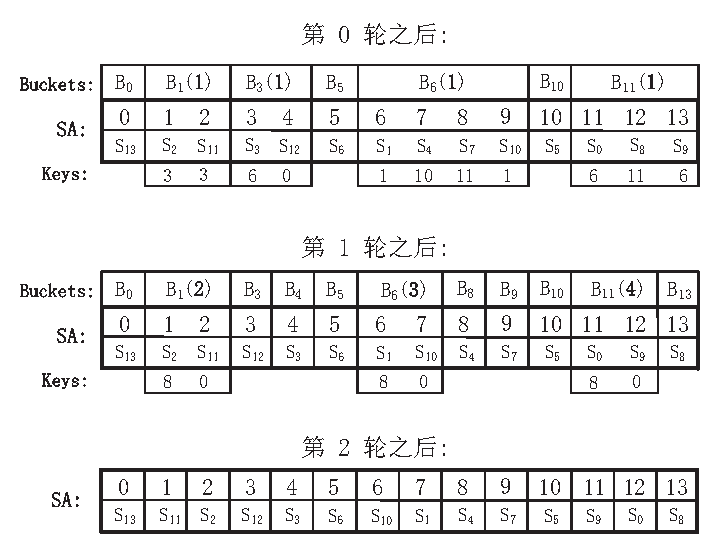
\includegraphics[height=8.5cm ,width=12.5cm]{figures/3_SS/dsufsort}
\vspace*{8pt}
\caption{使用 \emph{dsufsort} 算法对字符串 $\emph{tobeornottobe}$ 的后
  缀进行排序。}
\label{fig:1}
\end{figure}

\textbf{例子.} 图 \ref{fig:1} 说明了使用 \emph{dsufsort} 算法对输入字符
串 $tobeornottobe$ 进行后缀排序的过程。 为了清晰起见, 我们将完整的后
缀 $S_i$ 放入SA中, 而非其起始位置 $i$。 每个桶的深度在其后的括号内显
示。 第0轮过后, 所有后缀都基于其首字符被排序。 由于桶 $B_0$,
$B_5$ 及 $B_{10}$ 都只包含一个后缀, 这三个桶已经完全有序了。

在第1轮中, 产生于第0轮的4个未被排序的桶 $B_1$, $B_3$,
$B_6$ 及 $B_{11}$ 将被依次处理。 将处理 $B_6$ 作为例子, 其余3个桶可以类
似方式处理。 对 $B_6$ 中任一后缀 $S_i$, 其键值可以通过桶的深度来计算:
$key(S_i) = B[i+D[6]]$。 所以, $B_6$ 中所包含后缀的键值分别为:
$key(S_1) = B[1+D[6]] = 1$, $key(S_4) = B[4+D[6]] = 10$,
$key(S_7) = B[7+D[6]] = 11$, $key(S_{10}) = B[10+D[6]] = 1$。 然后, 使用
普通的整数排序函数对这些键值进行排序: $key(S_1) = key(S_{10}) <
key(S_4) < key(S_7)$。  根据键值的大小顺序, $B_6$ 中后缀的 1-序 可以被确
定: $S_1 =_ 1 S_{10} \prec_1 S_4 \prec_1 S_7$。 由于 $S_1$ 和 $S_{10}$
具有同样的键值, 它们将共同构成一个新的未排序桶 $B_6$。 注意, 相比于原先
的(即当前正在被处理的) $B_6$(由 $B_6^{\;old}$ 表示), 新产生
的 $B_6$(由 $B_6^{\;new}$ 表示) 具有相同的桶序号 (这意味
着 $S_1$ 和 $S_{10}$ 所在的桶不变), 但不同的大小和深度。 $B_6^{\;new}$
的深度为 $D[6]^{\;new} = D[6]^{\;old} + D[1] = 3$, 这是因
为 $B_1$是 $B_6^{\;new}$ 的锚桶且 $D[1] = 2$。 另一方面, $S_4$ 和 $S_7$
都具有唯一的键值, 它们将分别构成完全有序的桶 $B_8$ 和 $B_9$, 且仅需要更
新它们所在的桶号: $B[4] = 8$, $B[7] = 9$。 第1轮过后, 将剩余3个未排序的
桶: $B_1^{\;new}$, $B_6^{\;new}$, $B_{11}^{\;new}$。

在第2轮中, $B_1^{\;new}$, $B_6^{\;new}$ 及 $B_{11}^{\;new}$ 将会依次被
处理。 通过使用 $D[1] = 2$, $D[6] = 3$ 及 $D[11] = 4$ 来分别计算后缀的
键值并对其进行排序, 所有3个桶将会在本轮中被完全排序, 算法也随即结束。

为了说明 \emph{dsufsort} 相比于 \emph{qsufsort} 的优势, 考察在第1轮中
对 $B_{11}^{\;old}$ 的处理过程。 由于 $B_{11}^{\;old}$ 中所包含后缀的键
值分别为: $key(S_0)=6$, $key(S_9)=6$, $key(S_8) = 11$, $S_8$ 将构成完全
有序的桶 $B_{13}$, 而 $S_0$ 和 $S_9$ 将构成未排序的
桶 $B_{11}^{\;new}$。 由于 $B_{11}^{\;new}$ 产生于 $B_{11}^{\;old}$, 且
其锚桶为 $B_6^{\;new}$, 因此 $B_{11}^{\;new}$ 的深度为
$D[11]^{\;new} = D[11]^{\;old} + D[6]^{\;new}$。 正如已经知道的,
$B_6^{\;new}$ 同样也产生于第1轮, 且其深度为 $D[6]^{\;new} =
3$, 所以 $D[11]^{\;new} = 1 + 3 = 4$。 因此 $B_{11}^{\;new}$ 的深度大
于2 (在 \emph{qsufsort} 的第1轮中, 所有桶的"深度"都为2)。 这样, 在第2轮
中, $B_{11}^{\;new}$ 中的后缀将至少基于其前 $4+2$ 个字
符 (而非\emph{qsufsort}算法所基于的前 $2+2$ 个字符) 被排序。 其后缀的键
值分别是: $key(S_0)=B[0+D[11] ^{\;new}]=
8$ 和 $key(S_9)=B[9+D[11]^{\;new}]= 13$, 这说明 $B_{11}$ 可以在第2轮中
被完全排序。 相比之下, 在 \emph{qsufsort} 算法中, $B_{11}^{\;old}$ 中后
缀的键值为 $key(S_0) = B[0+2] = 1$ 及 $key(S_9) = B[9+2] = 1$, 这意味
着 $B_{11}^{\;old}$ 无法在第2轮中被完全排序。 所以, \emph{dsufsort} 算法
仅需要3轮便可对所有的后缀完成排序, 而 \emph{qsufsort} 算法则需要4轮。

对于平均LCP较大的输入字符串, \emph{dsufsort}算法所具有的"深度叠加"的特
性将充分发挥, 使其可以更快地确定具有较长公共前缀后缀的次序。


\section{高效地实现}
\label{sec:3_Implementation}

本节中, 将讨论一些用于提高算法效率的实现技巧。

\subsection{输入变换}

在第0轮中, 所有后缀都将基于其首字符被排序。 实际上, 通过预先对输入字符串
进行变换, 可以使后缀根据前几个字符进行排序。 输入变换包括以下两个步骤:

1. 字符集压缩

给定$\Sigma$上的字符串 $T = t_0t_1...t_{n-1}\$$, 令实际出现于$T$ 中的字
符构成有序集 $C = \{c_0, c_1,\dots, c_{m-1}\}$, 其中 $c_i < c_j \iff i
< j$。 注意, 末尾的终结字符 '\$', 一定是 $c_0$。 然后, 对$T$中的每一个字
符 $t_i$, 将其替换为$t_i$ 在 $C$ 中的序数, 即: $t_i \mapsto j \iff t_i
= c_j$。 通过使用这种映射,
$T$ 中的每个字符将被映射为一个整数, 同时保持后缀之间的顺序不变。 通过字
符集压缩, $\Sigma$ 将被转化为较小的整数集: $\{0,1,\dots,m-1\}$。

2. 字符累加

通过对 $T$ 使用字符压缩, 可以得到一个大小为 $m$ 的整数集:
$\{0,1,\dots,m-1\}$。 令 $k$ 为最大的整数, 使得 $m^k-1$ 可以由一个典型的
机器整数类型表示(比如 int型)。 然后, 对 $T$ 的每个后缀, 将其前 $k$个字符
通过以下方式累加:

\begin{equation}\label{eq:ca1}
  T[i] = \sum_{j=1}^k t_{i+j-1} \cdot m^{k-j}  ~~(0 \leq i \leq n),
\end{equation}

\noindent 其中, 定义 $t_s = 0$, 对于所有 $s \geq n$。 在第0轮中,
$T[i]$将作为 $S_i$ 的键值, 这样, 排序将不仅仅基于后缀的首字符, 而是其
前 $k$个字符。 随后的排序过程将从深度为 $k$的桶开始, 而不是深度
为1的桶, 因此,所需要的排序轮数也会减少。 公式 (\ref{eq:ca1}) 可以由以下
线性时间算法替代:

\begin{equation}\label{eq:ca2}
 T[i]  = \left\{
  \begin{array}{lll}
    \sum_{j=1}^{k}(t_{j-1} \cdot m^{k-j})  &,  &  i = 0\\
    (T[i-1]~ mod~m^{k-1}) \cdot m + t_{i-1+k} &,  & 0 < i \leq n \\
    \end{array}\right.
\end{equation}

\noindent
其中, 对于 $s \geq n$ 令 $t_s = 0$。 乘法和取模操作可由更快的"按位与"和
移位操作实现。

注意, 由于在对 $T$ 进行字符累加后, 其字符集将变得不再连续, 所以需要再次
对累加后的$T$使用字符集压缩技术。

\subsection{初始桶排序}

算法的第0轮 (初始化) 将独立于算法的其余部分, 它不需要使用和后续过程相同
的排序方法。 由于这一轮将处理所有的后缀, 通过使用一个线性时间复杂度的桶
排序算法来取代基于比较的$O(nlogn)$时间算法, 可以使算法性能得到很大提升。

一种十分有效的方式是结合桶排序算法和以上介绍的输入变换技术。 给定字符
串 $T = t_0t_1 \dots t_{n-1}\$$, 假设对 $T$ 进行输入变换之后, 新的字符
集为 $I = \{0,1,\dots,m-1\}$。 对 $I$ 中每一个整数 $i$, 它在$T$ 中的出现
频率记录在一个长为 $m$ 的数组 $F$ 中。 具体地讲,如果整数 $i$ 在 $T$中出
现了 $j$ 次, 则有 $F[i] = j$, 基于此, 一定有 $\sum_{i=0}^{m-1} F[i] =
n + 1$。 综上, \emph{dsufsort} 算法的第0轮包括以下4个步骤:

\begin{enumerate}
\item 初始化 $F$: $\forall i \in I$, 令 $F[i] = 0$。
\item 正向扫描 $T$, 计算其中每个字符的出现频率: 对 $i =
  0,\dots,n$, 将 $F[T[i]]$ 加1。
\item 正向遍历 $F$, 相加相邻元素: 对 $i = 1, \dots, m-1$, 令 $F[i] =
  F[i] + F[i-1]$。
\item 反向扫描 $T$, 将其每个后缀放入适当的桶内: 对 $i = n, n-1,\dots,
  0$, 将 $F[T[i]]$ 减1, 同时令 $SA[F[T[i]]] = i$。
\end{enumerate}

第0轮过后, SA将被划分为$m$个桶 (完全有序的或未排序的), 且未排序的桶中所
包含的后缀, 其前$k$个字符都相同。 实际上, "桶排序"中的"桶"的概念特指由定
义5中所定义的深度为$k$的桶。

\subsection{选择整数排序算法}

前面提到过, \emph{qsufsort} 算法和 \emph{dsufsort} 算法都需要一个整数排
序子程序来对键值进行排序, 因此, 该整数排序子程序对算法整体的性能具有重
要影响。 本章中所使用的子程序被称为 \emph{split-end
  partitioning}, 由Bentley和Mcllroy\cite{Bentley1993} 提出。 它是著名的
快速排序算法\cite{Hoare1962}的一种变体, 使用了三元分割策略。

经典的快速排序算法使用二元分割策略, 递归地将待排序数组分为两部分, 其中
一部分的元素小于枢轴元素, 令一部分的元素大于枢轴。 接着, 这两部分将被递
归地处理, 直到整个数组有序。 快速排序算法将相等于枢轴的元素放入其中一个
数组部分或同时放入两个部分, 取决于具体实现。 然而, 使用三元分割
的 \emph{split-end partitioning} 算法将数组划分为3个部分: 一部分元素小
于枢轴, 一部分元素大于枢轴, 另一部分元素等于枢轴。 大于或小于枢轴元素的
部分将被递归地排序, 而等于枢轴的部分则保持不变, 因为其中元素已经处于正
确的位置。

对 \emph{split-end partitioning} 算法的实现将直接基于Bentley和Mcllroy
\cite{Bentley1993} 中的Program 7, 只有一点例外: 为了快速处理较小的桶,
将使用一种非递归的选择排序方法来处理后缀数量小于7的桶。

\section{实验结果}
\label{sec:3_Experiment}

本节将比较 \emph{dsufsort} 算法和其它三个比较知名的算法
即 \emph{qsufsort} \cite{Larsson2007},
\emph{DC32}\cite{Burkhardt2003} 算法, 和 \emph{KS} 算法\cite{Karkkainen2006}。 其中
\emph{dsufsort} 算法是 \emph{qsufsort} 算法的改进。 \emph{DC32} 算法是
将 difference-cover设置为模32的 \emph{difference-cover} 算法。
\emph{KS} 是最快的具有线性时间复杂度的后缀排序算法之一。 通过使用现实世
界中的数据和人工产生的(具有较大平均LCP的)数据来评估测试算法的性能。

实验在一台笔记本电脑是进行, 软硬件配置如下: Intel Core i7-2630QM
2.00GHz CPU, 8GB RAM, 500GB 磁盘。 操作系统为 Ubuntu 14.04-64bit。  所有
算法由 C/C++ 实现, 由 \emph{gcc} 4.8.2 编译 (-O3)。 为了确保算法实现的正
确性, 所有测试算法的排序结果都由Burkhardt \cite{Burkhardt2003} 提供的检测程
序 \emph{suffix array checker} 检验。

\begin{table}[!htbp]
\topcaption{测试数据集特征。}
\begin{tabular}{ccrrrr} \hline Files & Description & Size(bytes) &
  $|\Sigma|$ & Average LCP & Max LCP \\ \hline
  Proteins & Protein sequence & 66,804,271 & 20 & 33.46 & 6380\\
  XML & XML files & 294,724,056 & 97 & 44.91 & 1084 \\
  Pitches & MIDI pitch values & 55,832,855 & 133 & 262.00 & 25178\\
  Sources & C/Java source code & 210,866,607 & 230 & 371.80 & 307871\\
  DNA & DNA sequence & 403,927,746 & 4 & 2420.73 & 1378596\\
  English & English text & 2,210,395,553 & 235 &6675.35 & 987770\\
  \hline
  \end{tabular}
  \label{tab:data}
\end{table}

实验所使用的现实世界数据来源于 \emph{Pizza Chili Corpus}
(http://pizzachil.dcc.uchile.cl) 语料库, 其中包含6中类型的数据: 源代
码 (source code), 音符 (pitch values), 蛋白质序列 (protein sequence),
DNA 序列(DNA sequence), 英文文本 (English text), 和 XML文本 (XML
files)。 数据集的各种属性信息在表 \ref{tab:data}中显示, 包括数据集大
小 (size), 每个文件(字符串)的平均/最大LCP。 字符串的平均/最大LCP指的是为
该字符串所构建的后缀数组中, 任意相邻后缀的平均/最大LCP。 字符串的最
大LCP等价于字符串中最长重复子串的长度。 这些特性参数能够较好的反映数据的
重复程度。

\begin{table}[!htbp]
  \centering
  \renewcommand{\arraystretch}{1.5}
  \topcaption{测试算法的平均排序时间(以秒位单位)。}
  \begin{tabular}{crrrrr}
    \hline
    Files & Size   & dsufsort  & qsufsort & DC32  & KS\\
    \hline
    Proteins   & 100MB  & 25.34 &\textbf{24.11}    & 35.43 & 98.91\\
    XML        & 100MB  & 27.59 &\textbf{26.75}    & 49.54 & 67.39 \\
    Pitches    & 50MB   &\textbf{9.27 } & 10.52    & 12.42 & 32.83 \\
    Sources    & 100MB  &\textbf{23.81} & 25.64    & 33.03 & 83.03 \\
    DNA        & 100MB  &\textbf{26.02} & 28.90    & 38.15 & 85.44 \\
    English    & 100MB  &\textbf{41.72} & 44.35    & 48.20 & 97.12 \\
    \hline
    aaa\dots    & 100MB  &\textbf{9.14}  & 10.65 & 73.32 & 11.87\\
    abab\dots   & 100MB  &\textbf{8.82}  & 11.55 & 30.23 & 9.56\\
    rand-5-rep  & 100MB   &\textbf{10.36} & 16.32 & 35.60 & 12.77 \\
    rand-10-rep & 100MB   &\textbf{16.73} & 24.28 & 33.57 & 17.53 \\
    rand-20-rep & 100MB   & 23.11 & 39.03 & 35.92  & \textbf{22.85} \\
    \hline
  \end{tabular}
  \label{tab:time}
\end{table}

表 \ref{tab:time} 显示了每个测试算法基于10次独立运行的平均运行时间, 其
中最好的结果将加粗显示。 我们同样使用了人工产生的重复数据来测试算法的鲁
棒性。 前两个人工产生的文件分别由单个字符 'a' 和 字符块 'ab' 组成, 随后
的三个具有 \emph{rand-k-rep} 形式的文件, 是由长度为 $k$ 的随机字符串重
复出现, 直到构成100MB的数据。

从实验结果可得, 对于真实数据, \emph{dsufsort} 和 \emph{qsufsort} 算法表
现地最好, 其中对于大多数真实数据, \emph{dsufsort} 要优
于 \emph{qsufsort} 算法。 仅仅对于蛋白质和XML这两种平均LCP极低的数据,
\emph{dsufsort} 稍逊于 \emph{qsufsort}。 主要原因
是, 相比 \emph{qsufsort}, \emph{dsufsort} 算法在运行过程中需要实时更
新 $D$ 数组, 这需要额外的时间开销。 而对于平均LCP极低的数据, 由深度累加
技术所带来的时间上的收益, 将不足以抵消更新 $D$ 数组的开销。

对于平均LCP相对较高的人工数据, \emph{dsufsort} 算法可以极大地节省运行时
间。 表 \ref{tab:time} 中的结果显示, \emph{dsufsort} 对于大部分人工数据
都优于其它算法, 除了在 \emph{rand-20-rep} 数据上稍逊于线性时间算
法 \emph{KS}。 这是由于, 线性时间算法的性能较为稳定, 受测试数据特性的影
响较小。 然而, \emph{KS} 算法对于普通真实数据并不十分高效, 这限制了其在
实际环境中的应用。

综上所述, 对于绝大多数测试数据, \emph{dsufsort} 算法的性能都是最优
的。 仅仅对于平均LCP极低或极高的数据, \emph{dsufsort} 稍逊
于 \emph{qsufsort} 和 \emph{KS} 算法。

\section{本章小节}
\label{sec:3_Conclusion}

本章提出了一种基于\emph{qsufsort}算法的高效的后缀排序算
法 \emph{dsufsort}。 不同于 \emph{qsufsort} 算法在每轮中都依据固定数量的
前缀字符来对后缀进行排序, \emph{dsufsort} 会维持每个未排序桶的深度, 并
基于桶深来对其中后缀进行排序, 其深度累加效应使得 \emph{dsufsort} 相比
于 \emph{qsufsort} 算法更加高效, 尤其对于平均LCP较大的数据。

未来将关注于两个问题: 首先, 在当前的实现中, 未排序的桶将按照从左到右的
顺序依次处理, 然而, 对桶的处理顺序会对算法的性能造成一定影响, 所以我们
将致力于寻求最优的桶处理顺序。 其次, 用来记录桶深的 $D$ 数组可能会非常稀
疏, 这会增加空间开销, 所以研究稀疏数组压缩技术也非常重要。


  % Searching for the Multiple Longest Common Subsequences (MLCS) of
  % multiple sequences is an important NP-hard problem which has been
  % widely used in many areas, such as biomedicine and
  % bioinformatics. The most effective approaches for this problem until
  % now is based on dominant point graph. However, the time and space
  % efficiency of the leading dominant point graph based approaches is
  % still unsatisfactory: the dominated point Directed Acyclic Graphs
  % (DAG) constructed by these algorithms consume a huge amount of
  % memory and time during processing, which limits the applications of
  % these algorithms to large-scale and long sequences. Therefore, it is
  % very necessary and urgent to design time and space efficient methods
  % for MLCS problems with large-scale and long sequences.  In this
  % paper, we set up a new time and space efficient graph model called
  % the Leveled-DAG for MLCS problems. During processing, the
  % Leveled-DAG model can timely eliminate all nodes in the DAG that can
  % not contribute to the construction of MLCS. At any moment, only the
  % current level and a very small part of previously generated nodes in
  % the DAG need to be kept in the memory.  Also, the final graph
  % contains only one node in which all of the MLCS are saved, thus, no
  % further operations for searching the MLCS are needed. The
  % experiments are conducted on real biological sequences with
  % different numbers and lengths, respectively, and the proposed
  % algorithm is compared with three state-of-the-art algorithms. The
  % experimental results show that the time and memory needed for the
  % proposed approach are much smaller than those for the compared
  % algorithms especially on large-scale and long sequences.




\chapter{求解最长公共子序列(MLCS)问题的层次化图模型}

\section{引言}
\label{sec:introduction}

度量生物序列间的相似性是生物信息学中的一类基本问题,它们在癌症检
测\cite{Aravanis2017,Chattopadhyay2016,Munday2017},探寻物种的共同起
源 \cite{Zvelebil2007,Perry2015,Donnell2015} 等许多方面具有广泛的应用。
度量序列间相似性最重要手段之一是寻找序列间的最长公共子序列 (Longest
Common Subsequence,简称为LCS), 这已被证实是一类NP难问
题\cite{Maier1978}。根据目标序列的个数,该问题可以被分为两类:(1)寻找两
个序列的最长公共子序列被称为最长公共子序列(LCS)问题;(2) 寻找超过两个序
列的最长公共子序列被称为多最长公共子序列(MLCS)问题。

传统上, 研究工作主要集中于第一类问题。然而近些年来,越来越多的来自生物
信息学及其他领域的应用要求寻找超过两个序列的最长公共子序列(MLCS)。例如,
多序列比对(Multiple Sequence Alignment) 是MLCS问题在生物信息学中最主要
的应用之一 \cite{Katoh2016,Zou2015,Mirarab2015,Bawono2017,Chatzou2015},
该技术能够重排多个DNA,RNA,或蛋白质序列,找出序列间具有相似性的片段,
以此来识别序列间功能性的,结构性的,或进化性的联系。 MLCS算法同样可以应
用到许多其他种类的序列中,比如在自然语言处理中计算字符串之间的编辑距离,
以及应用到许多金融类数据中。目前,针对这些应用的现有算法大多基于支配点
图模型--该类算法将基于目标序列构建支配点有向无环图(DAG),从而将寻找序
列MLCS的问题转化为寻找有向无环图中最长路径的问题。但是由于这类算法构
造DAG的时间/空间开销过大,使其无法应用于多序列或长序列的情形。

本章中,我们提出了一种时空高效的有向无环图模型,被称为“层次化有向无环图”(简称
为Leveled-DAG),同时设计了相应的构建算法。类似于现有(基于支配点的)算法中的有向无
环图的构造方式,Leveled-DAG模型将被逐层地构造,然而,区别于现有算法在构造有向无环
图时需要产生大量节点并将其全部保存在内存中, Leveled-DAG模型会实时地删除那些过时的
节点, 这些节点不会对构造MLCS再产生影响的。 在任意时刻,Leveled-DAG只需保存新产生
的一层节点及部分以前产生的节点,因此,Leveled-DAG的规模比现有算法构造的有向图无环
图小很多,这会极大的减少空间开销。此外,随着构建过程的进行,Leveled-DAG的规模将越
来越小,最终将只包含一个节点(终止节点),而目标序列的MLCS都存储在该节点中从而直接
可得,无序任何额外操作来寻找MLCS,这将节省算法的运行时间, 提高算法效率。 实验结果
证实,Leveled-DAG模型在时间和空间两方面均非常高效,尤其对于大规模或长序列
集,Leveled-DAG模型明显优于现有方法。

本章组织如下: 节介绍了背景知识及相关工作;节详细的介绍了Leveled-DAG模型及其构建
算法;节进行了仿真实验和结果分析;节总结了本章内容。

\section{相关概念}
\label{sec:MM}

首先, 令 $\Sigma$ 表示序列的\emph{字符集}, 即序列中所出现符号的有限集
合。 例如, DNA序列的字符集是: $\Sigma=\{A, C, G, T\}$。

\textbf{定义 1.} 令 $\Sigma$ 表示序列的字符集,令 $s=c_1c_2...c_n$ 表示
长为 $n$的一个\emph{序列},其中每个字符 $c_i\in\Sigma$,
$i=1,2,\cdots,n$。 序列 $s$ 中的第 $i$ 个字符表示为 $s[i]=c_i$。 如果一
个序列 $s'$ 是由删除 $s$ 中零个或多个(不一定连续)字符而得到的,
即 $s'=c_{i_1}c_{i_2}...c_{i_k}$ 且满足
$1 \leq i_1<i_2<\cdots<i_k \leq n$, 则序列 $s'$ 被称为序列 $s$ 的一个长
为 $k$ 的\emph{子序列}。

\textbf{定义 2.} 给定字符集 $\Sigma$ 上的 $d$ 个序列 $s_1, s_2, ...,
s_d$, 如果一个序列 $s'=c_{i_1}c_{i_2}...c_{i_k}$ 满足: (1) 它是 $d$ 个
序列中每一个序列的子序列。 (2) 它是 $d$ 个序列最长的子序列。 则 $s'$ 被
称为这 $d$ 个序列的\emph{最长公共子序列}(简称为LCS)。

通常, 多个序列的最长公共子序列并不唯一。 例如,给定三个DNA序列 $ACTAGTGC$,
$TGCTAGCA$ 和 $CATGCGAT$, 它们有两个长为4的最长公共子序列,分别
是 $CAGC$ 和 $CTGC$。 所谓的多最长公共子序列(MLCS)问题, 就是要找出三个或多个目标序
列的所有最长公共子序列。

针对MLCS问题,在过去几十年中,许多算法已被提出。根据这些算法所基于的模型,它们可
以被分为两大类:基于动态规划的算法和基于支配点模型的算法。下面将简要介绍这两类方
法。

\subsection{基于动态规划的算法}
\label {sec:Dynamic Programming}

求解MLCS问题的经典方法基于动态规划 \cite{Smith1981}, \cite{Sankoff1972}。 给定$d$
个序列 $s_1,\, s_2,\,...,\, s_d$, 其长度分别为 $n_1,\, n_2,\, ...,\, n_d$, 基于动
态规划的算法将递归的构造一个具有 $n_1 \times n_2 \times ... \times n_d$ 个元素
的“得分矩阵” $T$, 其中元素 $T[i_1,\, i_2,\, ...,\, i_d]$ 记录了前缀序
列 $s_1[1...i_1]$, $s_2[1...i_2]$, ..., $s_d[1...i_d]$ 的最长公共子序列的长
度。 元素 $T[i_1,\, i_2,\, ...,\, i_d]$ 可由以下公式递归计算:

\begin{equation}
  T[i_1,\, i_2,\, ...,\, i_d] =
  \begin{cases}
    0 & \text{if $\exists j(1 \leq j \leq d), i_j = 0$}\\
    T[i_1-1,\, ...,\, i_d-1] + 1  & \text{if $s_1[i_1] = s_2[i_2] =
      ... = s_d[i_d]$}\\
    max(\bar{T}) & \text{otherwise}
  \end{cases}
\end{equation}

其中
$\bar{T} = \{T[i_1-1,\, i_2,\, ...,\, i_d],\, T[i_1,\, i_2-1,\, ...,\, i_d],\,
...,\, T[i_1,\, i_2,\, ...,\, i_d-1]\}$。 一旦得分矩阵 $T$ 构建完成, 目标序列的最
长公共子序列可由 $T$ 的最后一个元素 $T[n_1,\, n_2,\, ...,\, n_d]$ 向其第一个元
素 $T[0,\, 0,\, ...,\, 0]$ 进行反向回溯而得到。 图 \ref{fig:DM} A 显示了两个序
列 $s_1 = ACTAGCTA$ 和 $s_2 = TCAGGTAT$ 的得分矩阵 $T$。 如图\ref{fig:DM} (B) 所
示, 这两个序列的最长公共子序 (分别是 $TAGTA$ 和 $CAGTA$), 可由元素 $T[8,\, 8]$
向元素 $T[0,\, 0]$ 进行回溯而得到。

\begin{figure}[!h]
  \centering
  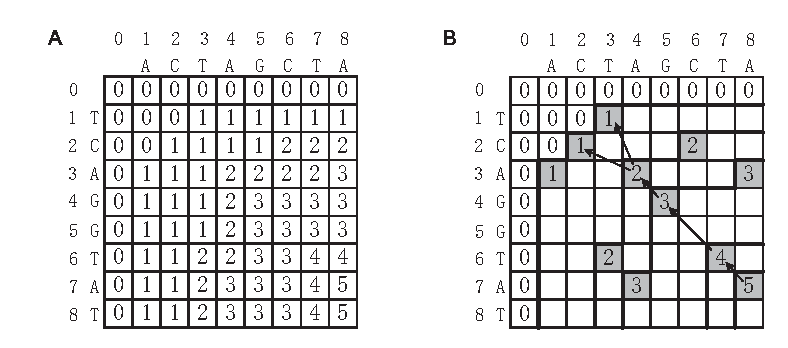
\includegraphics[height=2in, width=4.5in]{figures/4_MLCS/DM}
  \vspace{1em}
  \caption{(A) 两个DNA序列 ACTAGCTA 和 TCAGGTAT 的得分矩阵。 (B) 通过得分矩阵构建
    最长公共子序列,其中的阴影元素对应于支配点。}
\label{fig:DM}
\end{figure}

很明显,对于具有相同长度 $n$ 的 $d$ 个序列, 使用基于动态规划的算法求解
其MLCS的时间和空间复杂度均为 $O(n^d)$ \cite{Hsu1984}。 已经有许多算法被
提出用于改进基于动态规划方法的效
率 \cite{Hirschberg1977,Apostolico1992,Masek1980,Rick1994}。 然而, 随着
$d$ 和 $n$ 的增加, 所有这些方法的效率仍然无法满足实际需求。

\subsection{基于支配点的算法}
\label{sec:Dominant Point}

为了减少基于动态规划方法的时空复杂度,许多新方法已被提出,基于支配点图模型的算法
是其中最有效的方法之一。在介绍该方法前首先给出一些基本定义。

\textbf{定义 3.} 给定 $\Sigma$ 上的 $d$ 个序列 $s_1,\, s_2,\, ...,\,
s_d$, 向量 $p = (p_1,\, p_2,\, ...,\, p_d)$ 被称为这 $d$ 个序列的一
个\emph{匹配点}, 如果其满足 $s_1[p_1] = s_2[p_2] = ... = s_d[p_d] =
\delta$, 即 $\delta$ 是位于序列 $s_i$ 第 $p_i$ ($i=1,2,\cdots,d$) 个位
置的公共字符。 匹配点 $p$ 所对应的公共字符 $\delta$ 表示为 $C(p)$。

\textbf{定义 4.} 给定 $d$ 个序列的两个匹配点 $p = (p_1,\, p_2,\,
...,\, p_d)$ 和 $q = (q_1,\, q_2,\, ...,\, q_d)$, 我们称: (1) $p =
q$当且仅当 $p_i = q_i$ ($1 \leq i \leq d$); (2) $p$
\emph{支配 }$q$ 或 $q$ 被 $p$ 支配 (表示为 $p \preceq q$), 如果对每一
个 $i$ ($1 \leq i \leq d$) 都有 $p_i \leq q_i$, 并且存在 $j$
($1 \leq j \leq d$) 使得 $p_j<q_j$; (3) $p$ \emph{强支配}
$q$ 或 $q$ 被 $p$ 强支配 (表示为 $p \prec q$), 如果对每一个 $i$ ($1
\leq i \leq d$) 都有 $p_i < q_i$; (4) $q$是 $p$ 的一
个\emph{后继}或 $p$ 是 $q$ 的\emph{前驱}, 如果 $p \prec q$ 并且不存在匹
配点 $r$ 使得 $p \prec r \prec q$ 且 $C(q) = C(r)$。

注意, 一个匹配点最多有 $|\Sigma|$ 个后继, 其中每个后继对应于 $\Sigma$ 中的一个字
符。

\textbf{定义 5.} 匹配点 $p = (p_1,\, p_2,\, ...,\, p_d)$ 所在的\emph{层
  次}被定义为 $L(p) = T[p_1,\, p_2,\, ...,\, p_d]$, 其中 $T$ 是由公
式 (1) 计算得到的得分矩阵。 匹配点 $p$ 被称为一个 $k$-支配点, 当且仅当:
(1) $L(p) = k$。 (2) 不存在其他匹
配点 $q$ 使得 $L(q) = k$ 且 $q \preceq p$。 所有 $k$-支配点构成了集合 $D^k$。\\

基于支配点模型的方法的动机在于减少动态规划方法的时空复杂度。 其核心思想基于这样的
事实,即只有支配点才能够影响MLCS的构建(如图\ref{fig:DM} B 所示, 阴影元素对应于
支配点)。由于支配点的数量远小于矩阵 $T$ 中的所有元素的数量,而基于支配点模型的方
法将只需计算支配点而非整个矩阵的元素,因此相比动态规划方法极大地降低了时空复杂
度。

基于支配点模型的算法的搜索空间可以被组织为一个有向无环图(DAG): 图中的每一个节点代
表一个匹配点,边 $\langle p,\, q \rangle$ 代表 $q$ 是 $p$ 的一个后继,即 $p
\prec q$ 且 $L(q) = L(p) + 1$。 最初, 图中仅包含一个没有任何入边的源节点 $(0,\,
0,\, ...,\, 0)$ 以及一个没有任何出边的终止节点 $(\infty,\, \infty,\, ...,\,
\infty)$。 接着, 有向无环图将按照如下方式被逐层构造: 首先, 令层次 $k =
0$, 且 $D^0 = \{(0,\, 0,\, ...,\, 0)\}$, 然后,
通过一个正向迭代的过程:$D^k \rightarrow D^{k+1}$, $(k+1)$-支配点集 $D^{k+1}$ 将
基于 $k$-支配点集 $D^k$ 而产生。 具体地, $D^k$ 中的每个节点将会通过产生其所
有 $|\Sigma|$ 个后继而被扩展, 接着通过一个被称为 $Minima$ 的剪枝操作找出所有那些
支配其它节点的支配点,只有这些支配点才被保留下来以构成 $D^{k+1}$。 一旦图中所包含
的所有节点均已被扩展, 整个有向无环图便构造完毕, 图中从源节点到终止节点的一条最长
路径对应于目标序列的一个最长公共子序列, 这样, MLCS 问题便转化为寻找图中从源节点到
终止节点的所有最长路径的问题。 下面将给出一个简单的例子来说明以上过程。

\textbf{例 1.} 基于支配点模型求解序列 $ACTAGCTA$ 和 $TCAGGTAT$ 的最长公共子序列,
如图 \ref{fig:DAG} 所示。

\begin{figure}[!h]
  \centering
  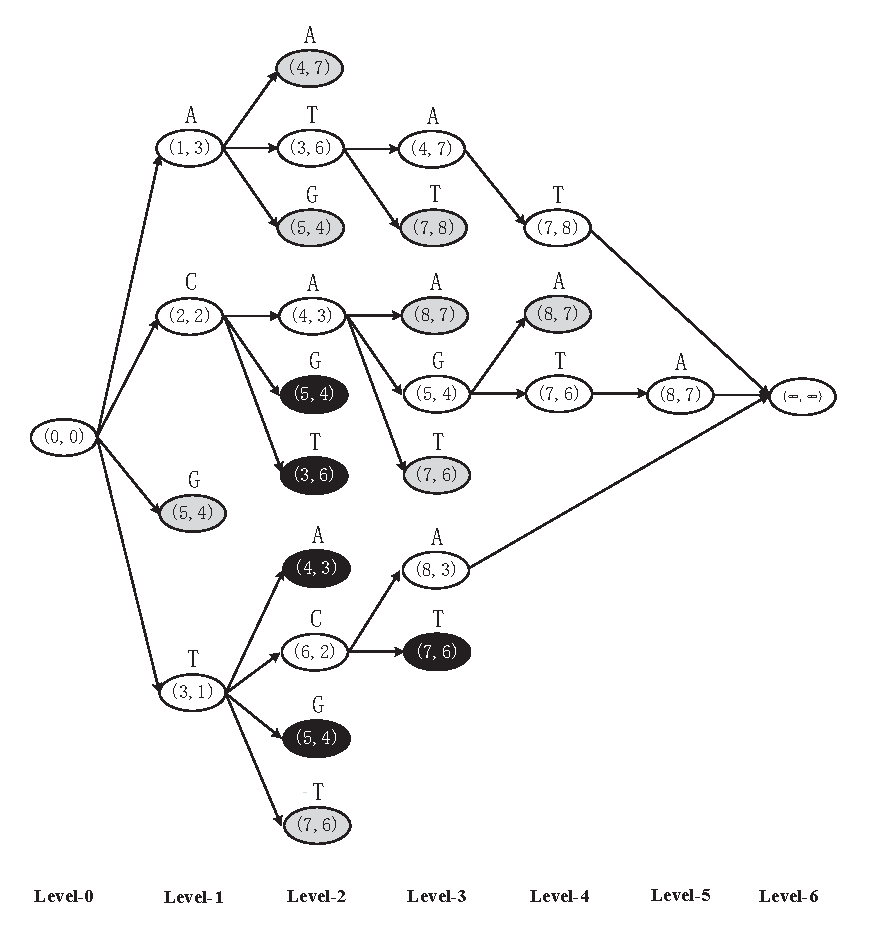
\includegraphics[height=3.8in, width=3.6in]{figures/4_MLCS/DAG}
  \vspace{1.5em}
  \caption{基于支配点模型所构造的序列 $ACTAGCTA$ 和 $TCAGGTAT$ 的有向无环图,图中
    黑色和灰色的节点将被 $Minima$ 剪枝操作删除。}
  \label{fig:DAG}
\end{figure}


\begin{itemize}
\item \textbf{步骤 0}. 产生源节点 $(0,0)$ 和终止节点 $(\infty, \infty)$。
\item \textbf{步骤 1.} 构造图的第一层节点。 对于字符 $A$, 其匹配点 $(1,3)$ 中的两
  个分量分别是 $A$ 在两个输入序列中第一次出现的位置。 这样, 节点 $A(1,3)$ 便是源
  节点在第一层中对应于字符 $A$ 的后继。 类似地, 节点 $C(2,2)$,
  $G(5,4)$ 和 $T(3,1)$ 是源节点分别对应于字符 $C$, $G$ 和 $T$ 的后继。 在第一层的
  这4个节点当中, 通过 \emph{Minima} 剪枝操作找出并删除被支配
  点 $G(5,4)$, 如图 \ref{fig:DAG} 中灰色节点所示。 剩下的3个支配节点构成了图的第
  一层 $D^1=\{A(1,3),C(2,2),T(3,1)\}$。
  
\item \textbf{步骤 2}. 构造图的第二层节点。 对于 $D^1$ 中的每一个节
  点, 比如 $A(1,3)$, 由于匹配点 $(4,7)$ 的分量是继匹配点 $(1,3)$ 之后字符 $A$ 在
  两个序列中第一次出现的位置。 这样, 节点 $A(4,7)$ 便是节点 $A(1, 3)$ 在第二层中
  对应于字符 $A$ 的后继。 类似地, 节点 $T(3,6)$ 和 $G(5,4)$ 是节点 $A(1, 3)$ 在第
  二层中分别对应于字符 $T$ 和 $G$ 的后继。 以此类推, 第一层中的节点 $C(2,2)$ 可以
  产生3个第二层中的后继节点: $A(4,3)$, $G(5,3)$ 和 $T(3,6)$,第一层中的节
  点 $T(3,1)$ 可以产生4个第二层中的后继节点: $A(4,3)$, $C(6,2)$,
  $G(5,4)$ 和 $T(7,6)$。 注意, 有些节点会被重复产生。 在新产生的第二层的10个节点
  中, 通过剪枝操作 \emph{Minima} 找到并删除重复节点 $A(4,3)$, $G(5,4)$ (会被删除
  两次) 和 $T(3,6)$, 如图第二层中的黑色节点所示。 同样, 通过 \emph{Minima} 操作
  找到并删除被支配节点 $(4, 7)$, $(5, 4)$ 和 $(7, 6)$ 如图第二层中的灰色节点所
  示。 剩余的支配点构成了图的第二层 $D^2=\{T(3, 6),\; A(4, 3),\;$ $C(6,2)\}$。 注
  意, 如果一个节点没有任何后继,那么令终止节点为其唯一后继。
\item \textbf{步骤 3}. 逐层重复以上步骤,直到有向无环图构造完毕,即图中所有节
  点(除了终止节点)均已被扩展。
  
\end{itemize}

从以上例子可以看出,基于支配点模型的方法有以下两个缺陷:
\begin{enumerate}
\item 每层中会产生大量重复的,被支配的冗余节点,它们将消耗大量的存储空间。
\item 找出并删除冗余节点的剪枝操作需要对大量的 $d$ 维向量进行逐对比较,每次比较又
  需要 $d$ 次整数比较,当 $d$ 较大时,对每一层进行剪枝操作将会变得极其耗时。
\end{enumerate}

Hunt \cite{Hunt1977} 首次提出了针对两个序列的基于支配点的算法,其时间复
杂度为 $O((r+n)logn)$, 其中 $r$ 是支配点图中节点的数量, $n$ 是两个目标
序列的长度。 此后,为了进一步提高算法效率, 各种基于支配点模型的变体算法
被相继提出。Korkin \cite{Korkin2001} 首次提出了并行MLCS求解算法,其时间
复杂度为 $O(|\Sigma||D|)$, 其中 $|D|$ 是支配点图中的节点数量。 Chen
\cite{Chen2006} 提出了一种针对DNA序列的高效算法 -- FAST-LCS, 它采用了一
种被称为后继表的新型数据结构,用来在常量时间内产生一个节点的所有后继,
同时使用了剪枝操作用来删除每一层中的非支配节点。 Wang \cite{Wang2011}
提出了 Quick-DPAR 算法用以改进 FAST-MLCS 算法, 它使用了“分而治之”的策
略来删除非支配点从而使其非常易于并行化, 作者称相比于串行版本的算法,其
并行化算法获得了近似于线性的加速比。Li \cite{Li2012} 和 Yang
\cite{Yang2010} 分别设计了在GPU上针对LCS问题的并行算法和在云平台上针
对MLCS问题的并行化算法。 遗憾的是, 由于过大的同步开销,Yang
\cite{Yang2010} 所提所提算法并不适用于包含很多序列的MLCS问题。 最近,
Li \cite{Li2016_ICDE} 和 Li \cite{Li2016_SIGKDD} 分别提出了两种基于支配
点模型的算法: PTop-MLCS 和 RLP-MLCS, 它们都使用了被称为“无冗余公共子序
列图”(简称为NCSG)的新的图模型, 该图模型在构建过程中能够极大地减少冗余
节点的产生, 同时算法采用了正反向拓扑排序来寻找图中的最长路径。作者称两
种算法的时空复杂度均线性于图中所包含的节点数量。

在实际当中,对于大序列集,传统算法需要花费大量的时间和空间来求解其最优
解(即完整的最长公共子序列集),为解决此问题,一系列近似算法被相继提出。
近似算法首先能够在极短的时间内找出一些次优解 (即非最长公共子序列),然后
通过反复迭代,逐步提高解的质量,最终使其逼近于真实的最优解。Yang
\cite{Yang2013} 提出了基于支配点模型的近似算法--Pro-MLCS及其并行化版
本。 Pro-MLCS 能够以仅仅 $3\%$ 的总运行时间找到近似解, 然后通过反复迭代
来提高解的质量, 迭代时间越长, 解的质量就越好。最近, Yang
\cite{Yang2014} 提出了另外两种近似算法 SA-MLCS 和 SLA-MLCS。 SA-MLCS 使
用了一种称为 “iterative beam widening” 的搜索策略来减少迭代过程中的空
间消耗。 基于 SA-MLCS, 空间受限型算法 SLA-MLCS 被提出, 它可以确保算法的
内存开销不超过预先设定的值。


\section{一种新的图模型: Leveled-DAG 及其构建算法}
\label{sec:Algorithm}

本节中将介绍Leveled-DAG图模型及其相应的构建算法,在描述细节之前,首先介绍一些将要
用到的核心数据结构。

\subsection{核心数据结构}
\label{sec:data structures}

I. 后继表
\label{sec:successor table}

高效地产生每一个节点的后继,是构建Leveled-DAG的关键步骤。为此,需要为每一个输入序
列构造一个后继表 \cite{Chen2006}。 通过查询这些后继表,能够在常量时间内产生一个节
点的后继。 具体地,给定序列 $s=c_1c_2...c_n$, 其所对应的后继表(由 $ST$ 表示)是一
个拥有 $|\Sigma| \times (n+1)$ 个元素的二维数组, 其中第 $i$ 行第 $j$ 列的元
素(由$ST[i, j]$表示)按照如下方式计算:

$$ST[i,j]=min\{m\;|\;c_m=\sigma_i,\; m > j,\; 1 \leq i \leq
|\Sigma|,\; 0 \leq j \leq n\}$$

其中 $\sigma_i$ 是字符集 $\Sigma$ 中第 $i$ 个字符。 事实上, $ST[i,j]$ 记录了在序
列 $s$ 的第 $(j+1)$ 个位置之后,字符 $\sigma_i$ 第一次出现的位置。 例如,
DNA序列 $ACTAGCTA$ 和 $TCAGGTAT$ 的后继表分别在图 \ref{fig:ST} A 和 B中所示。 给
定 $d$ 个长为 $n$ 的序列, 其后继表可以在 $O(d|\Sigma|n)$ 时间内构建完成。

\begin{figure}[!h]
  \centering
  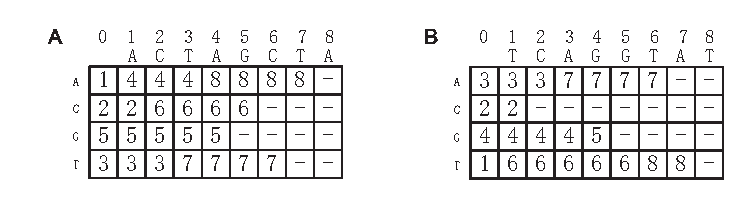
\includegraphics[height=1.2in, width=4.8in]{figures/4_MLCS/ST}
  \caption{(A) 序列 ACTAGCTA 的后继表。 (B) 序列 TCAGGTAT 的后继表。}
    \label{fig:ST}
  \end{figure}

  给定 $d$ 个序列, 通过查询后继表,一个节点的所有后继可以
  在 $O(|\Sigma|d)$ 时间内产生。 例如, 图 \ref{fig:DAG} 中节点 $C(2,
  2)$ 的后继可以通过查讯图\ref{fig:ST}中所示的后继表而得到:
  $(ST_1[1, 2],\;ST_2[1, 2]) = (4, 3)$,\,
  $(ST_1[2, 2],\;ST_2[2, 2]) = (6, -)$,\,
  $(ST_1[3, 2],\;ST_2[3, 2]) = (5, 4)$ and
  $(ST_1[4, 2],\;ST_2[4, 2]) = (3, 6)$, 分别对应于字符 $A$, $C$,
  $G$ 和$T$, 其中 $(6, -)$ 意味着 $(2, 2)$ 没有对应字符 $C$ 的后
  继。 事实上, 一个节点可以没有任何后继。\\

\noindent II. Leveled-DAG 中的节点结构
\label{sec:Node}

Leveled-DAG中的每个节点,比如 $t$, 包含了以下信息:

\begin{itemize}
\item 节点 $t$ 所对应的匹配点, 用来标识 $t$ 的唯一性。
\item $Suc(t)$: $t$ 所有后继的集合。
\item $P\_LCS(t)$: 从源节点到 $t$ 的所有最长路径所对应的序列集 (它们是最长公共子
  序列的前缀, 在下文中简称为“前缀序列”)。
\end{itemize}

节点 $t$ 的匹配点用于判断 $t$ 是否已经存在于图中。 后面将会看到, 当一个节点被删除
时,其所包含的前缀序列会由其后继节点继承并加以延长。 当Leveled-DAG构造完毕时,其
中仅剩的终止节点所包含的前缀序列就是要寻找的输入序列的最长公共子序列。\\

\noindent III. 全局数据结构
\label{sec:auxiliary}

\begin{itemize}
\item \emph{L\_DAG} : 用于保存图中的节点。
\item $Cur\_Level$ : 用于保存当前待扩展节点的队列。
\item $Next\_Level$ : 用于保存新产生节点的队列。
\end{itemize}



$L\_DAG$ 是一个映射表结构用于保存图中的节点, 一个节点可以通过其键值(即匹配点)进
行检索。每当一个新节点产生后,通过在 $L\_DAG$ 中检索其匹配点,可以判断该节点是否
已经存在于图中,如果不存在,便将其插入$L\_DAG$。 队列 $Cur\_Level$ 用于保存当前层
中待扩展节点, 而队列 $Next\_Level$ 用于保存新产生的下一层节点(即当前层中节点的后
继)。


\subsection{一种新的图模型: Leveled-DAG}
\label{sec:leveled DAG}

Leveled-DAG模型的核心特性是,它采用了一种被称为“产生-删除”的策略来控制图的规
模。 具体来说,每当新的一层节点产生之后,图中所有入度为零的节点(即没有任何边指向
其的节点)就会变得“过时”,因为它们不会再是后续产生节点的后继,其所包含的前缀序列
也因此不会再发生变化,所以可以安全地将其删除而不会对最终结果造成任何影响。通过及
时地删除过时节点可以极大地缩小图的规模并降低内存开销。 基于这种策
略,Leveled-DAG将会从源节点开始进行逐层构造,任意时刻,只有当前新产生层的节点以
及(以前产生的)入度不为零的节点会被保留下来。 一旦构建完成,唯一剩余的终止节点便已
包含了所有输入序列的最长公共子序列,无需任何图搜索操作,这将节省大量运行时间。 下
面将给出一个例子来说明Leveled-DAG模型的构造过程。

\begin{figure}[!h]
  \centering
  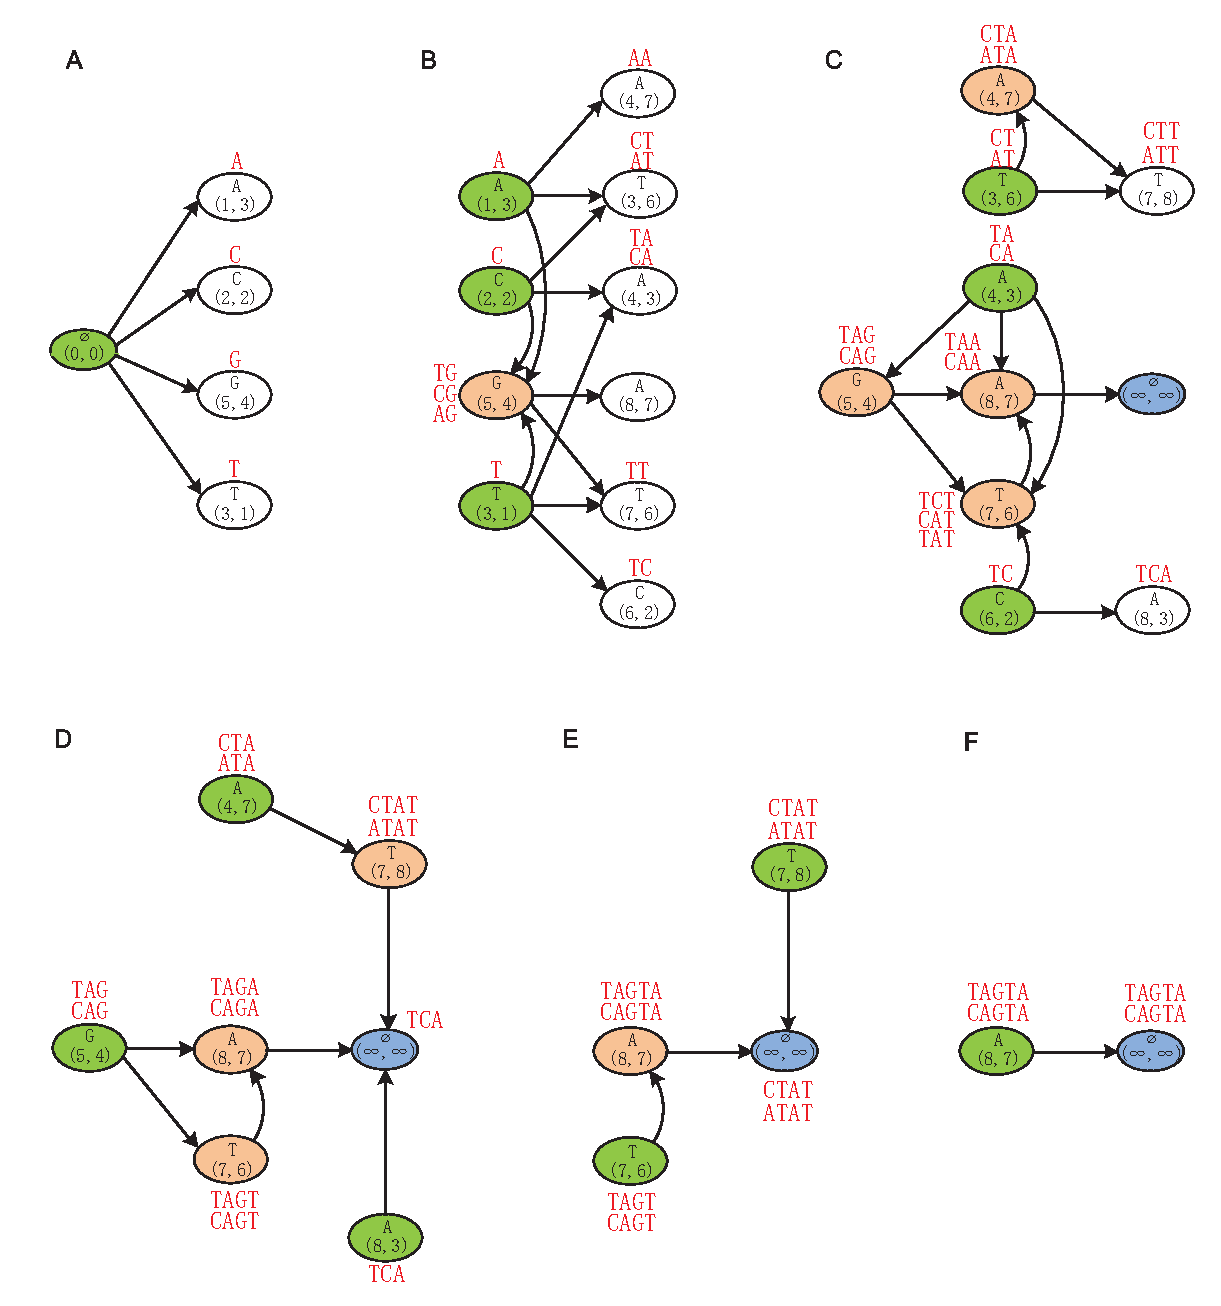
\includegraphics[height=4.5in,
  width=4.5in]{figures/4_MLCS/Level_DAG}
  \vspace{1.5em}
  \caption{序列 ACTAGCTA 和 TCAGGTAT 所对应的 Leveled-DAG。 匹配点及其
    对应字符在节点内部显示。 节点所对应的前缀序列,由其附近的红色字符串
    表示。 图中白色的节点是新产生的,且稍后将会被扩展。 绿色的节点已经
    过时,即将被删除。 之前产生的带有入边的红色节点,应当予以保留。}
  \label{fig:Leveled-DAG}
\end{figure}

\textbf{例 2.} 基于Leveled-DAG模型求解序列 $ACTAGCTA$ 和 $TCAGGTAT$ 的最长公共子
序列。 最初, Leveled-DAG只包含属于第0层的源节点 $(0, 0)$。 然后,通过查询
图\ref{fig:ST}中所示的后继表,产生源节点的4个后继: $A(1, 3)$, $C(2, 2)$, $G(5,
4)$和 $T(3, 1)$。 由于这4个后继属于第1层,它们的前缀序列分别是单个字符:$A$, $C$,
$G$ 和 $T$, 如图\ref{fig:Leveled-DAG} A 中对应节点上方的红色字符所示。 此时,由于
源节点入度为0,它已经过时,可以从图中安全删除。

然后,产生第1层节点的后继以构成第2层节点,这些后继是: $A(4, 7)$, $T(3, 6)$,
$A(4, 3)$, $A(8, 7)$, $T(7, 6)$ 和 $C(6, 2)$, 如图 \ref{fig:Leveled-DAG} B 所
示。 注意,如果一个后继已经存在于Leveled-DAG中 (比如 $G(5, 4)$), 它无需再重复产
生。 当第2层节点被产生之后, 由于节点 $A(1, 3)$, $C(2, 2)$ 和 $T(3, 1)$ 入度为0,
它们已经过时并将被删除, 此时, 其所包含的前缀序列需要被其后继节点继承并延
长。 例如, 已经过时的节点 $A(1, 3)$ 有3个后继: $A(4, 7)$, $T(3, 6)$ 和 $G(5, 4)$
(它没有对应于字符 $C$ 的后继)。 每一个后继都需要将其所对应的字符附加到 $A(1, 3)$
的前缀序列(即 $A$)之后, 然后将延长后的前缀序列保存为其自己的前缀序列。 具体地,
后继 $A(4, 7)$ 将 $A$ 附加到 $A$ 之后, 然后将 $AA$ 保存为自己的前缀序
列。 后继 $T(3, 6)$ 将 $T$ 附加到 $A$ 之后, 然后将 $AT$ 作为自己的前缀序列。 类似
地,后继 $G(5, 4)$ 将 $G$ 附加到 $A$ 之后, 将 $AG$ 作为自己的前缀序列。 注意, 由
于 $G(5, 4)$ 同时是这3个过时节点的后继, 它通过继承并延长这3个节点的前缀序列, 得
到了自己的3个前缀序列,分别是: $TG$, $CG$ 和 $AG$。 在移除过时节点之后,图中仅剩
余7个节点。

接下来, 如图 \ref{fig:Leveled-DAG} C 所示, 产生第2层所有节点的所有后继:$T(7,
8)$ 和 $A(8, 3)$ 构成图的第3层。 注意, 由于节点 $A(8, 7)$ 没有任何后继, 令终止节
点 $(\infty, \infty)$ 为其唯一后继。 在第3层构建完毕之后, 节点 $T(3, 6)$, $A(4,
3)$ 和 $C(6, 2)$ 已经过时。 在移除它们之前, 其所包含的前缀序列需要被其后继节点继
承并延长。 作为特例, 由于 $A(4, 7)$ 是过时节点 $T(3, 6)$ 的一个后继, $T(3, 6)$ 的
前缀序列 $CT$ 和 $AT$, 将由 $A(4, 7)$ 继承并加以延长(附加 $A$)。 由于延长后的前
缀序列 $CTA$ 和 $ATA$ 比 $A(4, 7)$ 原有的前缀序列 $AA$ 要长, $A(4, 7)$ 的前缀序
列将被相应地更新为 $CTA$ 和 $ATA$。 类似地, 节点 $G(5, 4)$ 和 $T(7, 6)$ 的前缀序
列同样通过继承并延长其过时前驱的前缀序列加以更新。

如图 \ref{fig:Leveled-DAG} D 所示, 需要扩展新产生的第3层中的节点 $T(7,
8)$ 和 $A(8, 3)$。 由于这两个节点均没有后继, 终止节点将被定义为这两个节点的唯一
后继。 由于没有新的节点产生, 此后将不再需要扩展任何节点。 从此刻起,算法只需要不
断地删除过时节点,并更新其相应后继节点的前缀序列。 当前, 节点 $A(4, 7)$, $G(5,
4)$ 和 $A(8, 3)$ 将被移除。 通过继承 $A(8, 3)$ 的前缀序列 $TCA$, 终止节点将其作
为自身的前缀序列 (终止节点不附加任何字符)。 接着, 如图 \ref{fig:Leveled-DAG} E 所
示, 节点 $T(7, 6)$ 和 $T(7, 8)$ 将被移除, 相应地,终止节点的前缀序列将被更新
为 $CTAT$ 和 $ATAT$。 最终, 如图 \ref{fig:Leveled-DAG} F 所示, 在移除最后一个过时
节点 $A(8, 7)$ 之后, 终止节点的前缀序列会被更新为 $TAGTA$ 和 $CAGTA$, 它们即是输
入序列的最长公共子序列。

从以上例子可以看到, 最初仅有一个源节点存在于Leveled-DAG中, 然后节点的数量将不断增
加, 一旦不再有新的节点产生, 节点的数量将开始下降直到剩余终止节点。 在此过程中, 只
有新产生的节点和以前产生的入度不为0的节点会被保留在Leveled-DAG中, 极大地减少了存
储开销。 当Leveled-DAG构建结束后, 输入序列的最长公共子序列立即可得。

\subsection{Leveled-DAG 模型的构建算法 }
\label{sec:PMA}

本节将给出Leveled-DAG模型构建算法的形式化描述。

\textbf{算法 2. 构建 Leveled-DAG}
\begin{itemize}
\item \textbf{步骤 0.} 预处理。 对每一个输入序列,构造其后继表。
\item \textbf{步骤 1.} 构建Leveled-DAG的第一层。通过查询后继表产生源节点的所有后
  继,作为图的第一层。 令每一个后继所对应的字符作为其(单字符)前缀序列。删除源节
  点。
\item \textbf{步骤 2.} 产生Leveled-DAG的下一层节点并删除过时节
  点 (即“产生-删除”策略)。 如果在Leveled-DAG中存在未扩展节点, 则重复以下两个子
  步骤:
  \begin{itemize}
  \item \textbf{步骤 2.1(产生).} 对每一个未扩展节点 $t$, 产生 $t$ 的所有后继 (如果某个
    后继已经存在于图中,无需重复产生, 只需通过指针建立其与 $t$ 的后继关系)。 如
    果 $t$ 没有后继,令终止节点作为其唯一后继。
  \item \textbf{步骤 2.2 (删除).} 令 $|p|$ 表示节点 $p$ 所包含前缀序列的长度。 对每一个
    入度为0的节点 $p$, 以及 $p$ 的每一个后继 $s$:
    \begin{itemize}
    \item 如果 $|p| \geq |s|$, 则删除 $s$ 原有的前缀序列。 将 $s$ 所对应的字符附
      加到 $p$ 的每一个前缀系列之后, 将这些延长后的前缀序列作为 $s$ 的(新的)前缀
      序列加以保存。
    \item 否则,如果 $|p| = |s|-1$, 则将 $s$ 所对应的字符附加到 $p$ 的每一个前缀
      系列之后, 并将这些延长后的前缀序列添加到 $s$ 原有的前缀序列集中。
    \end{itemize}
    删除节点 $p$ 及其前缀序列集。
  \end{itemize}
\item \textbf{步骤 3.} 重复执行步骤 2.2, 直到剩余终止节点。
\item \textbf{步骤 4.} 输出终止节点所保存的前缀序列,即输入序列的最长公共子序列。
\end{itemize}

如算法 2 中所示, 在预处理 (步骤 0) 之后, Leveled-DAG最初只包含源节点(步骤 1), 然
后它采用 ”产生-删除“ 策略来产生下一层节点 (步骤 2.1) 和删除过时节
点 (步骤 2.2), 一旦Leveled-DAG中所有的节点都被扩展, 即不再有新节点产生, 算法开始
重复地删除过时节点 (步骤 3), 直到剩余终止节点。 最后, 输出终止节点所保存的前缀序
列,即输入序列的最长公共子序列(步骤 4)。

如下是算法2的伪代码描述, 其中所用到的数据结构在 \ref{sec:data structures} 节已经
介绍, 构造后继表的过程已经省略, 后继表被直接作为输入数据。 算法2中的步骤1和步
骤2被合并为一个 \emph{while} 循环 (7 $\sim$ 22行), 步骤3对应于随后
的 \emph{while} 循环 (24 $\sim$ 26行)。 移除过时节点的操作被单独封装为一个函
数 $Remove\_Outdated$, 对应于 30 $\sim$ 49 行。

\begin{varalgorithm}{2:}
  \caption{伪代码}
  \footnotesize
  \label{alg:PMA}
  \begin{algorithmic}[1]
    \REQUIRE ~~\\
    输入序列的后继表。\\
    \ENSURE ~~\\
    输入序列的最长公共子序列。
    \STATE
    \STATE $Suc(source) \leftarrow \emptyset$, $P\_LCS(source) \leftarrow \emptyset$
    \STATE $Suc(end) \leftarrow \emptyset$, $P\_LCS(end) \leftarrow \emptyset$
    \STATE $L\_DAG \leftarrow \{source, end\}$
    \STATE $Cur\_Level \leftarrow \{source\}$
    \STATE
    \WHILE{$Cur\_Level \neq \emptyset$}
    \FOR {每一个节点 $t \in Cur\_Level$}
    \FOR {$t$ 的每一个后继 $s$}
    \STATE $Suc(t) \leftarrow Suc(t) \cup \{s\}$
    \IF{$s \notin L\_DAG$}
    \STATE $L\_DAG \leftarrow L\_DAG \cup \{s\}$
    \STATE $Next\_Level \leftarrow Next\_Level \cup \{s\}$
    \ENDIF
    \ENDFOR
    \IF{$t$ 没有后继}
    \STATE $Suc(t) \leftarrow \{end\}$
    \ENDIF
    \ENDFOR
    \STATE $Remove\_Outdated(L\_DAG)$
    \STATE $Cur\_Level \leftarrow Next\_Level$
    \ENDWHILE
    \STATE
    \WHILE {$\exists t \in L\_DAG$ and $t \neq end$}
    \STATE $Remove\_Outdated(L\_DAG)$
    \ENDWHILE
    \STATE
    \STATE 输出: $P\_LCS(end)$
    \STATE
    \STATE $Remove\_Outdated(L\_DAG):$
    \FOR {每一个入度为零的节点 $p \in L\_DAG$}
    \FOR {$p$ 的每一个后继 $s$}
    \STATE $|p| \leftarrow $ $p$ 所包含前缀序列的长度
    \STATE $|s| \leftarrow $ $s$ 所包含前缀序列的长度
    \STATE $\delta \leftarrow $ 节点 $s$ 所对应的字符
    \IF {$|p| \geq |s|$}
    \FOR {每一个 $plcs \in P\_LCS(p)$}
    \STATE 将 $\delta$ 附加到 $plcs$ 末尾
    \ENDFOR
    \STATE $P\_LCS(s) \leftarrow $ \{所有延长后的前缀序列\} 
    \ELSIF {$|p| + 1 = |s|$}
    \FOR {每一个 $plcs \in P\_LCS(p)$}
    \STATE 将 $\delta$ 附加到 $plcs$ 末尾
    \ENDFOR
    \STATE $P\_LCS(s) \leftarrow P\_LCS(s) \cup \{$所有延长后的前缀序列$\}$
    \ENDIF
    \STATE 从 $L\_DAG$ 中删除 $p$
    \ENDFOR
    \ENDFOR
  \end{algorithmic}
\end{varalgorithm}

\subsubsection{时间/空间复杂度分析}
\label{sec:complexity}

接下来将给出Leveled-DAG方法粗略的时间/空间复杂度分析。如上所述,
Leveled-DAG方法包含两个阶段: 1. 为每一个输入序列构造后继表; 2.基于后继
表构造Leveled-DAG图。 第一个阶段, 如 \ref{sec:successor table} 节所示,
对长为$n$ 的序列,构造其后继表将花费 $O(|\Sigma|n)$ 时间, 因此,为 $d$
个长为 $n$ 的序列构造后继表将花费 $O(d|\Sigma|n)$ 时间。 对于第二个阶
段, 从宏观角度来看, 构造Leveled-DAG 图的过程仅仅是产生出所有图节点然后
再将其全部删除 (除了终止节点)。 尽管产生节点和删除节点在构建过程中交织
在一起, 图中任意节点仅被产生并删除一次, 并且整个构建过程不含任何递归调
用 (见算法2的伪代码描述)。 因此, 构建图的时间复杂度为$O(2|Nodes|)$, 其
中 $|Nodes|$ 为产生的节点数量, 产生节点和删除节点的过程都需
要$O(|Nodes|)$ 时间。 结合这两个阶段, Leveled-DAG方法的时间复杂度
为 $O(d|\Sigma|n + 2|Nodes|)$。 由于总是有 $O(d|\Sigma|n) \ll
O(2|Nodes|)$ (由实验证实),
所以$O(d|\Sigma|n + 2|Nodes|) = O(2|Nodes|) = O(|Nodes|)$, 这意味
着Leveled-DAG方法的时间复杂度与图中节点的数量呈线性关系。

对于空间复杂度, 一方面, Leveled-DAG 方法需要存储所有的后继表,这需
要 $O(d|\Sigma|(n+1))$ 的存储空间。 另一方面, 如前所述, Leveled-DAG 图主要需要保
存最新产生的一层节点, 且最新一层节点的数量会先增后降, 因此Leveled-DAG方法的内存开
销也会先增后降。 所以, Leveled-DAG方法的峰值内存消耗
为 $O(|Max\_Level|)$, 其中 $|Max\_Level|$ 是图中最大一层所包含节点的数量。 结合两
方面内存开销, Leveled-DAG方法的空间复杂度为 $O(d|\Sigma|(n+1) + |Max\_Level|)$,
由于总是有 $O(d|\Sigma|(n+1)) \ll O(|Max\_Level|)$, 所以
$O(d|\Sigma|(n+1) + |Max\_Level|) = O(|Max\_Level|)$, 这意味
着Leveled-DAG方法的空间复杂度主要取决于图中最大一层的节点数量。


\section{实验结果}
\label{sec:experiments}

本节将使用真实的生物序列,从时间和空间两方面来比较Leveled-DAG方法和其它三个主
流MLCS算法: \emph{Top\_MLCS} \cite{Li2016_ICDE}, \emph{Quick-DP}
\cite{Wang2011} 和 \emph{Fast\_LCS} \cite{Chen2006} 的性能。

\subsection{实验设定}
\label{Test problems}

实验将使用两种类型的生物序列: DNA序列 ($|\Sigma|=4$) 和蛋白质序
列 ($|\Sigma|=20$) 作为输入数据。 我们将进行两方面的实验:

\begin{enumerate}
\item 测试不同数量的序列: 对每一种类型的生物序列, 序列的长度固定为100,数量由3逐
  步增加到700。
\item 测试不同长度的序列: 对每一种类型的生物序列, 序列的数量固定为5个,长度由50逐
  步增加到5000。
\end{enumerate}

对每次实验, 根据指定的长度和数量,输入序列由一个大的原始序列集中随机抽取而产
生。 所有测试算法均由C/C++实现,由gcc编译器编译(-O2), 在同一台服务器上运行,配置
为: Intel Xeon E7-8880 2.2 GHz CPU, 700 GB内存 (由于服务器被多个用户共享,分配给
每个进程的内存被限定为300GB)。操作系统为 GNU/Linux (amd64)。

\subsection{测试不同数量的序列}
\label{sec:number}

在第一种实验中,所有输入序列的长度均被固定为100, 序列的数量由3逐渐增加到700。 将
对DNA和蛋白质两种序列分别进行实验。 所有算法独立运行5次,使用32个线程,它们的平
均CPU占用时间(以及运行时间的标准差)和内存消耗被测量并分别显示于
表 \ref{tab:times1} 和表 \ref{tab:memory1} 中。 值得指出的是, 算法的运行时间和内
存消耗高度依赖于序列本身, 即使两个序列集包含相同数量和长度的序列, 如果其包含序列
本身不同, 算法在这两个序列集上的运行时间和内存消耗可能变化很大。

实验结果显示, 由于内存溢出,\emph{FAST\_LCS} 和 \emph{Quick-DP} 算法无法处理包
含20个或更多序列的序列集。 如表 \ref{tab:memory1} 所示, 这两个算法的内存占用相当
接近 (因为它们采用了同样的框架,唯一不同之处在于删除非支配节点的方式), 并且都随着
序列数量的增加呈指数增长, 这是因为二者都需要产生大量的冗余节点,并将其保存在内存
中。 如表 \ref{tab:times1} 所示, 它们的运行时间也随着序列数量的增长而快速增长,这
是因为随着序列个数的增加,每个节点所包含的匹配点的维数也相应增加。 因此, 为了删除
非支配节点, 两个算法所使用的 \emph{Minima} 操作需要在每一层中对所有节点的匹配向量
进行逐维度比较。 这需要大量的比较操作且非常耗时。 另一方面, \emph{Quick-DP} 相比
较 \emph{FAST\_LCS} 要快很多,因为它采用了非常适于并行化的分而治之的策略来删除非
支配点。 遗憾的是, \emph{Quick-DP} 算法在应对包含很多序列的序列集时,无论在时间或
空间方面仍然不够高效。

作为对比, 从试验结果可以看出 \emph{Top\_MLCS} 算法和本章提出
的 \emph{Leveled-DAG} 算法都可以处理高达 700 个序
列。 如表 \ref{tab:memory1} 所示, 二者的内存占用相比前两个算法都大幅减少, 这是因为
它们都采用了新的图模型来减小支配点图的规模: \emph{Top\_MLCS} 算法所用
的 \emph{ICSG} 模型不会产生冗余节点, 而 \emph{Leveled-DAG} 模型仅需要保存当前层及
以前层的一部分节点。 相比 \emph{Top\_MLCS}, \emph{Leveled-DAG} 算法对于(数量超
过100的)DNA和蛋白质序列,分别能够节省大约 $35\% \sim 40\%$ $/$ $33\% \sim 35\%$
的存储空间, 这是由于对于规模较大的序列集,Leveled-DAG所保存的(最大)节点数量(包括
最大一层的节点和以前层的入度非0的节点) 大约只占节点总数的 $40\%$。 需要注意的是,
起初两个算法的内存开销都会随着序列数量的增加而快速增长, 但是当序列数量增加到某个
特定值时 (本实验中,大约在 $80 \sim 90$ 之间), 算法的内存增长率开始降低, 且最终
算法的内存增长趋向常量。 我们发现,这是由于当序列的数量增长到某个特定的临界值时,
节点数量的增长率开始下降 (临界值非常难以确定,因为它由许多因素决定,比如序列的字
符集, 序列的长度和序列本身), 并且随着序列数量的进一步增长,图中的节点数量将保持大
致不变, 此时的空间增长主要来自于每个节点内部匹配点维数的增加。

时间方面, 两个算法比都比 \emph{FAST\_LCS} 和 \emph{Quick-DP} 算法快一到两个数量
级,(且其运行时间的增长率,随着序列的增加将会下降)。 这主要是由于二者不需要类似
于 \emph{FAST\_LCS} 和 \emph{Quick-DP} 算法所使用的 \emph{Minima} 操作来对匹配点
进行逐对比较。 相比 \emph{Top\_MLCS} 算法, \emph{Leveled-DAG} 对于较小的序列集
(包含少于10个序列) 大约快 $10\%$, 对于更大的序列集,大约快 $10\%$ $\sim$
$20\%$。 这是因为 \emph{Top\_MLCS} 算法在支配点图构造好之后,还需要进行两趟拓扑排
序 (正向和反向拓扑排序) 才能找到目标序列的最长公共子序列,而 \emph{Leveled-DAG}
算法在建图完成之后无需任何搜索操作。 事实上, 所需的最长公共子序列已经保存在终止节
点中了, 立即可得。 总上所述, \emph{Leveled-DAG} 算法相比其它算法更加适用于处理大
序列集。

从表 \ref{tab:times1} 和表 \ref{tab:memory1} 可以看出, 对于蛋白质序列,所有测试算
法的效率(在时间和空间两方面)都优于DNA序列, 这是由于对于大字符集序列(比如蛋白
质) 其所对应的支配点图要小于相应的小字符集序列(比如DNA)的支配点图。稍后将对此进行
深入讨论。


\subsection{测试不同长度的序列}
\label{sec:times2}

在第二种类型的实验中, 序列数量固定为5, 序列长度由 50 逐步增加到 5000。 同上, 所有
算法使用32个线程独立运行5次, 它们的平均运行时间 (及运行时间的标准差) 和内存消耗分
别在表 \ref{tab:times2} 和 表 \ref{tab:memory2} 中列出。

从实验结果可得, 由于运行时间过长, \emph{FAST\_LCS} 算法无法处理长度超
过400的DNA序列和长度超过500的蛋白质序列; 由于内存溢出, \emph{Quick-DP} 算法无法
处理长度超过800的DNA序列和长度超过1000的蛋白质序列。 (算法处理蛋白质序列的性能要
优于处理DNA序列的性能)。 这是因为随着序列长度的增加,算法所构建的图的层数也会相应
地增加, 这样每层所包含的节点数量将会呈指数增长, 使得所构建的图占用过多的存储空
间。 同样, \emph{FAST\_LCS} 和 \emph{Quick-DP} 算法的运行时间也随着序列长度的增加
而快速增加, 主要原因是每层的节点数量将会随着层数的增加而呈指数级增长,使得在每层
上执行 \emph{Minima} 剪枝操作变得极其耗时, 另外,在包含很多层的图中搜索最长公共子
序列会花费更多的时间。 因此, 这两种算法都不适用于寻找长序列的最长公共子序列。

另一方面, 如表 \ref{tab:memory2} 所示, \emph{Top\_MLCS} 算法
和 \emph{Leveled-DAG} 算法可以处理长度为5000的DNA序列或蛋白质序列。 对于长度超
过1000的DNA/蛋白质序列,相比于 \emph{Top\_MLCS} 算法, \emph{Leveled-DAG} 算法可以
节省大约 $43\% \sim 46\%$ $/$ $41\% \sim 45\%$ 的内存空间, 这是由
于 \emph{Leveled-DAG} 的内存开销主要取决于图中最大层的节点数量, 而最大层节点数在
节点总数中所占比例会随着序列长度的增加而逐渐下降。 时间方面,如
表 \ref{tab:times2} 所示, 这两个算法运行时间的增长相
比 \emph{FAST\_LCS} 和\emph{Quick-DP} 算法要缓慢得多。 即使对于长序列
集 ($长度 \geq 1000$), \emph{Top\_MLCS} 和 \emph{Leveled-DAG} 算法仍然可以有效地
找出其最长公共子序列。 值得注意的是, 在所有情形, 所提的 \emph{Leveled-DAG} 算法
都是最快的: 至少比 \emph{FAST\_LCS} 和 \emph{Quick-DP} 算法快两个数量级; 在长序
列集上($长度 \geq 2000$), 比 \emph{Top\_MLCS} 快大
约 $20\%$ 。 \emph{Leveled-DAG} 算法比 \emph{Top\_MLCS} 快的原因是, 随着序列长度
的增长, \emph{Top\_MLCS} 所用的前向拓扑排序过程将会花费过多的时
间, 而 \emph{Leveled-DAG} 的性能变化受序列长度的影响较小。

综上所述, 由于所构图拥有较小的规模以及逐渐生成最长公共子序列的技
术, \emph{Leveled-DAG} 算法在所有测试集上都有更好的表现,尤其对于包含多个序列或
长序列的序列集。

\subsection{分析}

下面将分析影响MLCS算法性能的一些重要因素。序列长度是影响算法性能的关键
因素之一: 对同一类型的序列,随着序列长度增加,算法所构建图中所包含的层
数会相应地增加。 由于每层的节点数会随着层数的增长呈(接近)指数增长, 图中
所包含的节点总数将会随着序列长度的增加而激增。所以,相比短序列集,算法
对于长序列集所建图的规模会更大,相应地, 算法在寻找长序列集的最长公共子
序列的时间和空间开销均大于处理短序列集的开销。 另一方面, 序列的数量也会
对算法性能造成影响: 随着序列数量的增加, 每个节点所包含匹配点的维数也会
相应增加, 因此, 图中每个节点将会占用更多的空间。 而且,比较两个匹配点
也将花费更多的时间。 另外, 序列的数量和长度也会影响算法的最终结果: 很明
显, 序列越长, 所求得的最长公共子序列越长; 相反地, 序列数量越多,所求得
的最长公共子序列越短。

从实验结果可以发现, 序列的字符集可以对算法性能造成很大影响。算法在处理较大字符集
序列 (比如蛋白质)时的性能要优于处理较小字符集序列(比如DNA序列)时的性能。 这是因
为, 对于定长序列, 字符集越大, 每个字符在序列中出现的次数相对越少,这意味着对于大
字符集序列, 算法所建图中的节点与其后继节点之间的''距离''会变长, 相应地,图中所包
含的层数也会变少。 例如, 当序列长度固定为100时, 算法对DNA序列所构造的图大约
有30层,而对蛋白质序列所构造的图大约只有10层。 尽管对于同一层来说, 蛋白质图中所包含
的节点要多于DNA图中所包含的节点 (因为蛋白质图中每个节点可以拥有多达20个后
继, 而DNA图中的一个节点最多只有4个后继), 蛋白质序列图的节点总数仍然少于DNA序列图
的节点总数。 相应地, 算法对于大字符集序列的性能要优于小字符集序列的性能。

\section{本章小节
}
\label{sec:conculsion}

本章提出了一种新的求解MLCS问题的图模型--Leveled-DAG, 它比现有的图模型在规模上要小
很多,同时基于该模型, 给出了相应的构建算法。 一旦Leveled-DAG构建完成, 所需的最长
公共子序列便保存在唯一剩余的终止节点中,无需任何搜索操作。 实验结果证实,所提方法
对所有测试序列集均非常高效, 尤其对包含很多序列或长序列的序列集。

通过分析程序, 我们发现 Leveled-DAG 方法中最耗时的部分是删除过时节点的操作 (即算
法2中的 $Remove\_Outdated(L\_DAG)$ 函数, 大约占算法总运行时间的 $50\% \sim
60\%$), 尤其是将某个过时节点的前缀序列传递给其后继的过程。 该过程需要大量的内存分
配, 调整大小, 以及释放操作, 这些操作都不适宜并行化因此非常耗时。 为了提升性能, 我
们将关注于更高效的传递策略及更精细的编码实现。 我们同样寻求于更高效的内存管理函数
来取代当前程序中所用的由标准库提供的内存分配函数。



\begin{table*}[htp]
  \footnotesize
  \caption{对比算法在包含不同数量序列的序列集上的平均运行时间(单位为秒)。 序列长度
    固定为100。 括号中为运行时间的标准差。}
  \label{tab:times1}
\resizebox{6.5in}{!}{
  \begin{tabular}{|r|r|r|r|r|r|r|r|r|r|}
    \hline
    Number &
    \multicolumn{4}{c|}{DNA ($|\Sigma|=4$)} & \multicolumn{4}{c|}{Protein ($|\Sigma|=20$)}\\
    \cline{2-9}
      & FAST\_LCS & Quick-DP & Top\_MLCS & Leveled-DAG & FAST\_LCS & Quick-DP & Top\_MLCS & Leveled-DAG \\
    \hline
    3  & 0.052 (0.003)    & 0.041 (0.001)  & 0.031 (0.002)  & 0.018 (0.001)  & 0.021 (0.001)    & 0.034 (0.002)  & 0.027 (0.001)  & 0.016 (0.001) \\
    4  & 0.255 (0.01)     & 0.203 (0.02)   & 0.071 (0.004)  & 0.053 (0.003)  & 0.183 (0.02)     & 0.152 (0.03)   & 0.051 (0.003)  & 0.037 (0.002) \\
    5  & 2.9 (0.1)        & 1.5 (0.09)     & 0.12 (0.008)   & 0.082 (0.004)  & 2.1 (0.1)        & 1.0 (0.08)     & 0.098 (0.008)  & 0.077 (0.006) \\
    6  & 26.5 (1.7)       & 10.3 (0.8)     & 1.3 (0.09)     & 1.1 (0.1)      & 20.8 (1.2)       & 6.9 (0.6)      & 0.94 (0.03)    & 0.75 (0.02)  \\
    7  & 151.8 (10.0)     & 32.8 (1.9)     & 3.6 (0.1)      & 2.7 (0.2)      & 116.5 (10.3)     & 21.8 (1.3)     & 2.8 (0.2)      & 1.9 (0.1) \\
    8  & 834.9 (43.8)     & 147.6 (8.8)    & 8.5 (0.6)      & 6.9 (0.4)      & 746.5 (58.8)     & 107.0 (8.7)    & 6.3 (0.3)      & 4.7 (0.2) \\
    9  & 4174.6 (408.7)   & 738.5 (51.5)   & 16.4 (0.9)     & 13.7 (0.6)     & 3059.2 (301.4)   & 585.6 (40.2)   & 12.5 (0.8)     & 9.9 (0.4) \\
                                                                                                                                  
    10 & 25671.4 (2433.8) & 3385.4 (326.4) & 30.0 (2.3)     & 25.3 (0.9)     & 22751.9 (1596.7) & 2645.3 (215.7) & 24.7 (1.5)     & 20.6 (1.1)  \\
    20 & --               & --             & 64.8 (4.6)     & 51.2 (2.1)     &  --              &  --            & 57.7 (3.3)     & 45.3 (2.3)  \\
    30 & --               & --             & 136.7 (6.7)    & 96.7 (3.7)     &  --              &  --            & 124.3 (8.9)    & 89.2 (4.7)  \\
    40 & --               & --             & 250.3 (9.4)    & 191.4 (7.5)    &  --              &  --            & 223.4 (14.7)   & 180.8 (10.5) \\
    50 & --               & --             & 463.2 (17.5)   & 380.1 (12.3)   &  --              &  --            & 432.7 (22.4)   & 366.4 (16.0) \\
    60 & --               & --             & 665.4 (42.2)   & 530.3 (27.4)   &  --              &  --            & 590.6 (31.2)   & 509.5 (20.4) \\
    70 & --               & --             & 1088.1 (76.7)  & 875.5 (39.4)   &  --              &  --            & 967.8 (76.4)   & 848.6 (39.6) \\
    80 & --               & --             & 1684.6 (127.5) & 1233.2 (62.3)  &  --              &  --            & 1432.6 (105.2) & 1167.0 (66.8) \\
    90 & --               & --             & 2217.9 (188.3) & 1764.6 (85.5)  &  --              &  --            & 2053.5 (127.1) & 1715.1 (84.1) \\
                                                                                                                                  
    100& --               & --             & 3041.5 (220.9) & 2417.8 (174.9) &  --              &  --            & 2320.2 (144.8) & 2056.2 (101.5)\\
    200& --               & --             & 3398.3 (241.4) & 2778.2 (190.2) &  --              &  --            & 2492.6 (152.4) & 2118.5 (114.9) \\
    300& --               & --             & 3665.0 (263.8) & 2962.5 (206.7) &  --              &  --            & 2614.2 (165.7) & 2214.3 (138.8) \\
    400& --               & --             & 3981.6 (285.0) & 3191.2 (218.0) &  --              &  --            & 2745.3 (172.8) & 2375.4 (152.9) \\
    500& --               & --             & 4237.2 (310.3) & 3384.0 (231.4) &  --              &  --            & 2862.4 (181.1) & 2435.1 (164.3) \\
    600& --               & --             & 4555.9 (336.9) & 3547.2 (243.7) &  --              &  --            & 2947.9 (193.4) & 2479.2 (170.7)\\
    700& --               & --             & 4880.3 (362.7) & 3854.7 (266.2) &  --              &  --            & 3174.8 (204.5) & 2511.9 (183.2)\\
    \hline
  \end{tabular}
  }
\end{table*}

\begin{table*}[htp]
  \footnotesize
  \caption{对比算法在包含不同数量序列的序列集上的内存占用量(单位为MB). 序列长度固
    定为100.}
  \label{tab:memory1}
\resizebox{6.5in}{!}{ \begin{tabular}{|r|r|r|r|r|r|r|r|r|r|}
   \hline
   Number &
   \multicolumn{4}{c|}{DNA ($|\Sigma|=4$)} & \multicolumn{4}{c|}{Protein ($|\Sigma|=20$)}\\
   \cline{2-9}
     & FAST\_LCS & Quick-DP & Top\_MLCS & Leveled-DAG & FAST\_LCS & Quick-DP & Top\_MLCS & Leveled-DAG \\
   \hline
   3  & 28      & 31      &  8        & 5      & 25     & 28    & 7      & 4   \\
   4  & 373     & 447     &  23       & 17     & 330    & 403   & 19     & 14  \\
   5  & 1358    & 1485    &  93       & 85     & 1167   & 1304  & 77     & 62  \\
   6  & 3315    & 3490    &  297      & 223    & 2718   & 2960  & 203    & 190 \\
   7  & 5190    & 5862    &  534      & 489    & 4152   & 4706  & 469    & 418 \\
   8  & 11057   & 12051   &  1211     & 1124   & 8513   & 9871  & 1017   & 943 \\
   9  & 20634   & 21183   &  3058     & 2765   & 15138  & 16062 & 2538   & 2238\\

   10 & 35769   & 36934   &  5813     & 5232   & 25637  & 26048 & 4766   & 4251  \\
   20 & --      & --      &  32329    & 28126  &  --    &  --   & 24246  & 18045 \\
   30 & --      & --      &  48765    & 39291  &  --    &  --   & 36824  & 26713  \\
   40 & --      & --      &  67813    & 52607  &  --    &  --   & 49503  & 35182  \\
   50 & --      & --      &  91128    & 68103  &  --    &  --   & 64292  & 46137  \\
   60 & --      & --      &  121268   & 87359  &  --    &  --   & 81379  & 58174  \\
   70 & --      & --      &  156470   & 118600 &  --    &  --   & 98541  & 61036  \\
   80 & --      & --      &  197387   & 141859 &  --    &  --   & 117390 & 76283  \\
   90 & --      & --      &  209145   & 146402 &  --    &  --   & 120833 & 81429  \\


   100& --      & --      &  229372   & 151386 &  --    &  --   & 124124 & 84069  \\
   200& --      & --      &  252247   & 163948 &  --    &  --   & 131920 & 88132  \\
   300& --      & --      &  261963   & 167085 &  --    &  --   & 138255 & 92025  \\
   400& --      & --      &  268993   & 170811 &  --    &  --   & 144213 & 96044  \\
   500& --      & --      &  276103   & 173945 &  --    &  --   & 151318 & 101250 \\
   600& --      & --      &  290398   & 177140 &  --    &  --   & 157986 & 104986 \\
   700& --      & --      &  299498   & 179846 &  --    &  --   & 162298 & 108107 \\
   \hline
  \end{tabular}}
\end{table*}





\begin{table*}[htp]
  \footnotesize
  \caption{对比算法在包含不同长度序列的序列集上的平均运行时间(单位为秒)。 序列个数
    固定为5。 括号中为运行时间的标准差。}
  \label{tab:times2}
  \resizebox{6.5in}{!}{
  \begin{tabular}{|r|r|r|r|r|r|r|r|r|r|}
     \hline
    Length &
    \multicolumn{4}{c|}{DNA ($|\Sigma|=4$)} & \multicolumn{4}{c|}{Protein ($|\Sigma|=20$)}\\
    \cline{2-9}
     & FAST\_LCS & Quick-DP & Top\_MLCS & Leveled-DAG & FAST\_LCS & Quick-DP & Top\_MLCS & Leveled-DAG \\
    \hline
    50   & 0.57 (0.03)   & 0.13 (0.01)     & 0.038 (0.002)   & 0.026 (0.001)    & 0.06 (0.001)   & 0.018 (0.001)    & 0.004 (0)     & 0.001 (0) \\
    100  & 2.7 (0.2)     & 1.4 (0.08)      & 0.23 (0.03)     & 0.96 (0.04)      & 0.3 (0.02)     & 0.16 (0.01)      & 0.077 (0.003) & 0.058 (0.006)\\
    200  & 244.1 (10.4)  & 10.6 (0.2)      & 8.5 (0.3)       & 6.8 (0.2)        & 28.5 (1.5)     & 1.2 (0.1)        & 0.96 (0.102)  & 0.77 (0.05) \\
    300  & 4064.8 (312.6)& 95.3 (4.7)      & 38.7 (2.2)      & 32.6 (2.7)       & 467.1 (14.4)   & 11.4 (1.1)       & 4.4 (0.2)     & 3.1 (0.2) \\
    400  & --            & 312.4 (11.5)    & 77.8 (4.9)      & 59.5 (3.8)       & 3659.2 (363.8) & 36.7 (1.8)       & 8.9 (0.8)     & 7.2 (0.6)  \\
    500  & --            & 1566.9 (128.9)  & 132.6 (7.8)     & 112.2 (5.6)      & --             & 180 (6.2)        & 15.2 (1.1)    & 12.7 (0.9) \\
    600  & --            & 4384.1 (297.4)  & 201.1 (11.7)    & 165.3 (8.3)      & --             & 533.8 (19.4)     & 23.1 (2.0)    & 18.9 (1.0) \\
    700  & --            & 10347.5 (913.2) & 287.3 (12.1)    & 223.4 (10.1)     & --             & 1075.5 (32.7)    & 32.6 (2.5)    & 24.6 (1.03) \\
    800  & --            & 27489.2 (2351.3)& 373.2 (14.5)    & 313.8 (13.3)     & --             & 2958.1 (61.5)    & 43.9 (3.8)    & 35.3 (1.1) \\
    900  & --            & --              & 487.3 (21.6)    & 399.1 (15.5)     & --             & 6709.0 (221.2)   & 54.1 (4.2)    & 44.8 (1.2) \\
                                                                                                 
    1000 & --            & --              & 644.7 (29.3)    & 513.5 (19.8)     & --             & 11508.6 (1258.9) & 70.8 (5.7)    & 57.0 (1.8) \\
    2000 & --            & --              & 4240.5 (251.2)  & 3017.6 (87.2)    & --             & --               & 469.3 (13.7)  & 355.4 (10.2)\\
    3000 & --            & --              & 9915.1 (673.8)  & 7922.0 (297.3)   & --             & --               & 1168.5 (30.5) & 873.1 (22.4)\\
    4000 & --            & --              & 16963.4 (1553.3)& 13762.3 (1433.4) & --             & --               & 1843.0 (41.3) & 1532.5 (32.4) \\
    5000 & --            & --              & 24672.9 (2104.3)& 19074.7 (1658.1) & --             & --               & 2788.3 (55.6) & 2065.2 (46.3) \\
    \hline
  \end{tabular}
  }
\end{table*}

\begin{table*}[htp]
  \footnotesize
  \caption{对比算法在包含不同长度序列的序列集上的内存占用量(单位为MB). 序列个数固
    定为5.}
  \label{tab:memory2}
  \resizebox{6.5in}{!}{\begin{tabular}{|r|r|r|r|r|r|r|r|r|r|}
     \hline
    Length &
    \multicolumn{4}{c|}{DNA ($|\Sigma|=4$)} & \multicolumn{4}{c|}{Protein ($|\Sigma|=20$)}\\
    \cline{2-9}
     & FAST\_LCS & Quick-DP & Top\_MLCS & Leveled-DAG & FAST\_LCS & Quick-DP & Top\_MLCS & Leveled-DAG \\
    \hline
    50   & 47     & 56      & 21      & 17      & 40      & 42       & 18     & 11     \\
    100  & 1352   & 1481    & 99      & 82      & 1163    & 1296     & 81     & 56     \\
    200  & 8331   & 8652    & 2353    & 1469    & 6249    & 7963     & 1894   & 988   \\
    300  & 16874  & 16993   & 4050    & 3051    & 11047   & 12735    & 3251   & 1864  \\
    400  & --     & 27355   & 5866    & 4787    & 113665  & 20586    & 4819   & 3012  \\
    500  & --     & 41257   & 8297    & 6654    & --      & 32771    & 6770   & 4351   \\
    600  & --     & 60912   & 12063   & 8598    & --      & 46009    & 9023   & 5806   \\
    700  & --     & 85733   & 18550   & 10163   & --      & 65574    & 11652  & 7513   \\
    800  & --     & 126483  & 26070   & 14250   & --      & 86684    & 14725  & 9426   \\
    900  & --     & --      & 36341   & 20539   & --      & 111748   & 18380  & 11573  \\

    1000 & --     & --      & 49442   & 27985   & --      & 140457   & 22507  & 13690  \\
    2000 & --     & --      & 95784   & 55549   & --      & --       & 45633  & 27811  \\
    3000 & --     & --      & 152178  & 86732   & --      & --       & 71058  & 42669  \\
    4000 & --     & --      & 224135  & 125454  & --      & --       & 99564  & 58937 \\
    5000 & --     & --      & 301375  & 165756  & --      & --       & 134568 & 77502 \\
    \hline
  \end{tabular}}
\end{table*}

\chapter{一种基于WM算法的改进的多模式匹配算法}

\section{引言}
\label{sec:5_introduction}

WM \cite{Wu1994} 算法是Sun-Wu和Udi-Manber提出的一种快速多模式匹配算法,
该算法吸收了BM算法中的“坏字符”跳跃策略,并将其扩展为“坏字符块”,使
其更加适用于多模式下的情形,并通过哈希技术实现了字符块之间的快速比对和
索引,算法在最优情况下的时间复杂度为$O(B*n/lsp)$(其中$B$为字符块的长
度,$n$为文本串长,$lsp$为最短模式串长)。随着模式集规模的增长,WM算法
在进行模式匹配时经常会遇到Hash链表过长的情况,并且需要遍历整个链表来完
成处理,导致算法效率降低。针对以上问题本文进行了相应的改进:通过动态选
取每个模式串的特征串,使特征串的后缀字符块在模式集中出现的频率尽可能少,
从而避免了模式串聚集于某些链表内造成链表过长的情况;通过为Hash表中每条
较长的哈希链构造相应的索引表来取代原算法的Prefix表,并通过在该索引表上
执行二分查找,使算法可以很快确定需要精确匹配的模式串,避免了对整个链表
的遍历。 首先先介绍以下WM算法的具体流程。


\section{WM算法简介}
\label{sec:5_WM}

和大多数多模式匹配算法类似,WM算法的运行过程包括对模式集进行预处理,和
对文本进行匹配两个阶段:

\begin{enumerate}
\item \textbf{预处理}: 首先确定最短模式串长: $lsp=min\{|p_i||p_i \in
  P\}$, 然后对$\forall p_i \in P$ 选取
  $\overline{p_i} = p_i[1, \dots , lsp]$ 作为$p_i$的“特征串”。 最后根
  据这些提取出的特征串,建立起Shift表、Hash表、以及Prefix表。

  \begin{itemize}
  \item Shift表(跳转表):Shift表记录了由$\Sigma$中的字符构成的每一个
    长为$B$的字符块(block)(共有个$|\Sigma|^B$), 在所有特征串中出现的最右
    端位置与该特征串尾之间的距离。对任一个字符块$block_i$,通过一个哈希函
    数:$hash(block_i)=h_i, i=1 \sim |\Sigma|^B$,将其映射为一个整数$h_i$作
    为Shift表的索引(可以利用$block_i$自身的二进制编码所对应的十进制无符号
    整数,作为其哈希值,即可实现字符块到正整数的一一映射)。若$block_i$不
    在任何特征串中,则$Shift[h_i]=lsp-B+1$;假设$block_i$在某个特征串中的终止
    位置为$q$,且在其他特征串中的终止位置不大于$q$,则$Shift[h_i] = lsp-q$。
  \item Hash表(哈希表):Hash表的每一项连接了一个模式串链表(简称哈希
    链),该链表中所有模式串的特征串,其长为$B$的后缀具有同样的哈希
    值。Hash表的大小与Shift表相同,并用相同的哈希值作索引。
  \item Prefix表(前缀表):Prefix表的构造与Hash表类似,每一项也连接着
    一个模式串链表,该链表中所有模式串具有相同的前缀。前缀通常取2个字
    符。
  \end{itemize}

\item \textbf{匹配}: 一旦Shift表、Hash表、以及Prefix表被建立完毕,便可
  以用其进行多模式匹配,包括以下几个步骤:

  \begin{itemize}
  \item 初始化:选取文本串$T$中前$lsp$个字符构成的子串,作为当前的“匹
    配窗口”,令$i=lsp$.
  \item 步骤 1. 若$i \leq |T|$, 计算当前匹配窗口长为B的后缀的哈希
    值:$h_s=hash(T[i-B+1, \dots, i])$; 否则,算法结束。
  \item 步骤 2. 若 $Shift[h_s] \neq 0$, 令 $i=i+Shift[h_s]$, 转到步
    骤1; 否则, 转到步骤 3。
  \item 步骤 3. 计算当前匹配窗口长为2的前缀的哈希值:
    $h_p=hash(T[i-lsp+1, i-lsp+2])$。通过查找Prefix表,对
    $\forall p_i \in Hash[h_s]$, 若
    $hash(p_i[1,2])=h_p$,则将$p_i$与$T$的相应部分进行精确匹配,若匹配
    成功则输出结果。
  \item 令 $i=i+1$, 转到步骤 1。
  \end{itemize}
\end{enumerate}

由以上分析可知,WM算法存在两个固有缺陷:(1) 算法性能受最短模式串
长$lsp$的影响较大。由Shift表的构造可知,算法每次的跳跃距离不能超过最短
模式串长,当模式集中包含极短模式串时,每次的跳跃距离将非常有限。(2) 当
模式串规模增大时,Shift表的作用亦会减小,同时会产生模式聚集现象,使
得Hash表中的某些链表过长,导致需要精确匹配的模式串大大增加,严重影响算
法性能。针对以上问题也有不少研究者进行了改进:刘卫国等
人 \cite{Liu2011} 等人采用双哈希策略,提出了DHSWM算法,避免了在大规模模
式集的情况下查找过长的模式串链表。Choi等人\cite{Choi2011} 通过增加最短
模式串长度,提出了L+1-MWM算法,使得Shift表的平均跳跃距离增加。张鑫等
人 \cite{Zhang2003},通过引入“精确的不良字符转移”和“弱化良好后缀转
移”的策略,增加了匹配成功时的跳跃距
离。Yang等人\cite{Hong2007} 结合QS算法 \cite{Sunday1990} 的思想提出
了QWM算法,增大了算法的平均跳跃距离。董迎亮等人 \cite{Dong2011},在原算
法的基础上,又引入了模式串尾字符块的过滤机制,进一步过滤掉无用模式
串。Zhang \cite{Zhang2009b} 等人在查找时通过判断Prefix链表中的模式串是
否在Hash表地址范围内,来提高哈希链表查找速度。Zhenlong Yuan
\cite{Yuan2013} 等人利用4字节字符块和两段哈希技术提出了TFD算法,能有效
解决过滤大规模URL模式串的问题。Xunxun Chen \cite{Chen2005} 等人将AC算法
的思想与WM算法相结合,提出了Tuned WM算法,增加了WM算法的平均跳转距离。


\section{改进的WM算法}
\label{sec:5_DWM}

本节主要从调整Hash表中哈希链的长度分布和加速对哈希链的搜索两方面,
对WM算法进行改进。这两种方法完全依靠模式集自身的信息,不需要任何额外信
息,且非常易于实现,下面介绍具体方案。

\subsection{动态选择特征串(DWM)}
\label{sec:5_DWM
}

原始的WM算法总是选择模式串长为$lsp$的前缀作为其特征串,然而这种选择方法
没有充分考虑模式串自身的特点,在某些情况下会使算法陷入严重的瓶颈。例如,
给定模式集:
$P=\{p_1:abden,\, p_2:abduct,\, p_3:abd,\, p_4=abduce,\,
p_5=abducent\}$。
令$B=2$,则按照原算法的选择方式,所有模式串的特征串都将是$abd$,其特征
串长为2的后缀($bd$)自然也都相同,这样所有的模式串都将被分配到Hash表的同
一个表项$bd$中,如图 \ref{fig:WM_hash_table1} 所示。


\begin{figure}[!h]
  \centering
  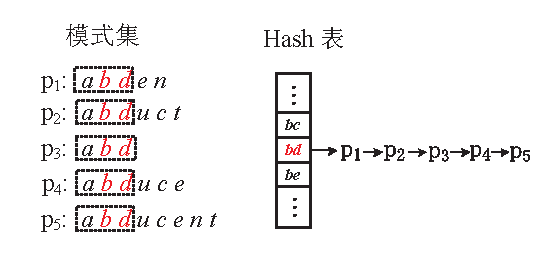
\includegraphics[height=4cm ,width=10cm]{figures/5_WM/WM_hash_table1.eps}
  \caption{WM算法为模式集构建的Hash表。}
  \label{fig:WM_hash_table1}
\end{figure}

这将导致在匹配过程中只要遇到字符块$bd$都需要遍历所有模式串,严重影响了
算法性能。实验证实,当模式集规模增大时,该问题愈加明显。亦有学者对此进
行了研究,主要集中于如何选择模式串的特征串,例如,文献\cite{}提出了一种
基于文本信息的特征串选择策略,但该方法需要文本的先验知识,而这往往是未
知的;文献\cite{Tan2011} 给出了一种基于机器学习的特征串选择方法,但其实
现起来较为复杂,当模式集变化较快时,算法的预处理时间较长。下面给出一种
仅仅依赖于模式集自身信息,且易于实现的特征串选择方法:

首先,对所有长为$B$的字符块 $block_i, i=1 \sim |\Sigma|^B$, 计算其在给
定模式集中的出现频率即: $freq(block_i)=|P'|$, $P' \subseteq
P$且对$\forall p \in P'$, $block_i$都是$p$的子串。 然后在每个模式串中选
择出现频率最少的字符块并以此确定其特征串,这样选择出的特征串能够有效地
刻画模式串自身的特性,具有较强的区分度,可以有效地克服原算法存在的问题。
例如,对于上述的模式集,我们事先统计出每个字符块在该模式集中的出现频率,
如表 \ref{tab:block_freq} 所示(未出现的字块频率均为0):


\begin{table}[!htbp]
\centering
\vspace{-8pt}
\caption{所有长为2的字符块在给定模式集中的出现频率}
\begin{tabular}{|c|c|c|c|c|c|c|c|c|c|c|} \hline
  ... & $ab$ & $bd$ & $du$ & $uc$ & $ce$ &  $en$ & $nt$ & $ct$ & $de$ & ... \\\hline
  ... & 5 & 5 & 3 & 3 & 2 & 2 & 1 & 1 & 1 & ... \\
  \hline
  \end{tabular}
  \label{tab:block_freq}
\end{table}


对于 $p_1=abden$,可供选择的特征串为:$abd$, $bde$, $den$,由于在$bd$,
$de$,
$en$中$de$的出现频率最低,所以选择$bde$作为$p_1$的特征
串:$\overline{p_1}=bde$。类似地,我们
有:$\overline{p_2}=uct$,$\overline{p_3}=abd$,$\overline{p_4}=uce$,
$\overline{p_5}=ent$。用这样的特征串构造出的Hash表如
图\ref{fig:WM_hash_table2}所示:

\begin{figure}[!h]
  \centering
  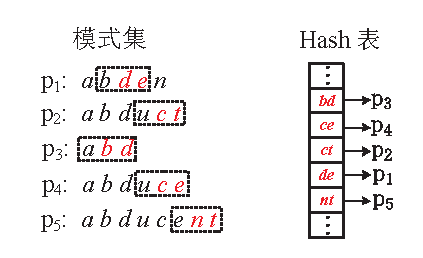
\includegraphics[height=4cm ,width=9cm]{figures/5_WM/WM_hash_table2.eps}
  \caption{DWM算法为模式集构建的Hash表。}
  \label{fig:WM_hash_table2}
\end{figure}

这种选择策略避免了由于模式串的聚集而造成哈希链过长的情况,并且在匹配时
遇到某个字符块将会搜索最有可能匹配该字块的模式串,减少了搜索范围,因为
我们在选择每个模式串的特征串时,都是选择其(相对)最具代表性的部分作为
特征串的。下面是具体算法:

\begin{algorithm}
  \caption{步骤 1: 计算字符块的出现频率}
  \label{alg:block_freq}
  \begin{algorithmic}[1]
    \REQUIRE ~~\\
    模式集 $P$。 \\
    \ENSURE ~~\\
    每个长为$B$的字符块在 $P$中模式的出现频率。\\
    \STATE
    \STATE 创建长为$|\Sigma|^B$的数组$freq$(并将其元素初始化为0),用来记录字符块
    的出现频率。
    \STATE 创建长为$|\Sigma|^B$的数组$tag$,用来标记模式串中的字符块是
    否已经出现过。
    \STATE 变量$j$用于标记模式中字符块的起始位置。
    \STATE $block_{ij}$表示模式串$p_i$中,起始于位置$j$的字符块。
    \FOR{ $\forall p_i \in P$}
    \STATE 将$tag$数组清零。
    \FOR{$p_i$中每一个长为$B$的字符块 $block_{ij}$, $j=1 \sim |p_i|-B+1$}
    \IF{$tab[block_{ij}]\neq0$}
    \STATE $freq[block_{ij}]$ \leftarrow $freq[block_{ij}]+1$
    \STATE $tab[block_{ij}]=1$
    \ENDIF
    \ENDFOR
    \ENDFOR
    \STATE
    \RETURN $freq$ 数组。
  \end{algorithmic}
\end{algorithm}


注意,如果一个字符块在某个模式串中出现多次,只按出现一次算,因此在扫描
每个模式串时,需要一个标记表$tag$,来记录某个字符块是否在该模式串中出现
过。对于模式串$p_i$,其包含的长为$B$的字符块数为$|p_i|-B+1$,而对每个模
式串,算法将扫描其中所有长为$B$的字符块,若模式集包含$k$个模式串,则总
的扫描次数将为:$\sum_{i=1}^{k}(|p_i|-B+1)$,因此,步骤 1的时间复杂度
为:$O(模式串长之和)$.

\begin{algorithm}
  \caption{步骤 2: 选择特征串}
  \label{alg:choose_signature}
  \begin{algorithmic}[1]
    \REQUIRE ~~\\
    模式集 $P$, 字符块频率表 $ferq$。 \\
    \ENSURE ~~\\
    每个模式串的特征串。\\
    \STATE
    \STATE $lsp \leftarrow$ 最短模式串长。
    \STATE 变量 $min\_block$ 代表当前模式串中出现频率最少的字符块。
    \STATE 
    \FOR{ $\forall p_i \in P$}
    \STATE $j \leftarrow lsp-B+1$
    \STATE $min\_block \leftarrow block_{ij}$
    \FOR{$p_i$中每个长为$B$的字符块: $block_{ij}$, $j=lsp-B+2 \sim |p_i|-B+1$}
    \IF{$freq[block_{ij}] < freq[min\_block]$}
    \STATE $min\_block \leftarrow block_{ij}$
    \STATE 选择以min\_block结尾,长为m的字符串作为的特征串。
    \ENDIF
    \ENDFOR
    \ENDFOR
  \end{algorithmic}
\end{algorithm}

对于任意模式串 $p_i$,其可供选择的特征串共有$|p_i|-lsp+1$个。对每个模
式串$p_i$,必须从起始位置为$lsp-B+1 \sim |p_i|-B+1$的这些字符块中,选
择频率最小的一个作为特征串的后缀,而不是从头开始选取。若模式集包含$k$
个模式串,则步骤 2需要扫描的字符块总数为$\sum_{i=1}^{k}(|p_i|-lsp+1)$,
因此其时间复杂度也为:O(模式串长之和)。综合以上两步,DWM预处理过程的时
间复杂度仅为:O(模式串长之和)。极低的时间复杂度和简单的实现过程保证了
DWM的可行性,其增加的额外的预处理开销微乎其微,因此完全适用于不断变化
的模式集。注意:DWM增加Hash表中哈希链的数目,导致了Shift表中值为0的项
增加,这会在一定程度上降低算法的跳转效率。但对于规模较小的模式集,性能
影响十分有限,且可以通过下一节将要介绍的哈希链加速技术来弥补;而当模式
集规模较大时,无论是原算法还是改进算法,Shfit表中几乎所有项都将为0,算
法跳转可能性大大降低,此时,算法的效率将主要取决于Hash表的表项分布,所
以对于较大规模的模式集,DWM明显地提升了原算法的性能,后面的实验证明了
该结论。

\subsection{加速哈希链的搜索(WM+)}
\label{sec:5_WM+}

原算法所构造的Prefix表效率很低,在匹配时,一旦遇到$Shift[block]=0$的情
形,要遍历整个$Hash[block]$所对应的链表来确定需要精确匹配的模式串,若链
表长度为$N$,其时间复杂度为$O(N)$,当哈希链很长且被频繁命中时,将会严重
影响算法性能。如果在构建哈希链时,事先按照特征串前缀哈希值的大小对模式
串进行排序,并为每条较长的链表建立相应的索引表,则在命中该哈希链时,只
需在索引表上进行二分查找,便可在$O(logn)$时间内找到需要进行精确匹配的模
式串,$n$为索引表的大小。索引表完全取代了原算法Prefix表的功能,且提高了
算法效率。

\begin{figure}[!h]
  \centering
  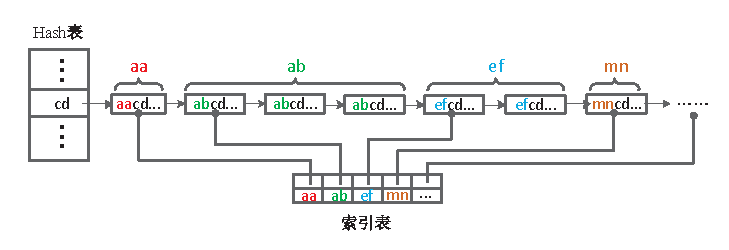
\includegraphics[height=5cm ,width=12cm]{figures/5_WM/WM_index.eps}
  \caption{为长哈希链建立索引表结构。}
  \label{fig:WM_index}
\end{figure}

图\ref{fig:WM_index}显示了Hash表中字符块$cd$的哈希链表及为其建立的索引
表,假设$B=2$,前缀也取2个字符,最短模式串长$m=4$,对每个模式串(按照原
算法)取前4个字符作为其特征串。该哈希链中的所有模式串,按照其前缀哈希值
由小到大进行排序,这样前缀相同的模式串会被连续地排列在一起,依次遍历该
哈希链,对于每一个不同的前缀为其在索引表中建立一项,并将其指向哈希链中
具有该前缀的第一个模式串,这样构建的索引表也是有序的,通过它可以实现对
哈希链的快速搜索。例如,假设当前文本串的匹配窗口的后缀为$cd$,前缀
为$ef$,则无需遍历整个哈希链来寻找前缀为$ef$的模式串,只需要在索引表上
进行二分查找,便可迅速确定前缀为$ef$的模式串在哈希链中的起始位置,对从
起始位置开始的模式串依次进行精确匹配,直到遇到前缀不为$ef$的模式串为止
(无须记录其终止位置)。下面是建立索引表的算法(假设每条链表已经排好
序):

\chapter{总结与展望}
\label{chap:Conclusion}

本章将对全文工作进行总结, 然后提出进一步的研究方向.

\section{全文总结}

本文针对序列(字符串)挖掘领域中的三个重要问题,即多模式(字符串)匹配问
题,后缀排序问题,以及序列的最长公共子序列问题,进行了较为探索和研究,
主要工作包括以下三个方面:

\begin{enumerate}
\item 多模式匹配。 现有的基于内存的多模式匹配算法为模式集所构造的数据结
  构鲁棒性较差,性能易受到模式集自身特性(尤其是最短模式串长)的影响,同
  时可伸缩性较差,在处理大规模模式集时,性能往往无法满足实际需求。针对
  此问题,本文设计并实现了一种高效的多模式匹配引擎。 该引擎包括过滤与核
  实两个模块:过滤模块基于位图结构,所有操作均基于底层位运算,因此能够
  快速地过滤掉文本串中不可能出现匹配的位置;对每一个潜在的匹配位置,调
  用核实模块来确认是否有模式串出现。 核实模块基于一种被称为“自适应匹配
  树”的树形结构,树中的每个节点都保存了模式集的一部分片段,节点内部的
  存储结构将根据自身所保存的模式集片段的特征(即片段长度和片段数量)进行
  自适应地调整,以达到时间效率和空间效率的最佳平衡。 由于每个节点的自适
  应性,使得对于任何特性的模式集,所构造的自适应匹配树都能够保持最高效
  的形态。因此,相比现有算法拥有更好的鲁棒性和可伸缩性。

  另外,对实际中广泛使用的多模式匹配算法---Wu-Manber(WM)算法进行了改进,
  提高了其在地处理较大规模模式集时的效率。不同于WM算法每次都选取模式串
  的前lsp(即最短模式串长)个字符作为其特征串,改进算法通过动态地选取每个
  模式串的特征串,使得模式串能够更加均匀地分布于哈希表中;同时,为哈希
  表的模式串链表设计了索引表,通过在索引表上进行二分查找,能够进一步提
  高算法的搜索速度。实验证实,这两项改进有效地提升了算法在处理较大规模
  模式集时的性能。

\item 后缀排序。基于传统的qsufsort算法框架,提出了一种改进型的后缀排序
  算法---dsufsort。 在传统qsufsort算法的每一轮中,所有后缀都将依据定长
  前缀(即在第$k$轮中,根据每个后缀长为$2^k$的后缀)被排序,这意味着
  前$2^k$个字符都相同的后缀,无法在第$k$轮中被确定顺序,这样,对于那些
  具有很长公共前缀的后缀,需要许多轮才能被确定顺序。为了解决该问
  题,dsufsort算法将记录并维护后缀数组中每个未排序桶的深度,在每一轮排
  序中,将根据待排序桶的深度对其中的后缀进行排序,
  这使得在第$k$轮中,后缀可以基于长度超过$2^k$的前缀被排序,从而那些
  前$2^k$个字符相同的后缀便可在第$k$轮中被确定顺序, 因此,dsufsort算法
  仅需要较少的轮数就可以完成排序。 此外,由于桶的深度具有累加性,因此,
  对于具有很长公共前缀的后缀,dsufsort算法可以更快速地完成排序。

\item 求序列的最长公共子序列。 现有算法在求解最长公共子序列问题时通常需
  要构建有向无环图,在图构造好之后通过搜索其中的最长路径来构建相应的最
  长公共子序列。然而,由于图中的节点数量过多,会导致大量的内存消耗,同
  时,在大规模图中搜索最长路径会花费较长的运行时间。 针对此问题,本文提
  出了一种新的层次化图模型---Leveled-DAG,及其相应的构建算法。 不同于现
  有的算法在构造有向无环图时,需要保存所有产生的节点,并在图构造好之后
  通过搜索其中的最长路径来构建相应的最长公共子序列, Leveled-DAG模型可
  以在建图的过程中实时地构建目标序列的最长公共子序列,并及时删除那些对
  构建最长公共子序列没有任何影响的无用节点。在任一时刻,Leveled-DAG只需
  保存最新产生的一层节点以及前面产生的入度不为0的节点,并且,随着构建过
  程的进行,图中的节点数将会逐渐减少,最终将仅剩余一个节点,所有目标序
  列的最长公共子序列都保存在该节点中。 得益于实时地构造最长公共子序列及
  删除无用节点,Leveled-DAG相比现有算法在时间和空间效率上都有较大提升。
  \end{enumerate}

\section{工作展望}

本文对序列挖掘中的三个关键问题:多模式匹配、后缀排序、以及最长公共子序
列问题,进行了较为深入的研究,分别提出了几种新的方法。然而,这些方法仍
有不成熟之处,在许多方面都值得进一步研究:

\begin{enumerate}
\item 对于自适应匹配树,研究更加高效的树节点的结构,可以从整体上提高核
  实过程的效率;同时,对自适应策略所依赖的各种参数,需要进行更加精细的
  设置。
\item 对于dsufsort算法,对桶的处理顺序会对算法的性能造成一定影响, 所以
  需要进一步研究最优的桶处理顺序。 其次, 用来记录桶深的数组可能会非常稀
  疏, 这会增加空间开销, 所以研究稀疏数组压缩技术也非常重要。
\item 对于Leveled-DAG 模型,如何更加高效地删除过时节点将极大的提高算法
  的性能;同时,由于算法需要大量的内存分配, 调整大小, 以及释放操作,因
  此需要寻找更高效的内存管理函数来取代由标准库提供的内存分配函数。

\end{enumerate}

 \XDUbackmatter{\bibliography{bib/phd}\nocite{*}}
 
\begin{thanks}

���������ڵ�ʦ��Ϥ��ָ������ɵģ������ĵ�ѡ�⵽���ĵ�׫д���޲���͸�ŵ�ʦ����Ѫ������ֵ���������֮�ʣ����Ե�ʦ�����������Լ�׻׻�̻��ʾ�����ĵĸ�л!

\end{thanks}

 
\begin{resume}

\section*{1.\hspace{0.75em}基本情况}
彭展,男,陕西西安人,~1986~年~3~月出生,西安电子科技大学~计算
机~学院~计算机应用技术~专业~2011~级博士研究生。
\section*{2.\hspace{0.75em}教育背景}
\begin{resumelist*}
  \resumelistitem 2004.08~~2008.06,西安电子科技大学,本科,专业:软件
  工程
  \resumelistitem 2008.08~~2011.03,西安电子科技大学,硕士研
  究生,专业:计算机软件与理论
  \resumelistitem 2011.03~\hspace{3.5em}, 西安电子科技大学,博士研
  究生,专业:计算机应用技术
\end{resumelist*}

\section*{3.\hspace{0.75em}攻读博士学位期间的研究成果}
\begin{resumelist}{\hspace{-0.25em}3.1\hspace{0.5em} 发表学术论文}

  \resumelistitem Zhan Peng, Yuping Wang. A Novel Efficient Graph
  Model for the Multiple Longest Common Subsequences (MLCS) Problem
  [J]. Frontiers in Genetics, 8:104, 2017. (SCI: , EI: ) (已录用)

  \resumelistitem Zhan Peng, Yuping Wang, and Wei Yue. A Fast Engine
  for Multi-String Pattern Matching[J]. International Journal of Pattern
  Recognition and Artificial Intelligence, 2017: 1750039. (SCI:, EI: )

  \resumelistitem Zhan Peng, Yuping Wang, Xingsi Xue and Jingxuan
  Wei. An Efficient Algorithm for Suffix Sorting[J]. International
  Journal of Pattern Recognition and Artificial Intelligence, 2016,
  30(6): 1659018. (SCI:, EI: )

  \resumelistitem Zhan, Peng, Wang Yuping, and Xue Jinfeng. An
  Improved Multi-pattern Matching Algorithm for Large-Scale Pattern
  Sets[C]. 2014 Tenth International Conference on Computational
  Intelligence and Security (CIS), IEEE, pp:197-200, 2014.

  \resumelistiem 
\end{resumelist}

\begin{resumelist}{\hspace{-0.25em}3.3\hspace{0.5em} 参与科研项目及获奖}
\resumelistitem XXX项目, 项目名称, 起止时间, 完成情况, 作者贡献。
\resumelistitem XXX, XXX, XXX等. 科研项目名称. 陕西省科技进步三等奖, 获奖日期.
\resumelistitem \ldots
\end{resumelist}
\end{resume}

\end{document}

%%% Local Variables:
%%% mode: latex
%%% TeX-master: t
%%% End:
